% !TeX spellcheck = en_GB
\begin{wrapfigure}{r}{8.7cm}
	\vspace{-0.75cm}
	\begin{subfigure}{4.3cm}
		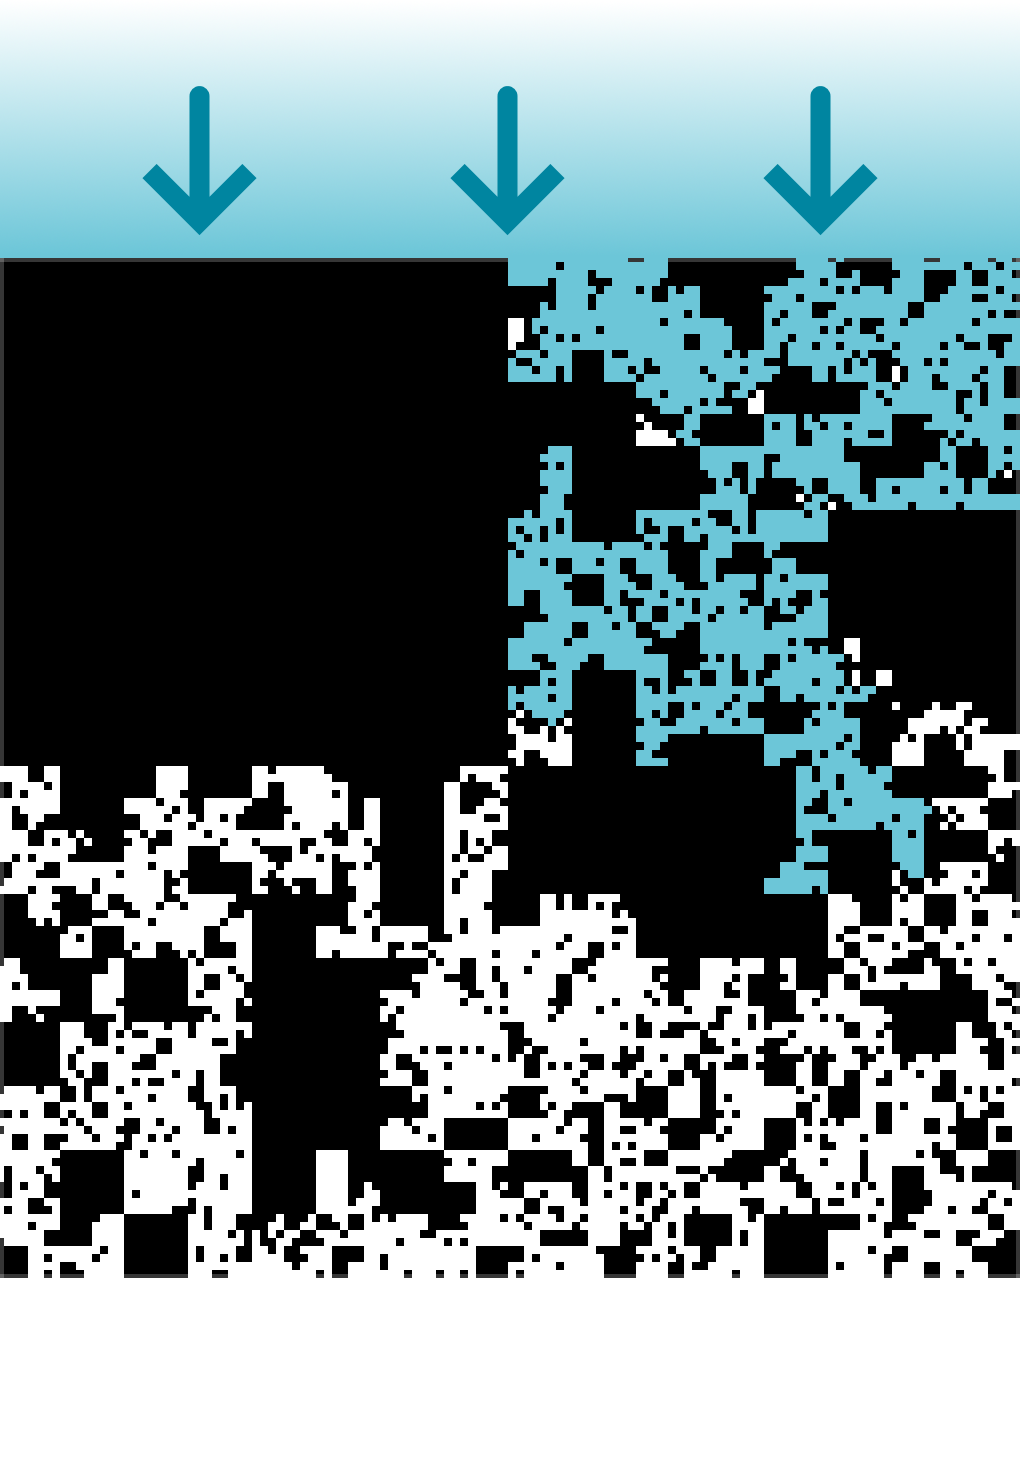
\includegraphics[width=4.2cm]{percolation_fluid}
		\centering
		\captionsetup{justification=centering}
		\caption{No vertical crossing: \\Fluid is stuck}
		\label{fig:percolationFluidNoCrossing}
	\end{subfigure}
	%\hspace{0.5cm}
	\begin{subfigure}{4.2cm}
		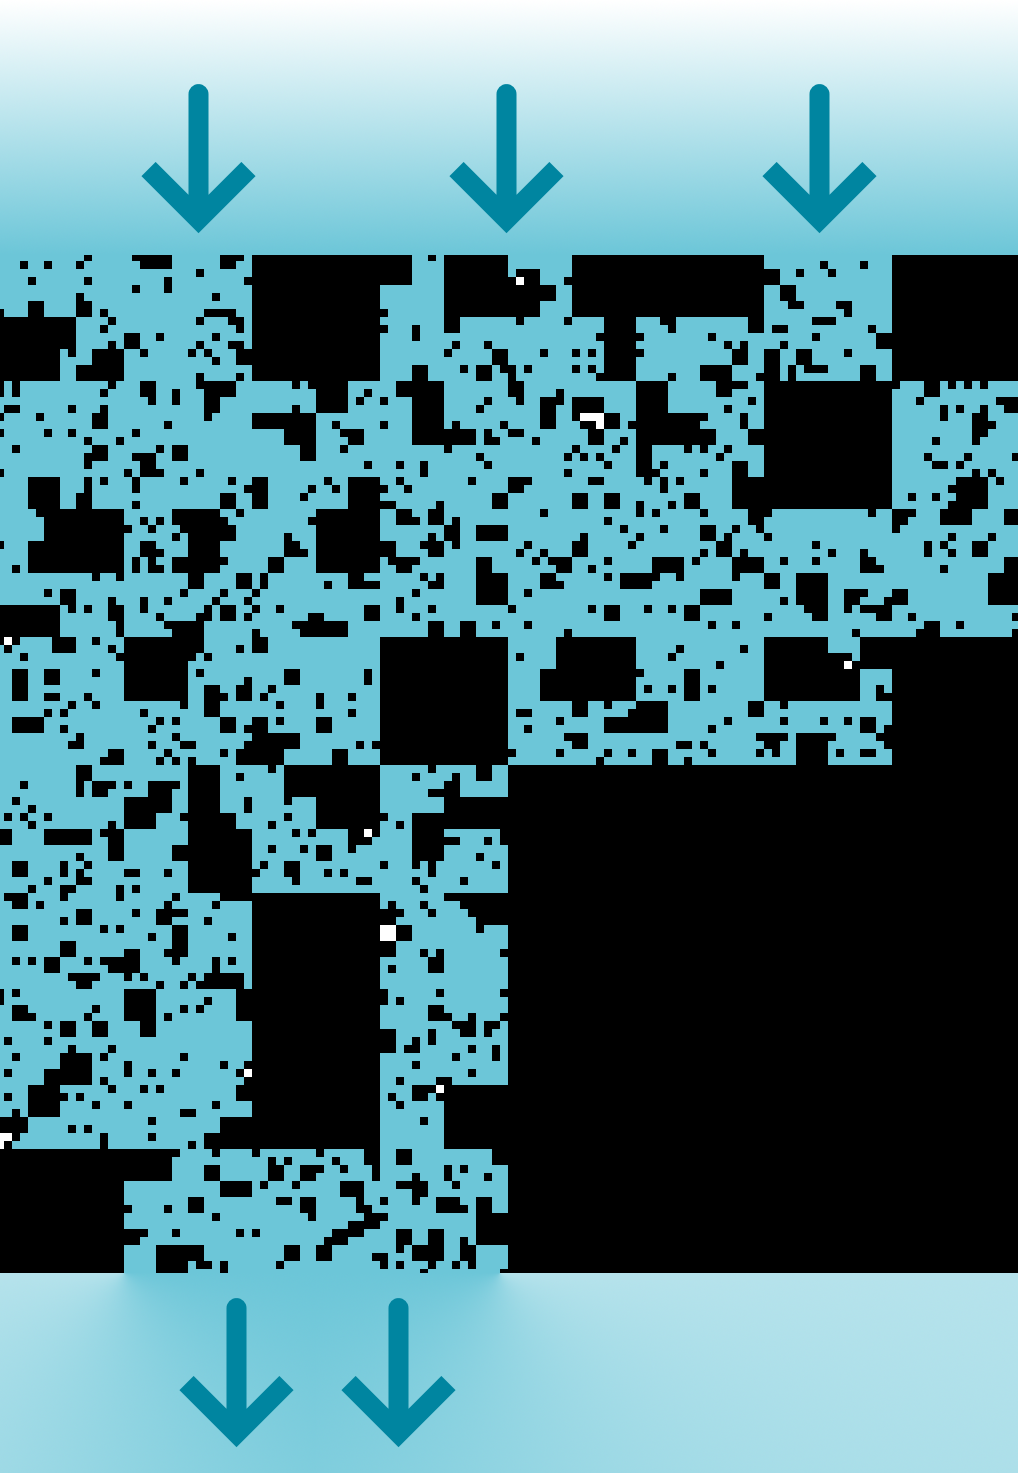
\includegraphics[width=4.2cm]{percolation_fluid_bis}
		\centering
		\captionsetup{justification=centering}
		\caption{Vertical crossings: \\Fluid can traverse}
		\label{fig:percolationFluidCrossing}
	\end{subfigure}
	\centering
	\caption{Percolations and Fluids}
	\label{fig:percolationFluid}
\end{wrapfigure}
\section{Percolation Crossings}
We are now interested in crossings from one side of the unit cuboid to the other side.
There is some physical motivation (introduced first in \cite{broadbent_hammersley_1957}) for such questions:
Suppose the percolation was a mathematical model for a physical material.
If $P$ has a crossing, then a fluid can pass through the material layer.
However, it will be stuck if there is no crossing.
The length of the crossing will tell how long it takes for the fluid to traverse the material.

The convention in mathematics is to study horizontal crossings, despite the clearer physical interpretation of vertical ones.
Rotating 90$^{\circ}$ transforms vertical crossings to horizontal ones and vice-versa, so studying either is equivalent.
We choose to stick to the mathematical convention.

\subsection{Types of Crossings}
There will be three types of crossing considered, according how the path is allowed to behave.

Consider a percolation $P$ on the unit cuboid $\left[ 0,1 \right]^D$ in $D$ dimensions, and let $\gamma: \left[ 0,1 \right] \to \left[ 0,1 \right]^D$ be a crossing of the cuboid, i.e. $\gamma(0) \in \{ 0 \} \times \left[ 0,1 \right]^{D-1}$ and $\gamma(1) \in \{ 1 \} \times \left[ 0,1 \right]^{D-1}$.
In the case of a finite percolation\footnote{i.e. $P \sim \text{Perc}^D(n,p,d)$ with $n,d < \infty$}, we can view a crossing as a walk on the cuboids of side $\nicefrac{1}{n^d}$.

\paragraph{Straight}
The crossing is said to be straight if $\gamma(y) = y \times (x_2,\dots,x_D)$.
That is, if the path goes on a direct line from one side to the other.
Only one step direction is allowed.
%Refer to fig. \ref{fig:crossing-straight}.

\paragraph{Semi-Straight}
The crossing is said to be semi-straight if $\forall \, 0 \leq y < z \leq 1, \ \gamma(y)_0 < \gamma(z)_0$\footnote{Writing $\gamma(y)_0$ for the first component of $\gamma(y)$.}.
That is, if the path never goes backwards.
This allows steps in $2D-1$ direction: all the possible directions except $(-1,0,\dots,0)$.
%Refer to fig. \ref{fig:crossing-semi-straight}.

\paragraph{Non-Straight}
If the crossing is neither straight or semi-straight, then it is non-straight.
In the latter case, all steps directions are allowed.
%Refer to fig. \ref{fig:crossing-non-straight}.

The following (fig. \ref{fig:crossingTypes}) illustrate the different types of crossings in two dimensions (the easiest to picture), extension to greater dimensions is straightforward.
\begin{figure}[!h]
	\begin{subfigure}{0.3\linewidth}
		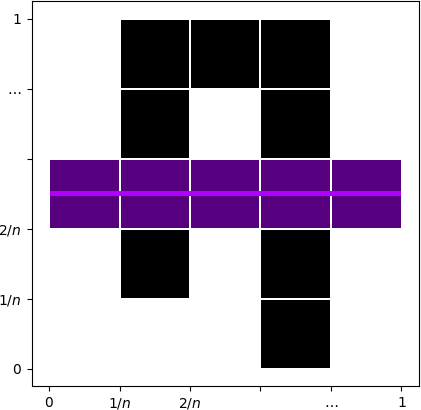
\includegraphics[width=5.4cm]{crossing-straight}
		\centering
		\captionsetup{justification=centering}
		\caption{Straight}
		\label{fig:crossingStraight}
	\end{subfigure}
	\hspace{0.04\linewidth}
	\begin{subfigure}{0.3\linewidth}
		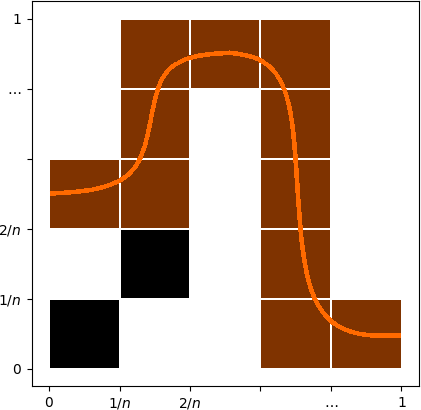
\includegraphics[width=5.4cm]{crossing-semi-straight}
		\centering
		\captionsetup{justification=centering}
		\caption{Semi-Straight}
		\label{fig:crossingSemiStraight}
	\end{subfigure}
	\hspace{0.04\linewidth}
	\begin{subfigure}{0.3\linewidth}
		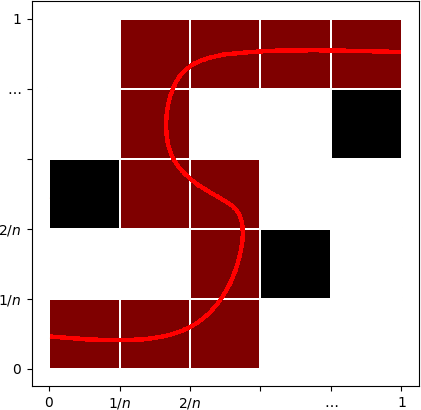
\includegraphics[width=5.4cm]{crossing-non-straight}
		\centering
		\captionsetup{justification=centering}
		\caption{Non-Straight}
		\label{fig:crossingNonStraight}
	\end{subfigure}
	\caption{Crossing types studied.}
	\label{fig:crossingTypes}
\end{figure}
When talking about a "crossing" in general, we will assume it may be either straight, semi-straight, or non-straight.


\subsection{Percolation Crossings}
First, we are interested in crossings lying on the percolation $P$.

\subsubsection{Crossings Probability}
For a percolation $P \sim \text{Perc}^D(n,p,d)$, we look at the probability that a crossing exists.

\paragraph{Straight Crossings}
This case is simple enough to derive an explicit formula for both classical and recursive percolations.
\subparagraph{Classical Percolation}
Take $P \sim \text{Perc}^D(\infty,p,1)$.
Then the probability that there is a straight crossing on the first line is $p^n$ (and is the same for the $n^{D-1}$ lines).
Thus, the probability that there is no crossing on any line is $1-(1-p^n)^{n^{D-1}}$, i.e. 
$$\mathbb{P}(P \text{ has a straight crossing}) = 1-(1-p^n)^{n^{D-1}} = \mathcal{O}(p^n f(n)) \text{ with } f(n) \text{ a polynomial of } n.$$
Thus, $\mathbb{P}(P \text{ has a straight crossing}) \to 0$, so it is almost sure that there is no crossing on a classical percolation $P$.

\subparagraph{Recursive Percolation}
Now take $P \sim \text{Perc}^D(n,p,\infty)$.

Let $Y^k$ be the number of straight crossings after $k$ filtrations, and $E^k = \mathbb{E}(Y^k)$ be the expected number of straight crossings\footnote{We count two crossings as different if they go through different cuboids.}.
Clearly, $E^0 = 1$, $E^1 = p^nn$, and recursively, $E^k = p^{n^k}nE^{k-1}$.
So in general, we get $E^k = n^k \prod_{i=1}^{k} p^{n^i}$, and $E^k \to 0$ as $k \to \infty$.
Now, $\mathbb{E}(Y^k) \to 0$ together with $Y^k \geq 0$ gives $\mathbb{P}(Y^k = 0) \to 1$.
So eventually, it is almost sure that a recursive percolation will have no straight crossings.

\paragraph{Numerics}
The study of semi-straight and non-straight crossings has to be done numerically.
All results can be found (in an interactive way) at \url{https://pauldubois98.github.io/PercolationFractalsStudy/crossings.html}.

\subparagraph{$D=2$}
As $d$ increases, it seems like the phase transition\footnote{We call phase transition the interval $\{ p \mid \mathbb{P}(\text{exists crossings}) \in (0,1) \}$.} shrinks.
One may conjecture that eventually, for a recursive percolation, the probability that there exists a crossing is either $0$ or $1$, and that there is a critical value $p_n$ that splits the two regimes.

For semi-straight crossings, transition occurs for a higher value of $p$\footnotemark.
However, the difference between non-straight and semi-straight crossing probabilities is very small.
For straight crossings, there is a significant difference.

As $n$ increases, we observe the same behaviour (transition phase shrinking), near $p=0.55$ for non-straight crossings and near $p=0.6$ for semi-straight crossings\addtocounter{footnote}{-1}\footnotemark.
\footnotetext{This makes sense as a semi-straight crossing is also a non-straight crossing.}

\begin{figure}[!h]
	\centering
	\begin{subfigure}{\textwidth}
		\begin{subfigure}{.49\textwidth}
			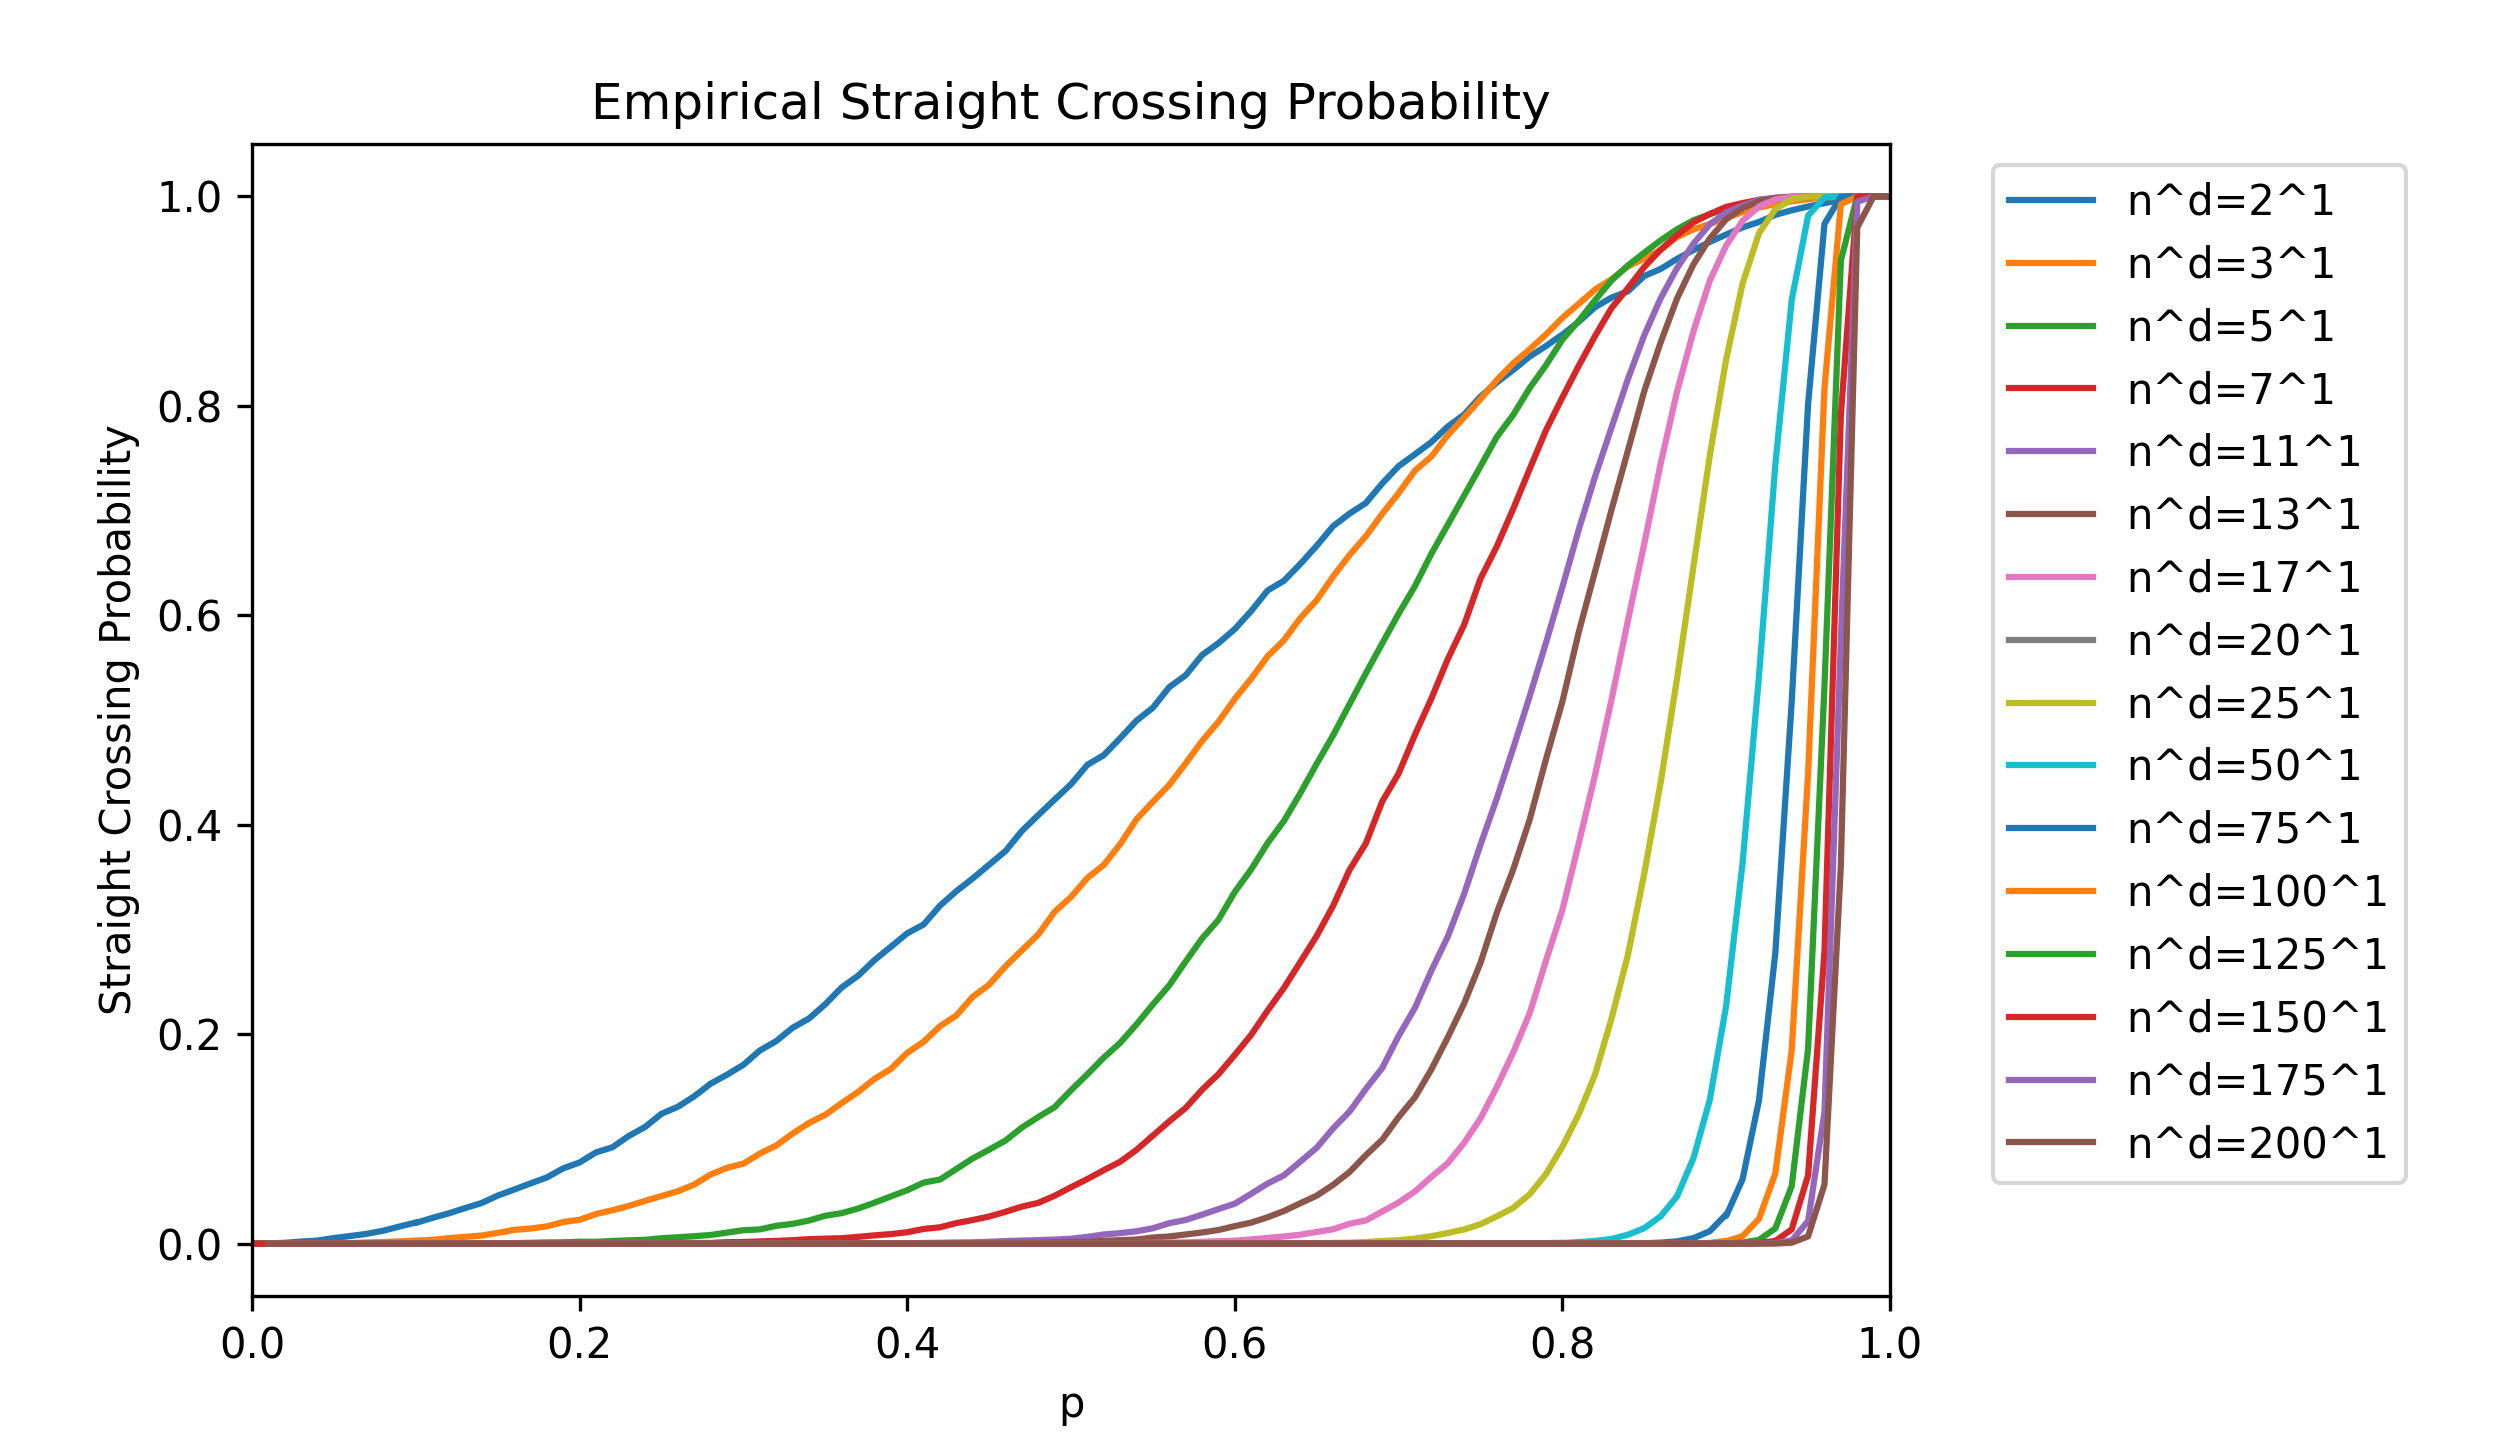
\includegraphics[width=8cm]{straight_crossing_proba_2D_ter}
			\centering
			\caption{Classical Percolation}
			\label{fig:crossingProbabilityClassical}
		\end{subfigure}
		\begin{subfigure}{.49\textwidth}
			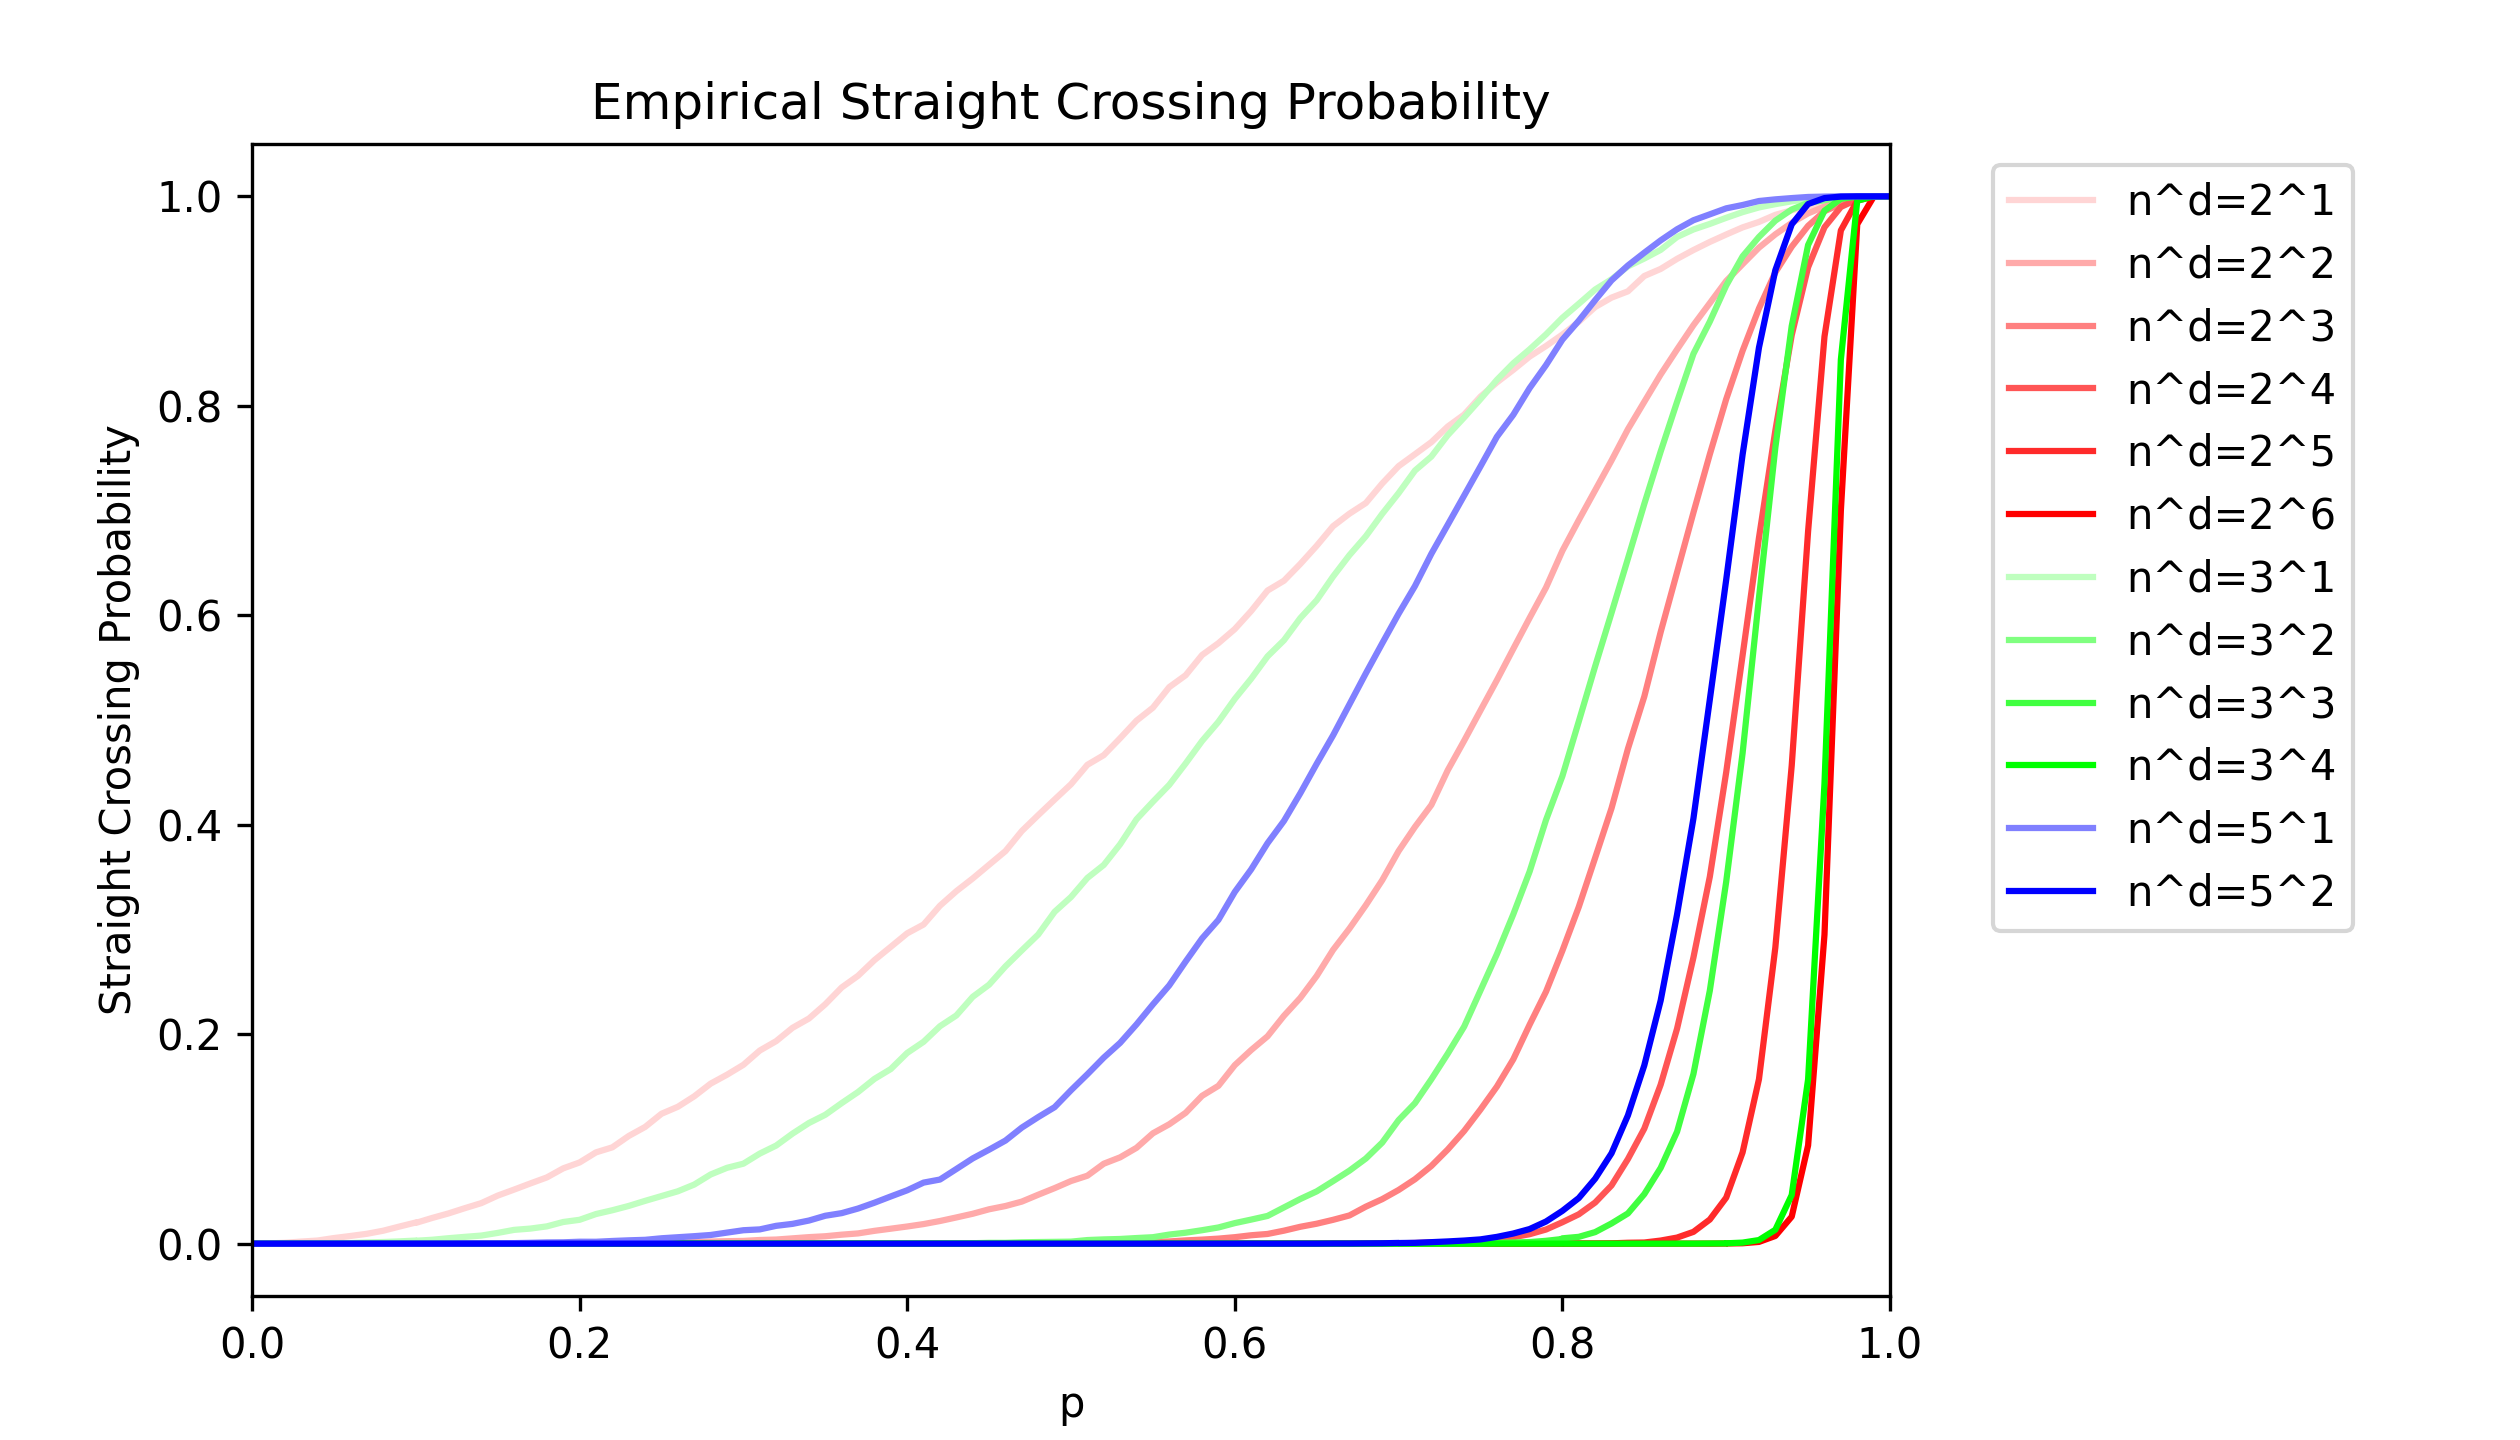
\includegraphics[width=8cm]{straight_crossing_proba_2D}
			\centering
			\caption{Recursive Percolation}
			\label{fig:crossingProbabilityRecursive}
		\end{subfigure}
	\end{subfigure}
	Straight
	
	\vspace{0.5cm}
	\begin{subfigure}{\textwidth}
		\begin{subfigure}{.49\textwidth}
			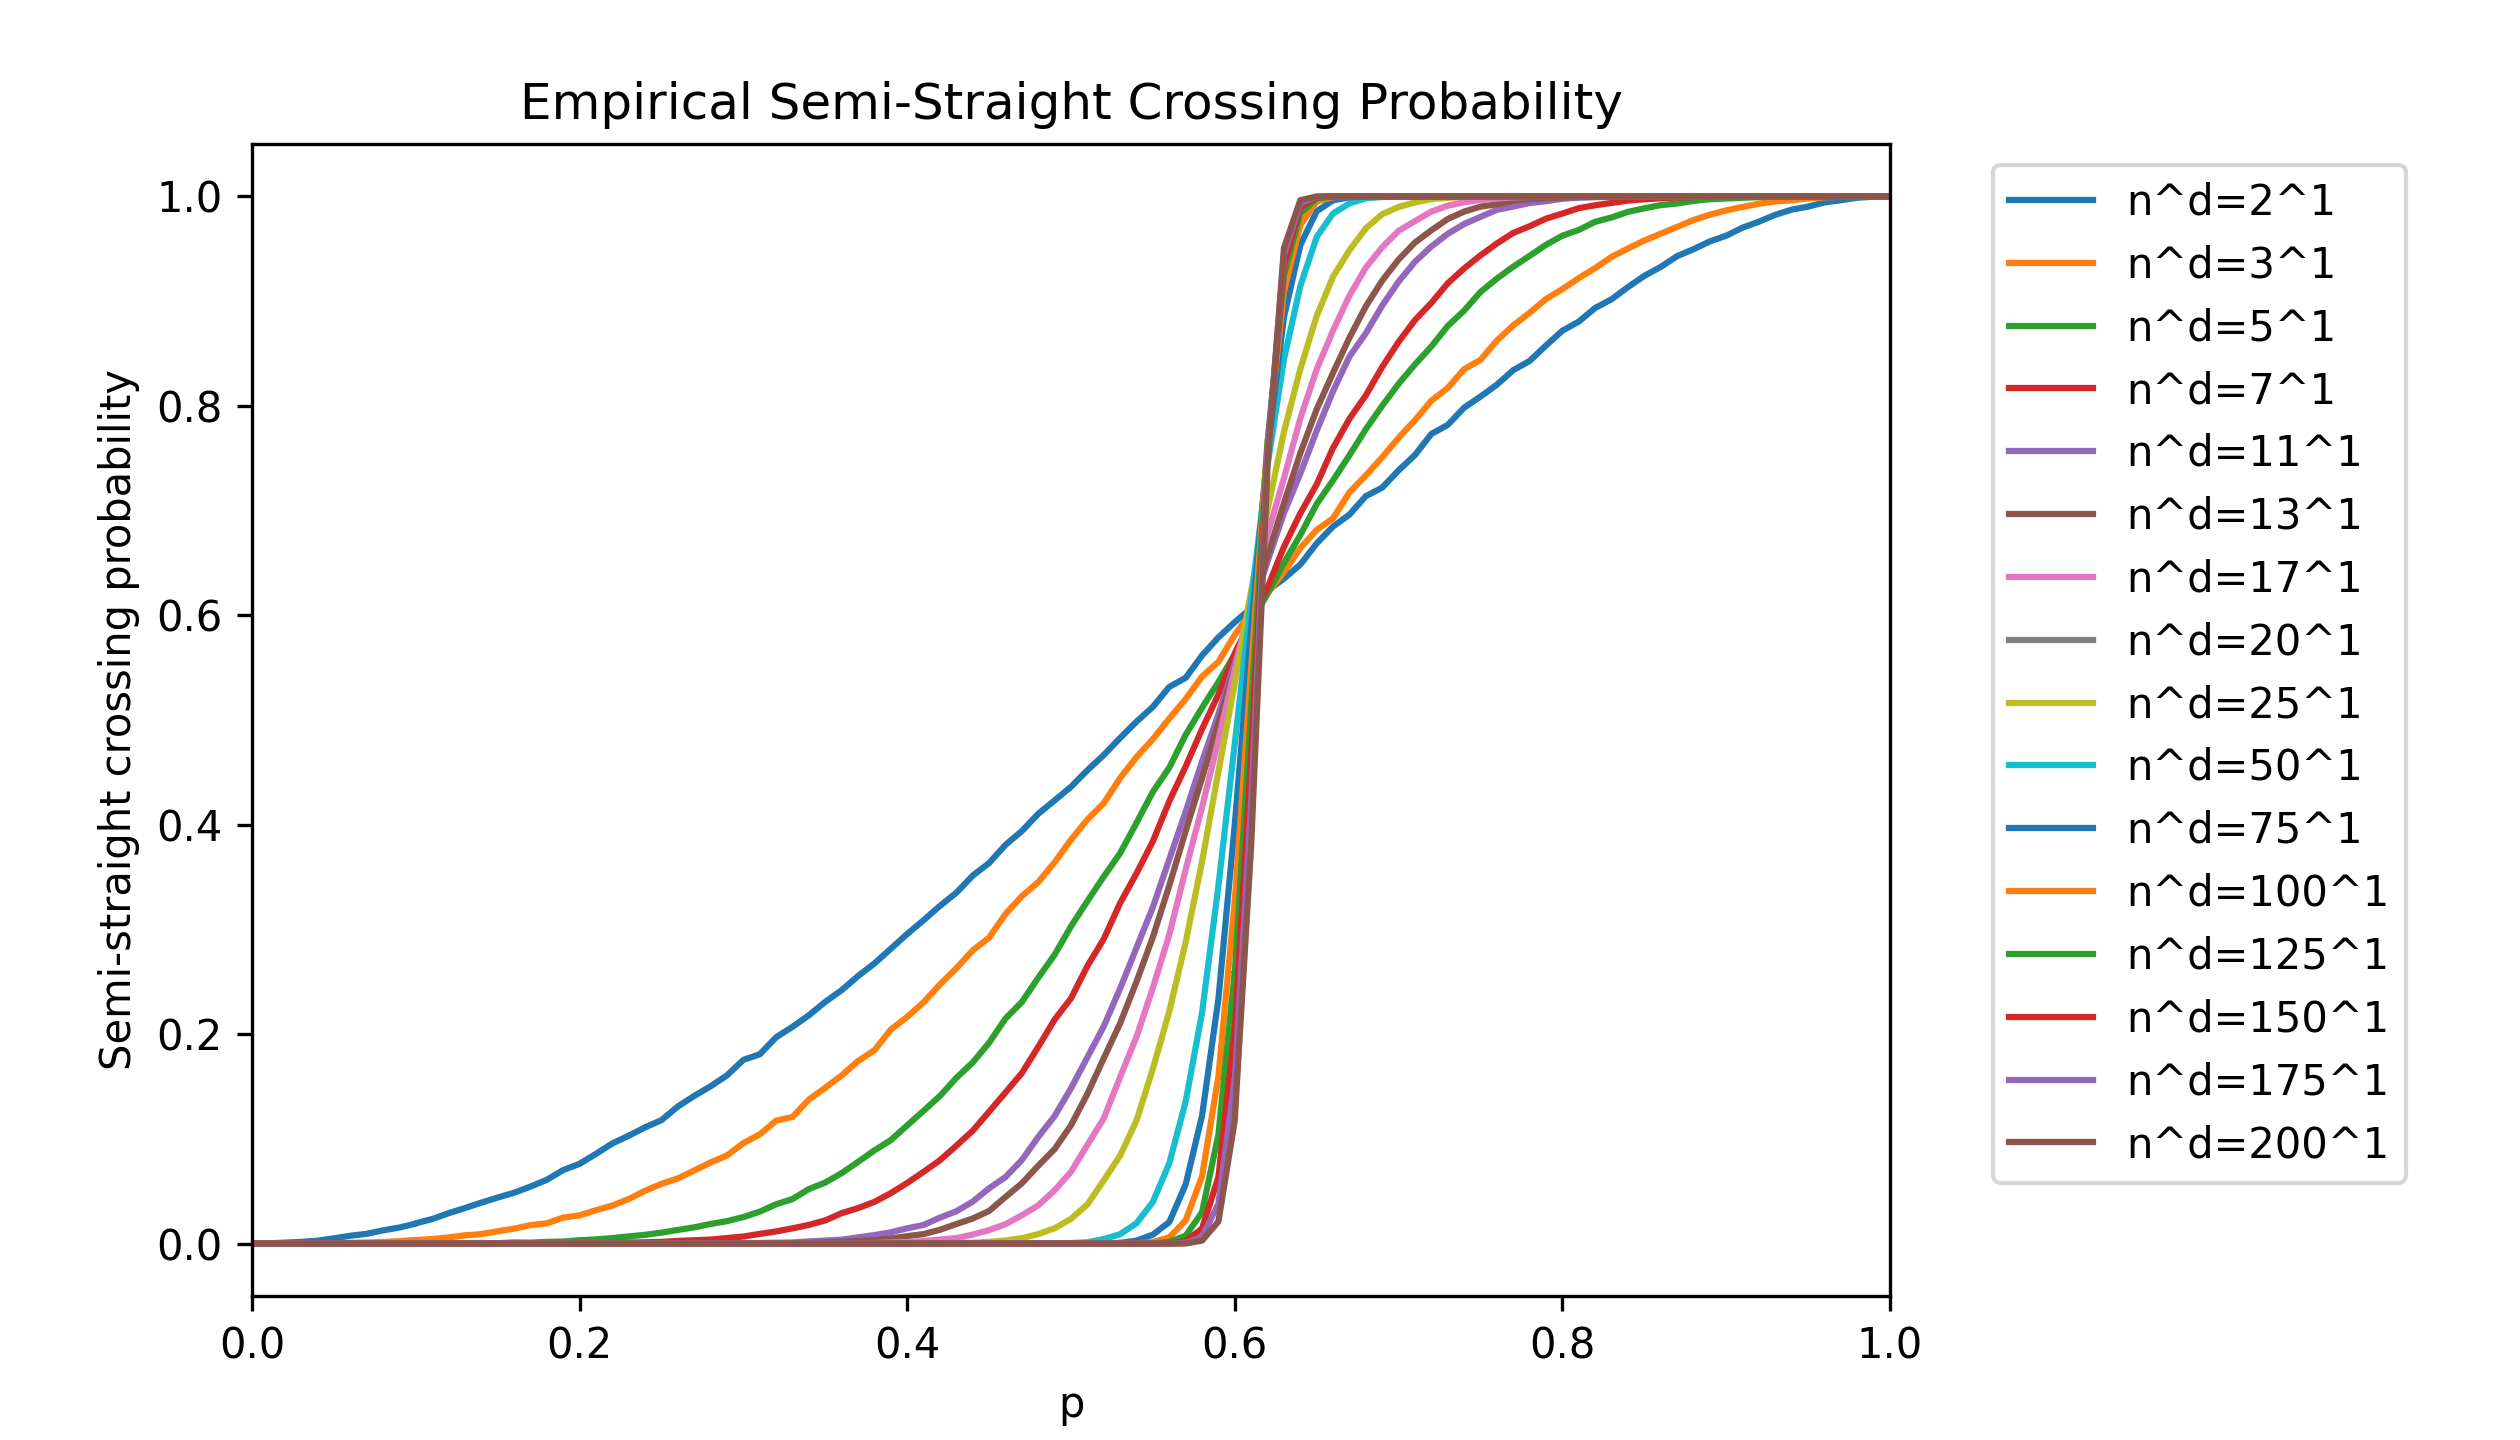
\includegraphics[width=8cm]{semi_straight_crossing_proba_2D_ter}
			\centering
			\caption{Classical Percolation}
		\end{subfigure}
		\begin{subfigure}{.49\textwidth}
			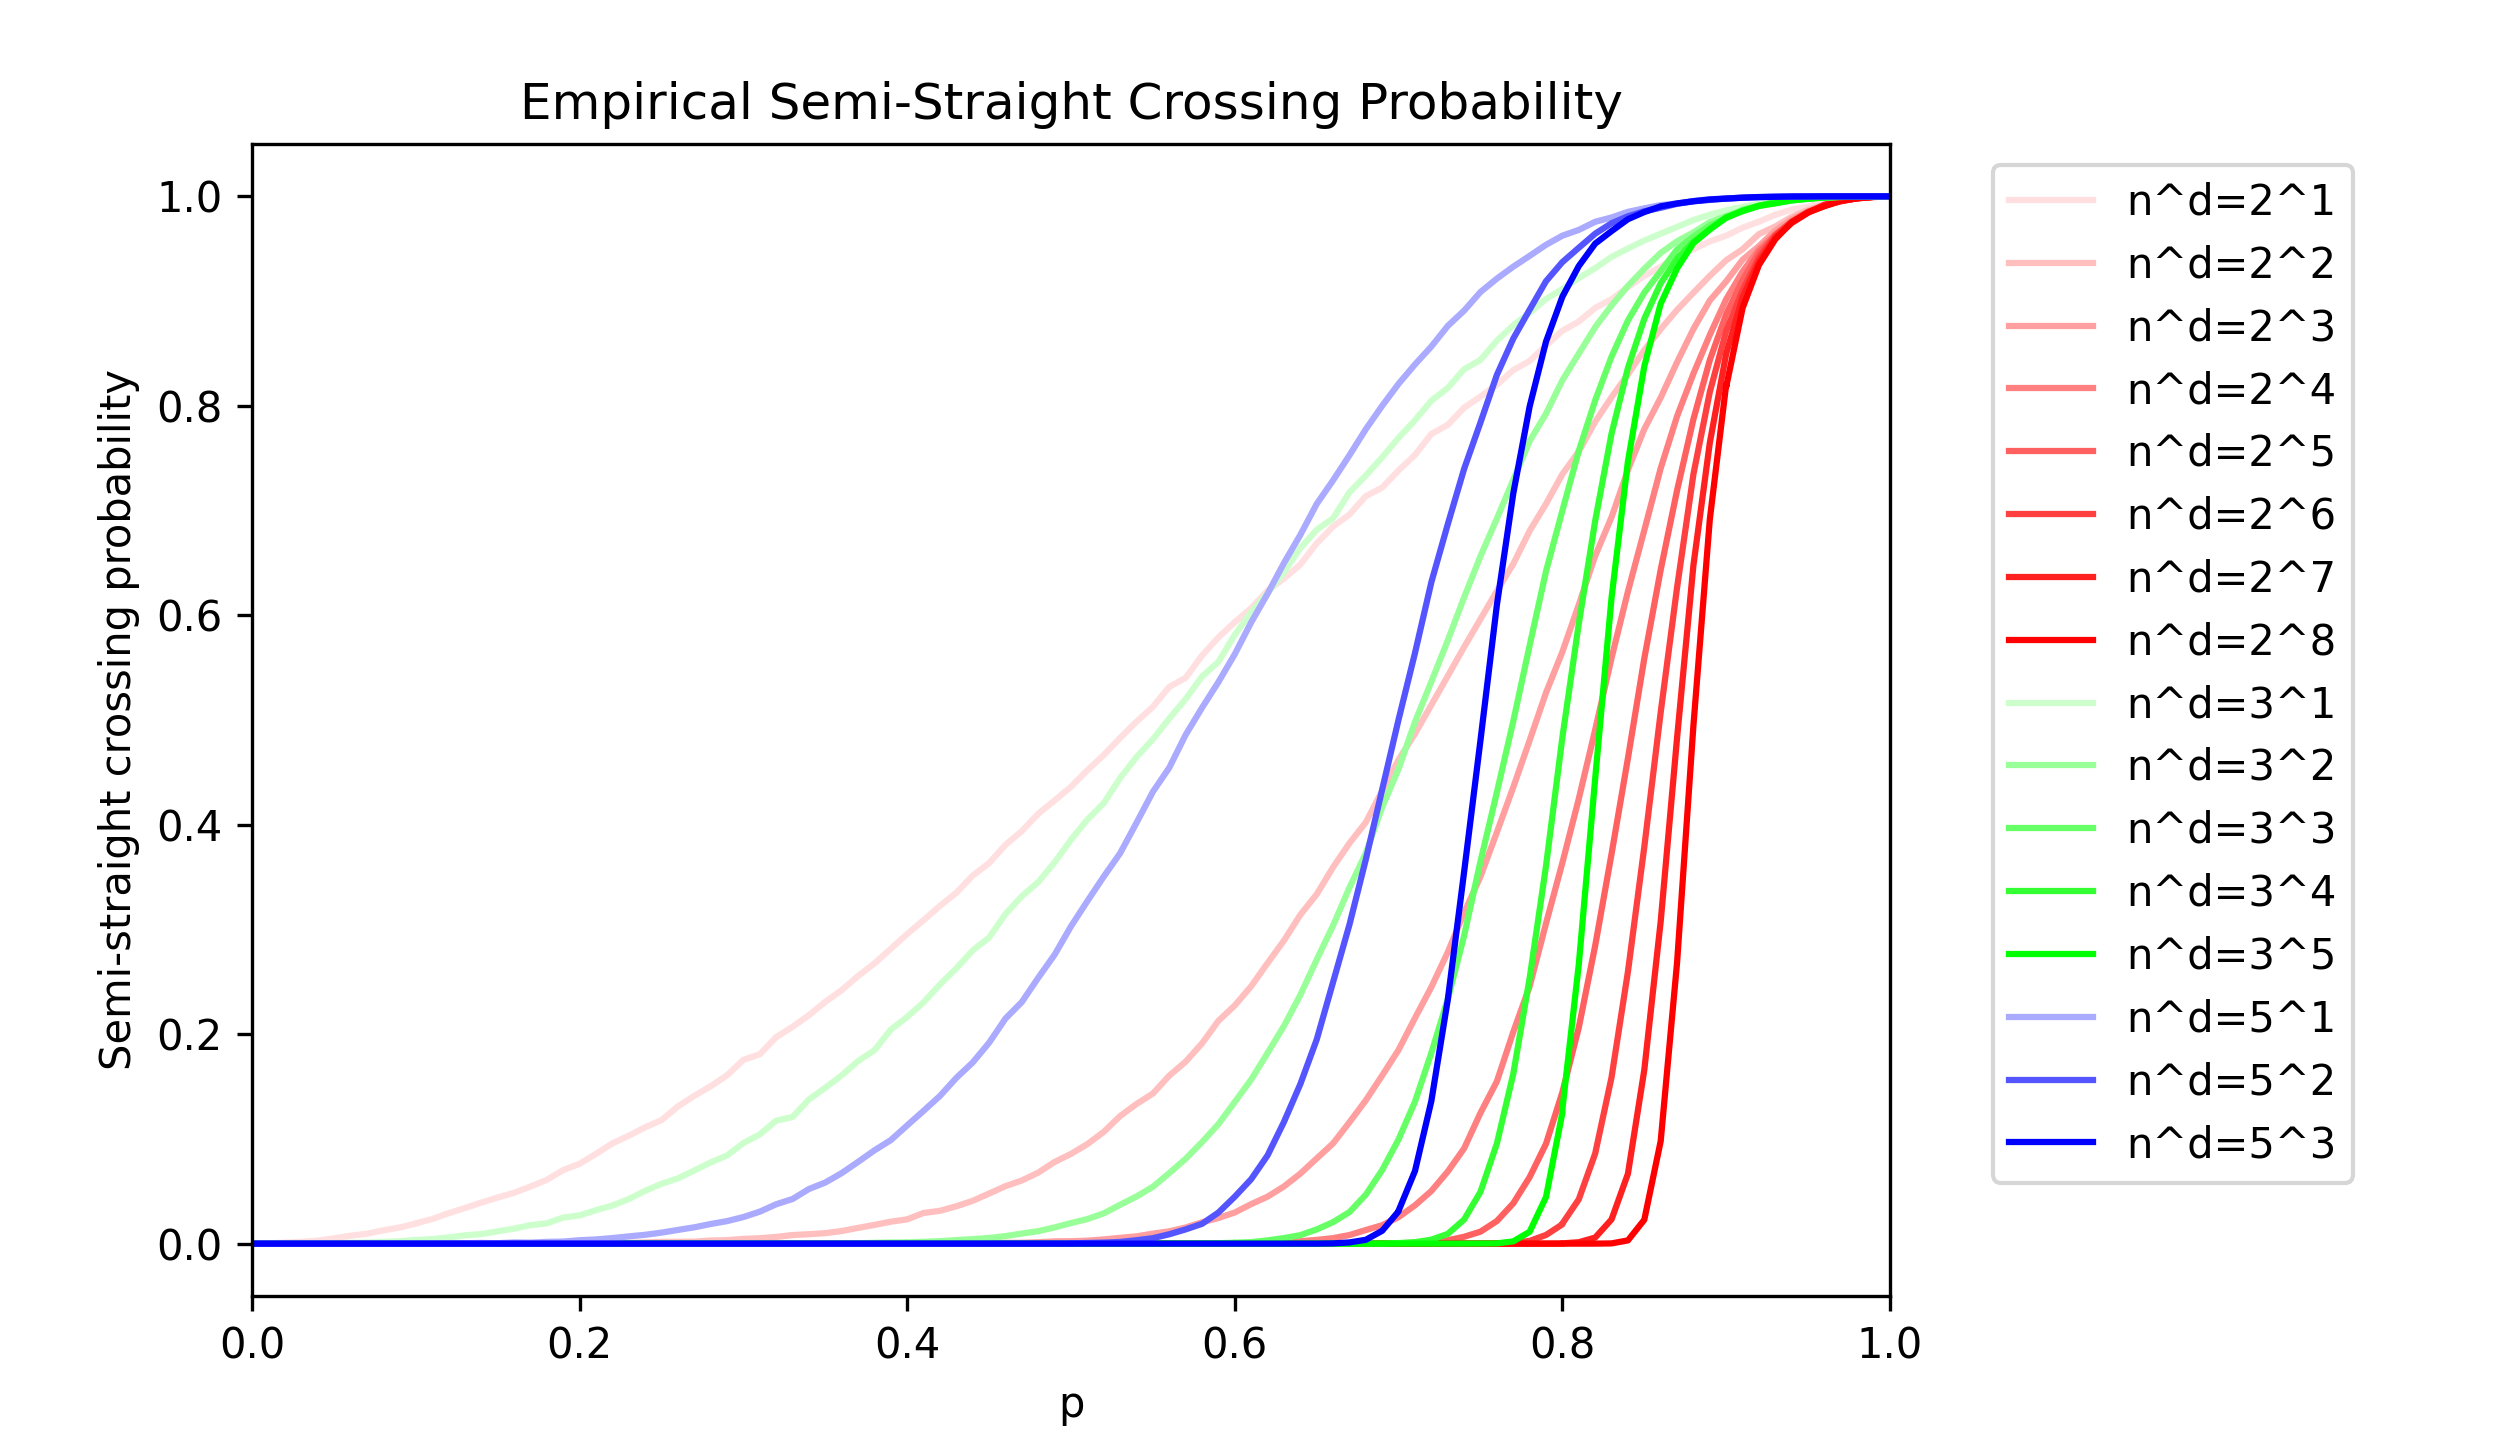
\includegraphics[width=8cm]{semi_straight_crossing_proba_2D}
			\centering
			\caption{Recursive Percolation}
		\end{subfigure}
	\end{subfigure}
	Semi-straight
	
	\vspace{0.5cm}
	\begin{subfigure}{\textwidth}
		\begin{subfigure}{.49\textwidth}
			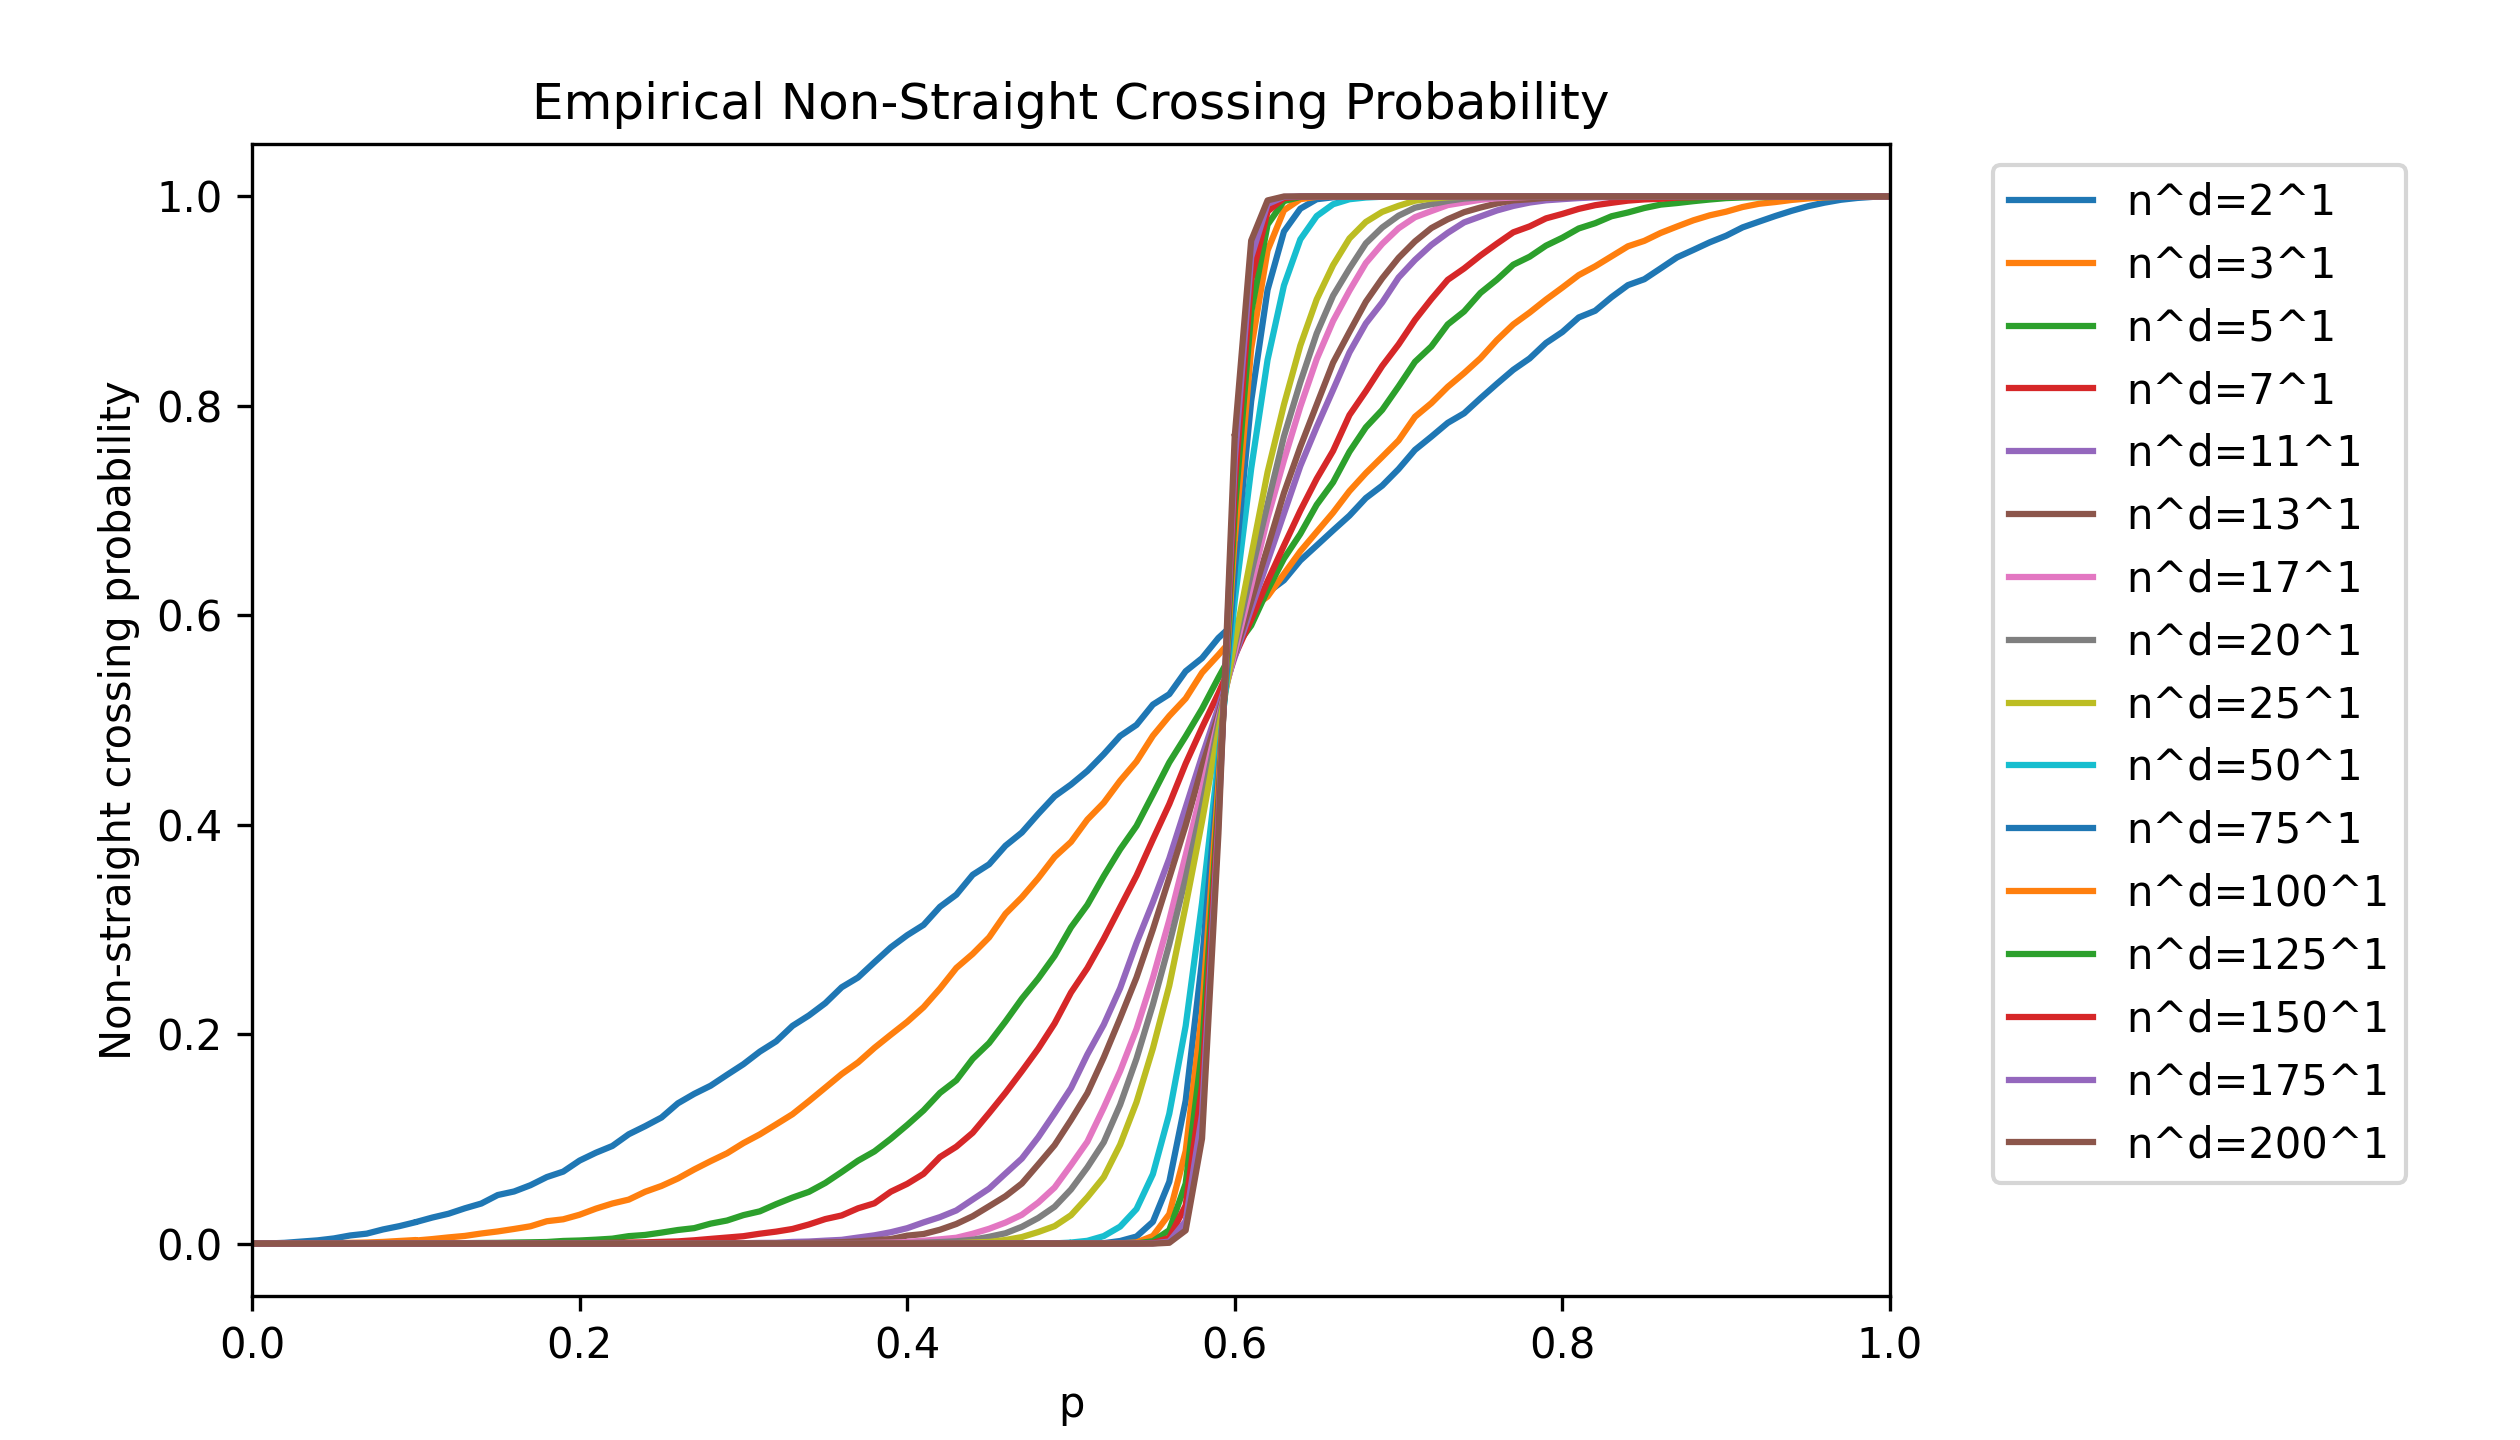
\includegraphics[width=8cm]{crossing_proba_2D_ter}
			\centering
			\caption{Classical Percolation}
		\end{subfigure}
		\begin{subfigure}{.49\textwidth}
			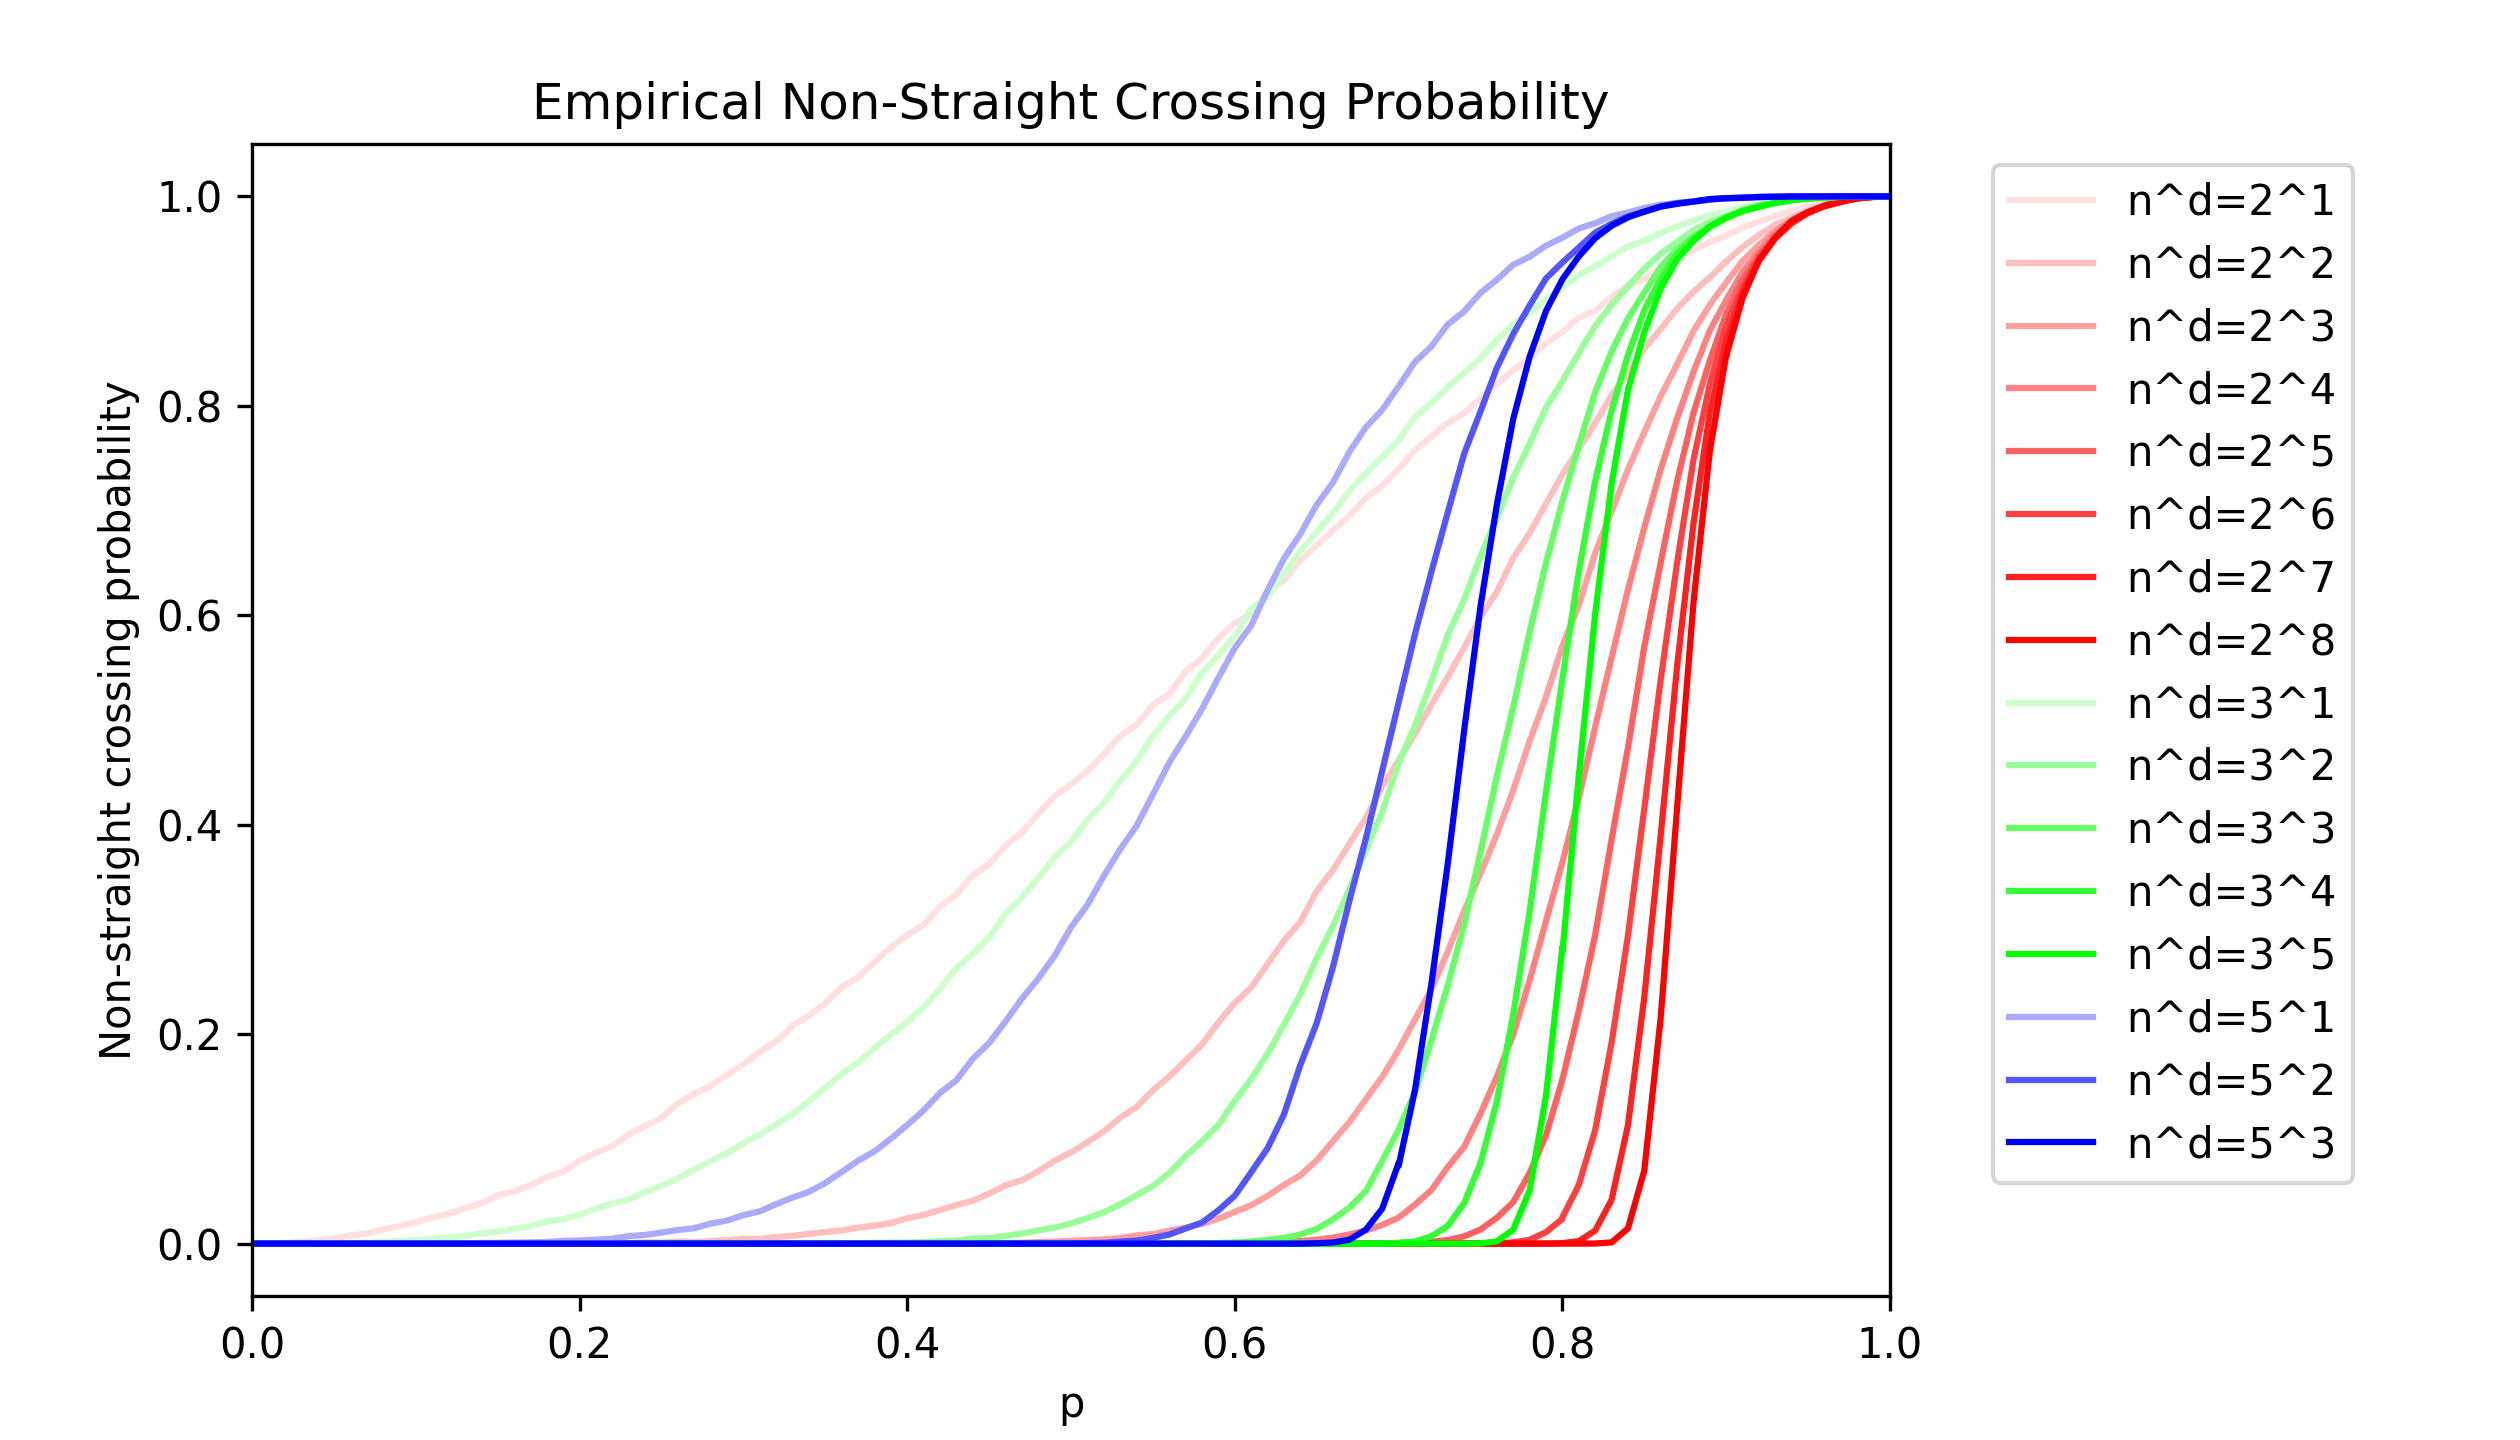
\includegraphics[width=8cm]{crossing_proba_2D}
			\centering
			\caption{Recursive Percolation}
		\end{subfigure}
	\end{subfigure}
	Non-straight
	
	\vspace{0.25cm}
	\caption{Crossing Probabilities, $D=2$}
	\label{fig:crossingProbabilities2D}
\end{figure}

\subparagraph{$D=3$}
In this case, we observe very similar behaviours, with transitions shifted to smaller values of $p$.
This makes sense as in 3D, there are more ways to go around a removed cuboid than in 2D (see fig. \ref{fig:crossingProbabilities3D}).

\begin{figure}[!h]
	\begin{subfigure}{0.45\linewidth}
		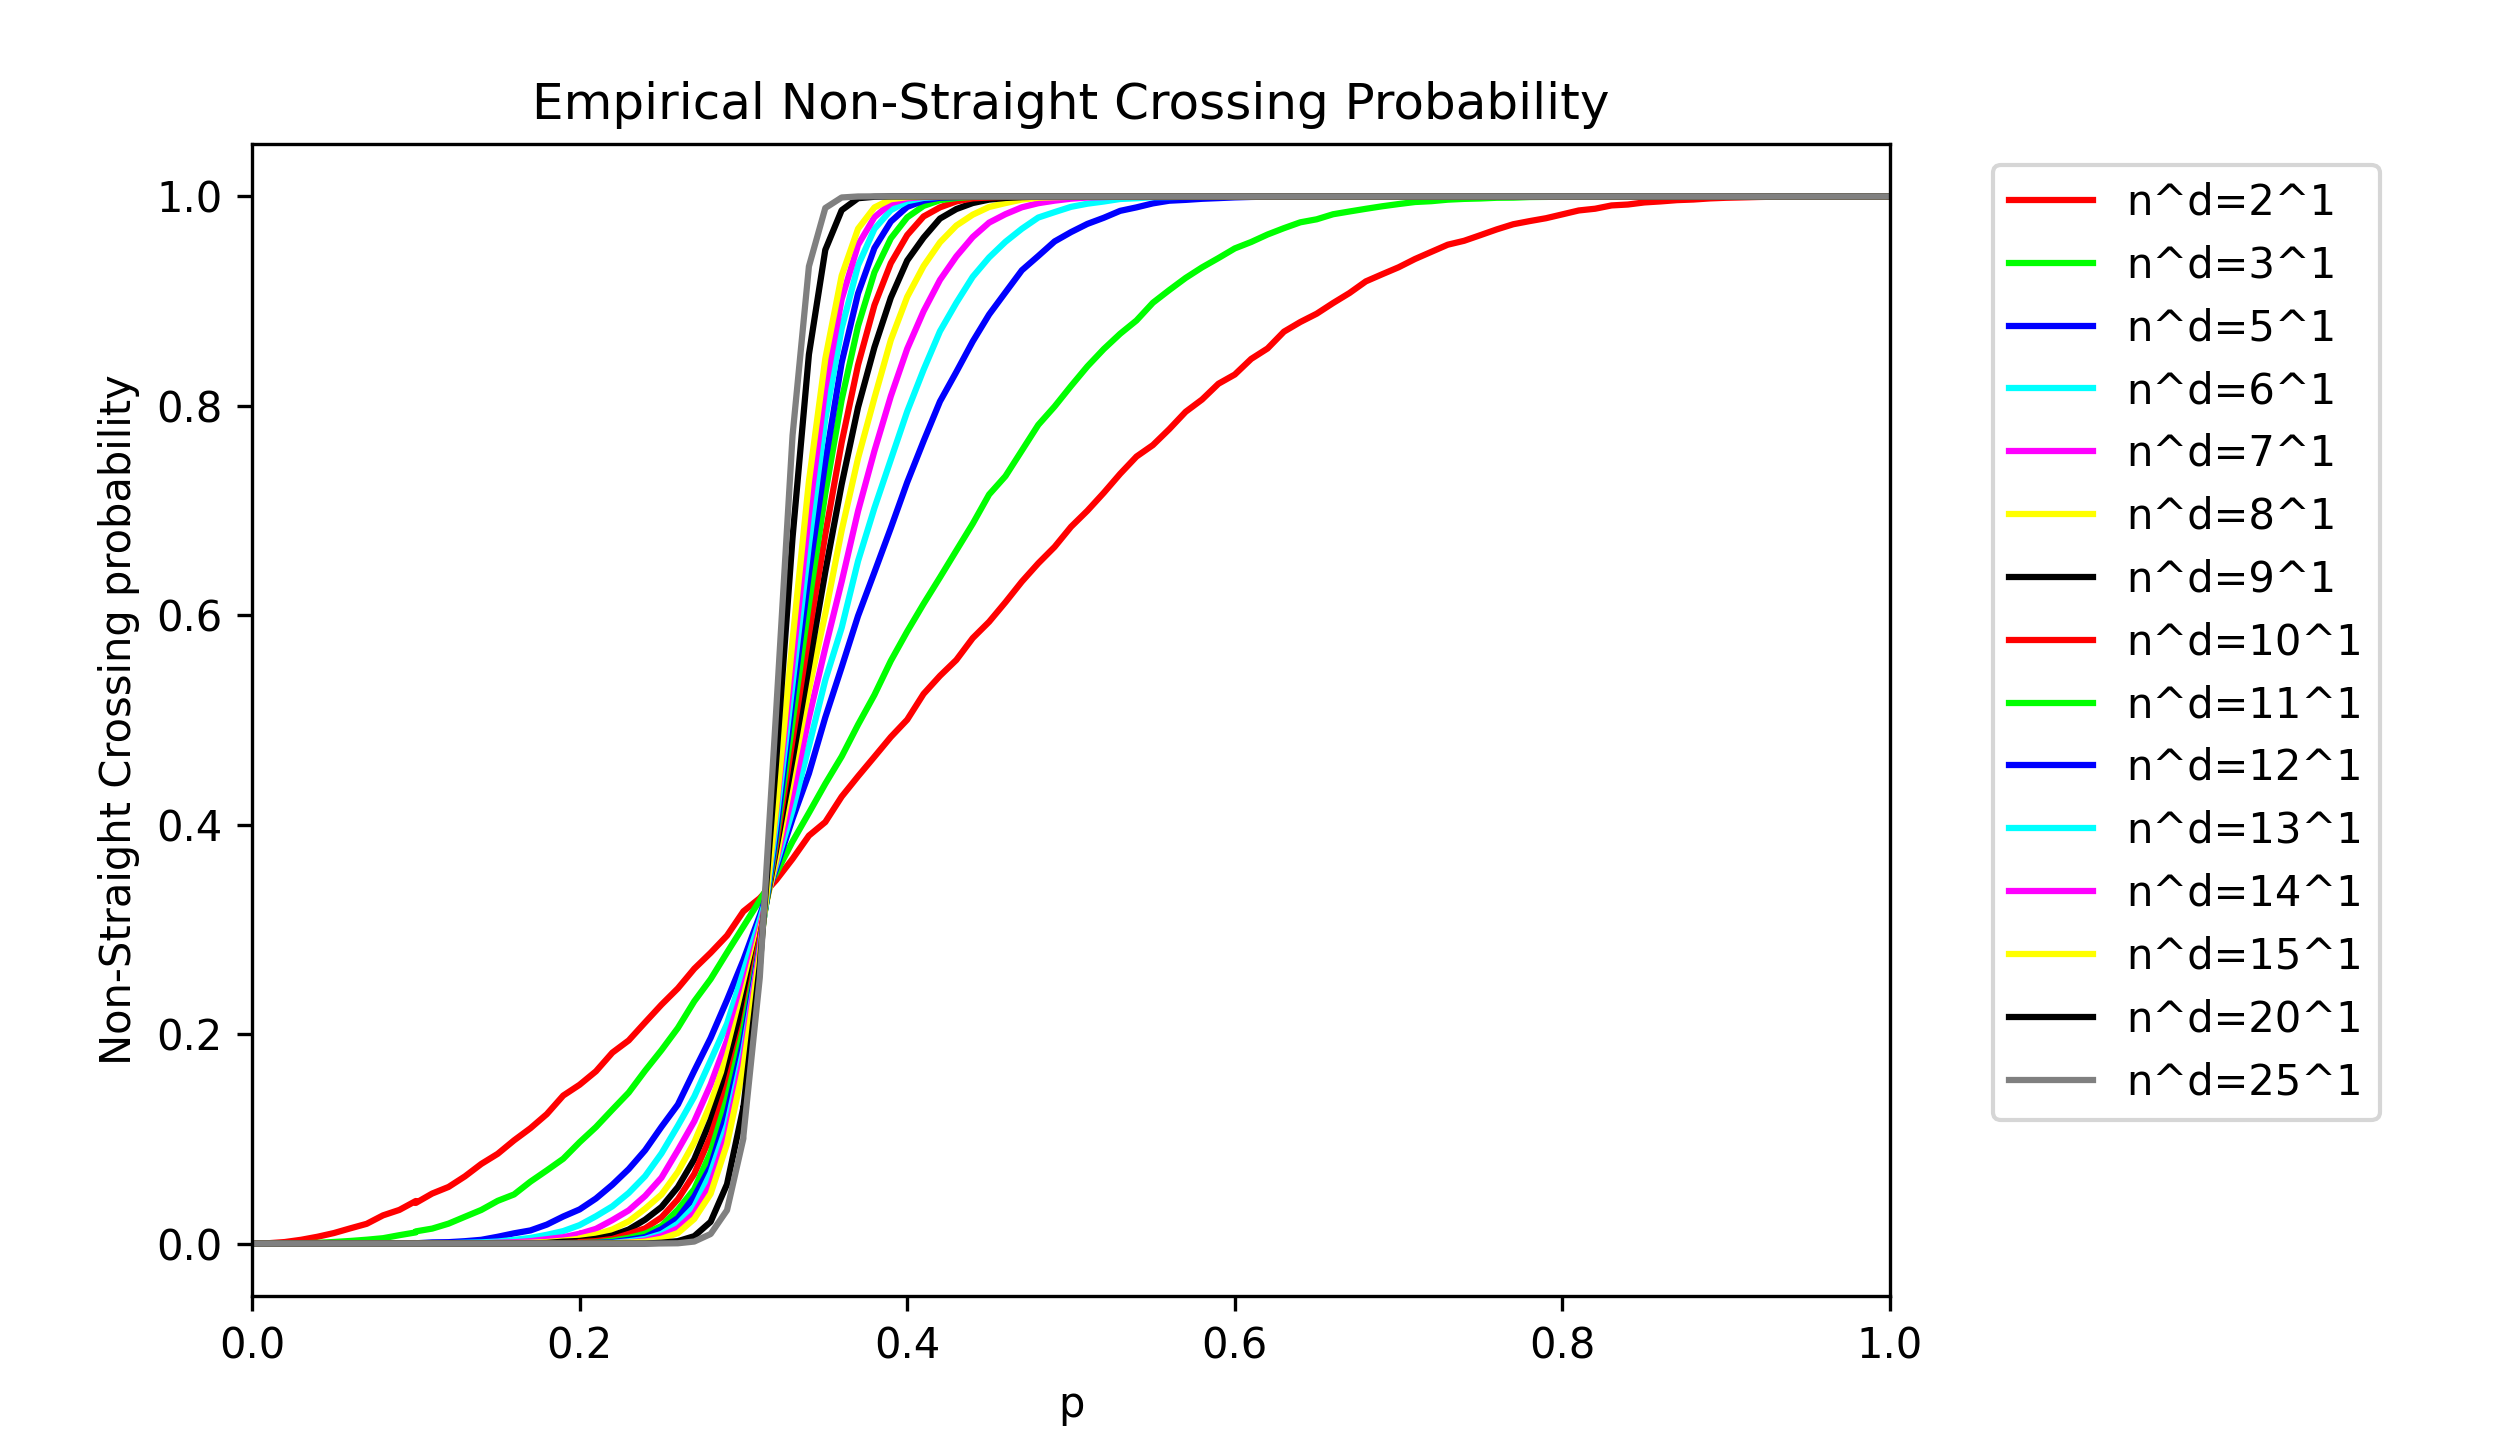
\includegraphics[width=8cm]{crossing_proba_3D_bis}
		\centering
		\captionsetup{justification=centering}
		\caption{Classical Percolation}
	\end{subfigure}
	\hspace{0.04\linewidth}
	\begin{subfigure}{0.45\linewidth}
		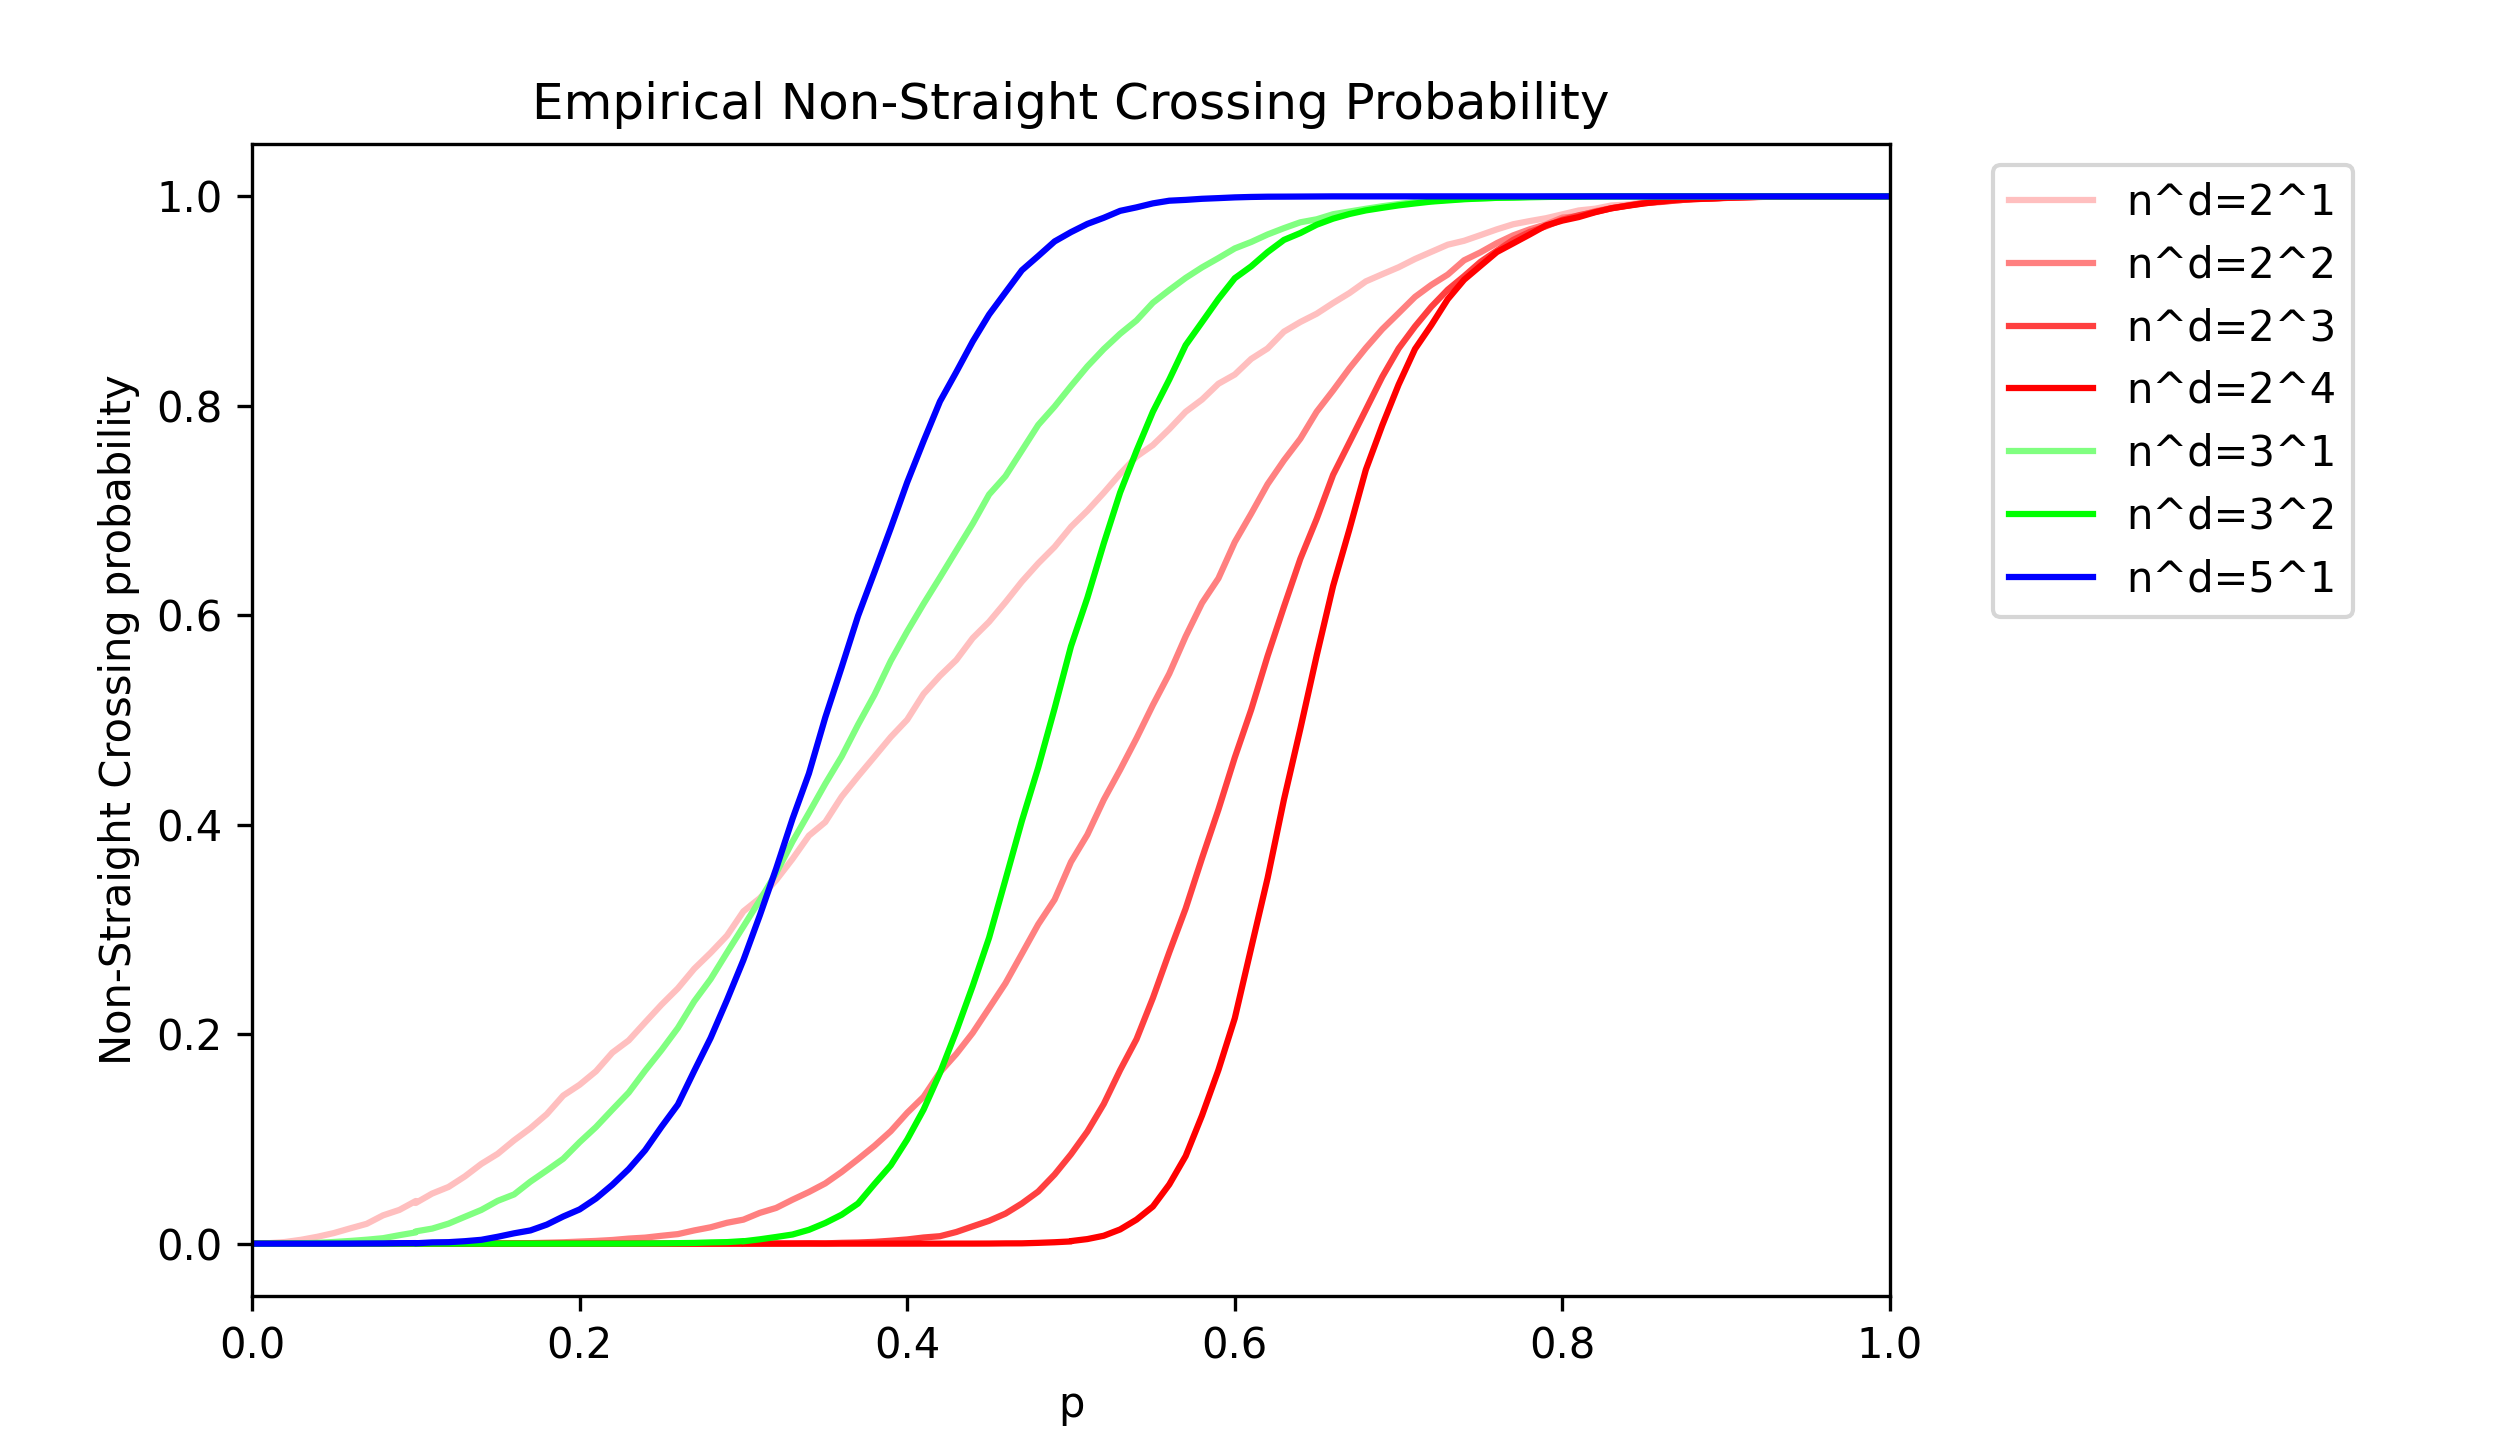
\includegraphics[width=8cm]{crossing_proba_3D}
		\centering
		\captionsetup{justification=centering}
		\caption{Recursive Percolation}
	\end{subfigure}
	\caption{Crossing Probabilities, $D=3$}
	\label{fig:crossingProbabilities3D}
\end{figure}

\subsubsection{Crossings Length}
The length of a straight crossing is always 1.
However, for non-straight and semi-straight crossings, it is less clear.
We study this numerically.

As either $d$ or $n$ increases, the average  length of crossings (when existing) increases.
One may conjecture that eventually, the crossing path are fractals with dimension greater than one (this would agree with a crossing length diverging to infinity).

Semi-straight crossings are on average shorter than non-straight ones (but are less likely to occur).
The average crossing length behaviours are similar for $D=2$ and $D=3$ (see fig. \ref{fig:crossingLengths}).

\begin{figure}[!h]
	\begin{subfigure}{0.45\linewidth}
		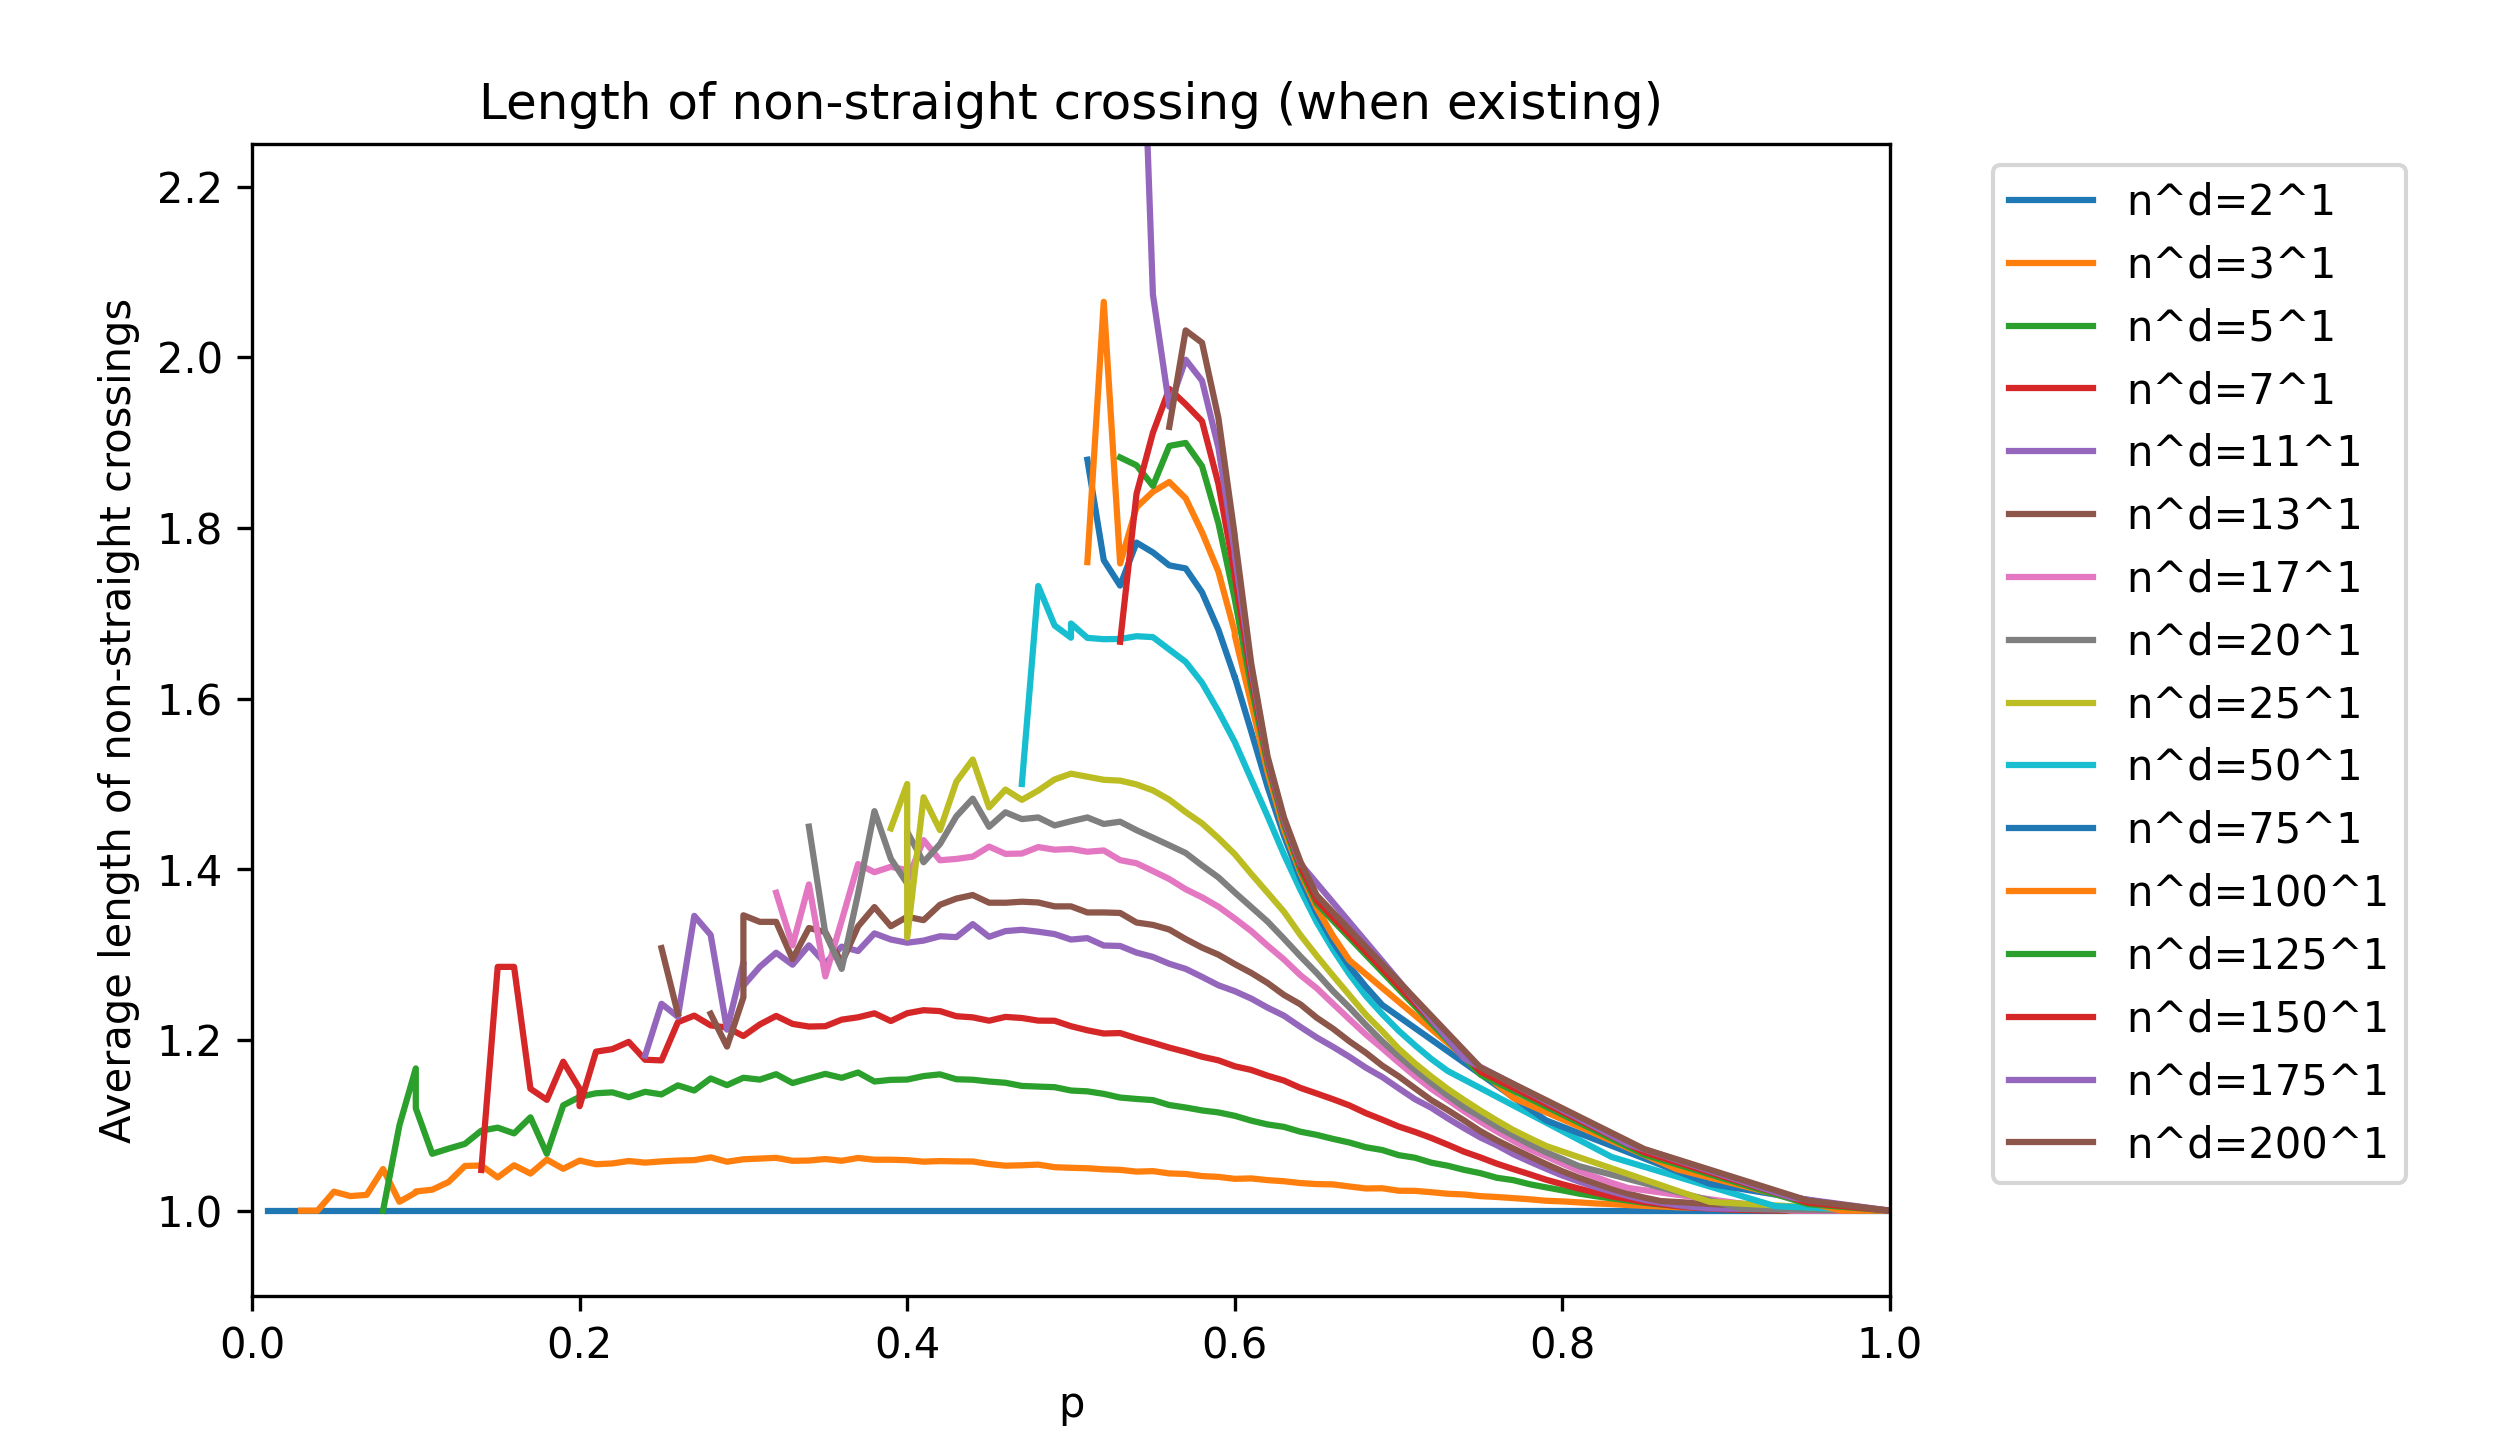
\includegraphics[width=8cm]{crossing_length_2D_ter}
		\centering
		\captionsetup{justification=centering}
		\caption{Classical Percolation, $D=2$}
	\end{subfigure}
	\hspace{0.04\linewidth}
	\begin{subfigure}{0.45\linewidth}
		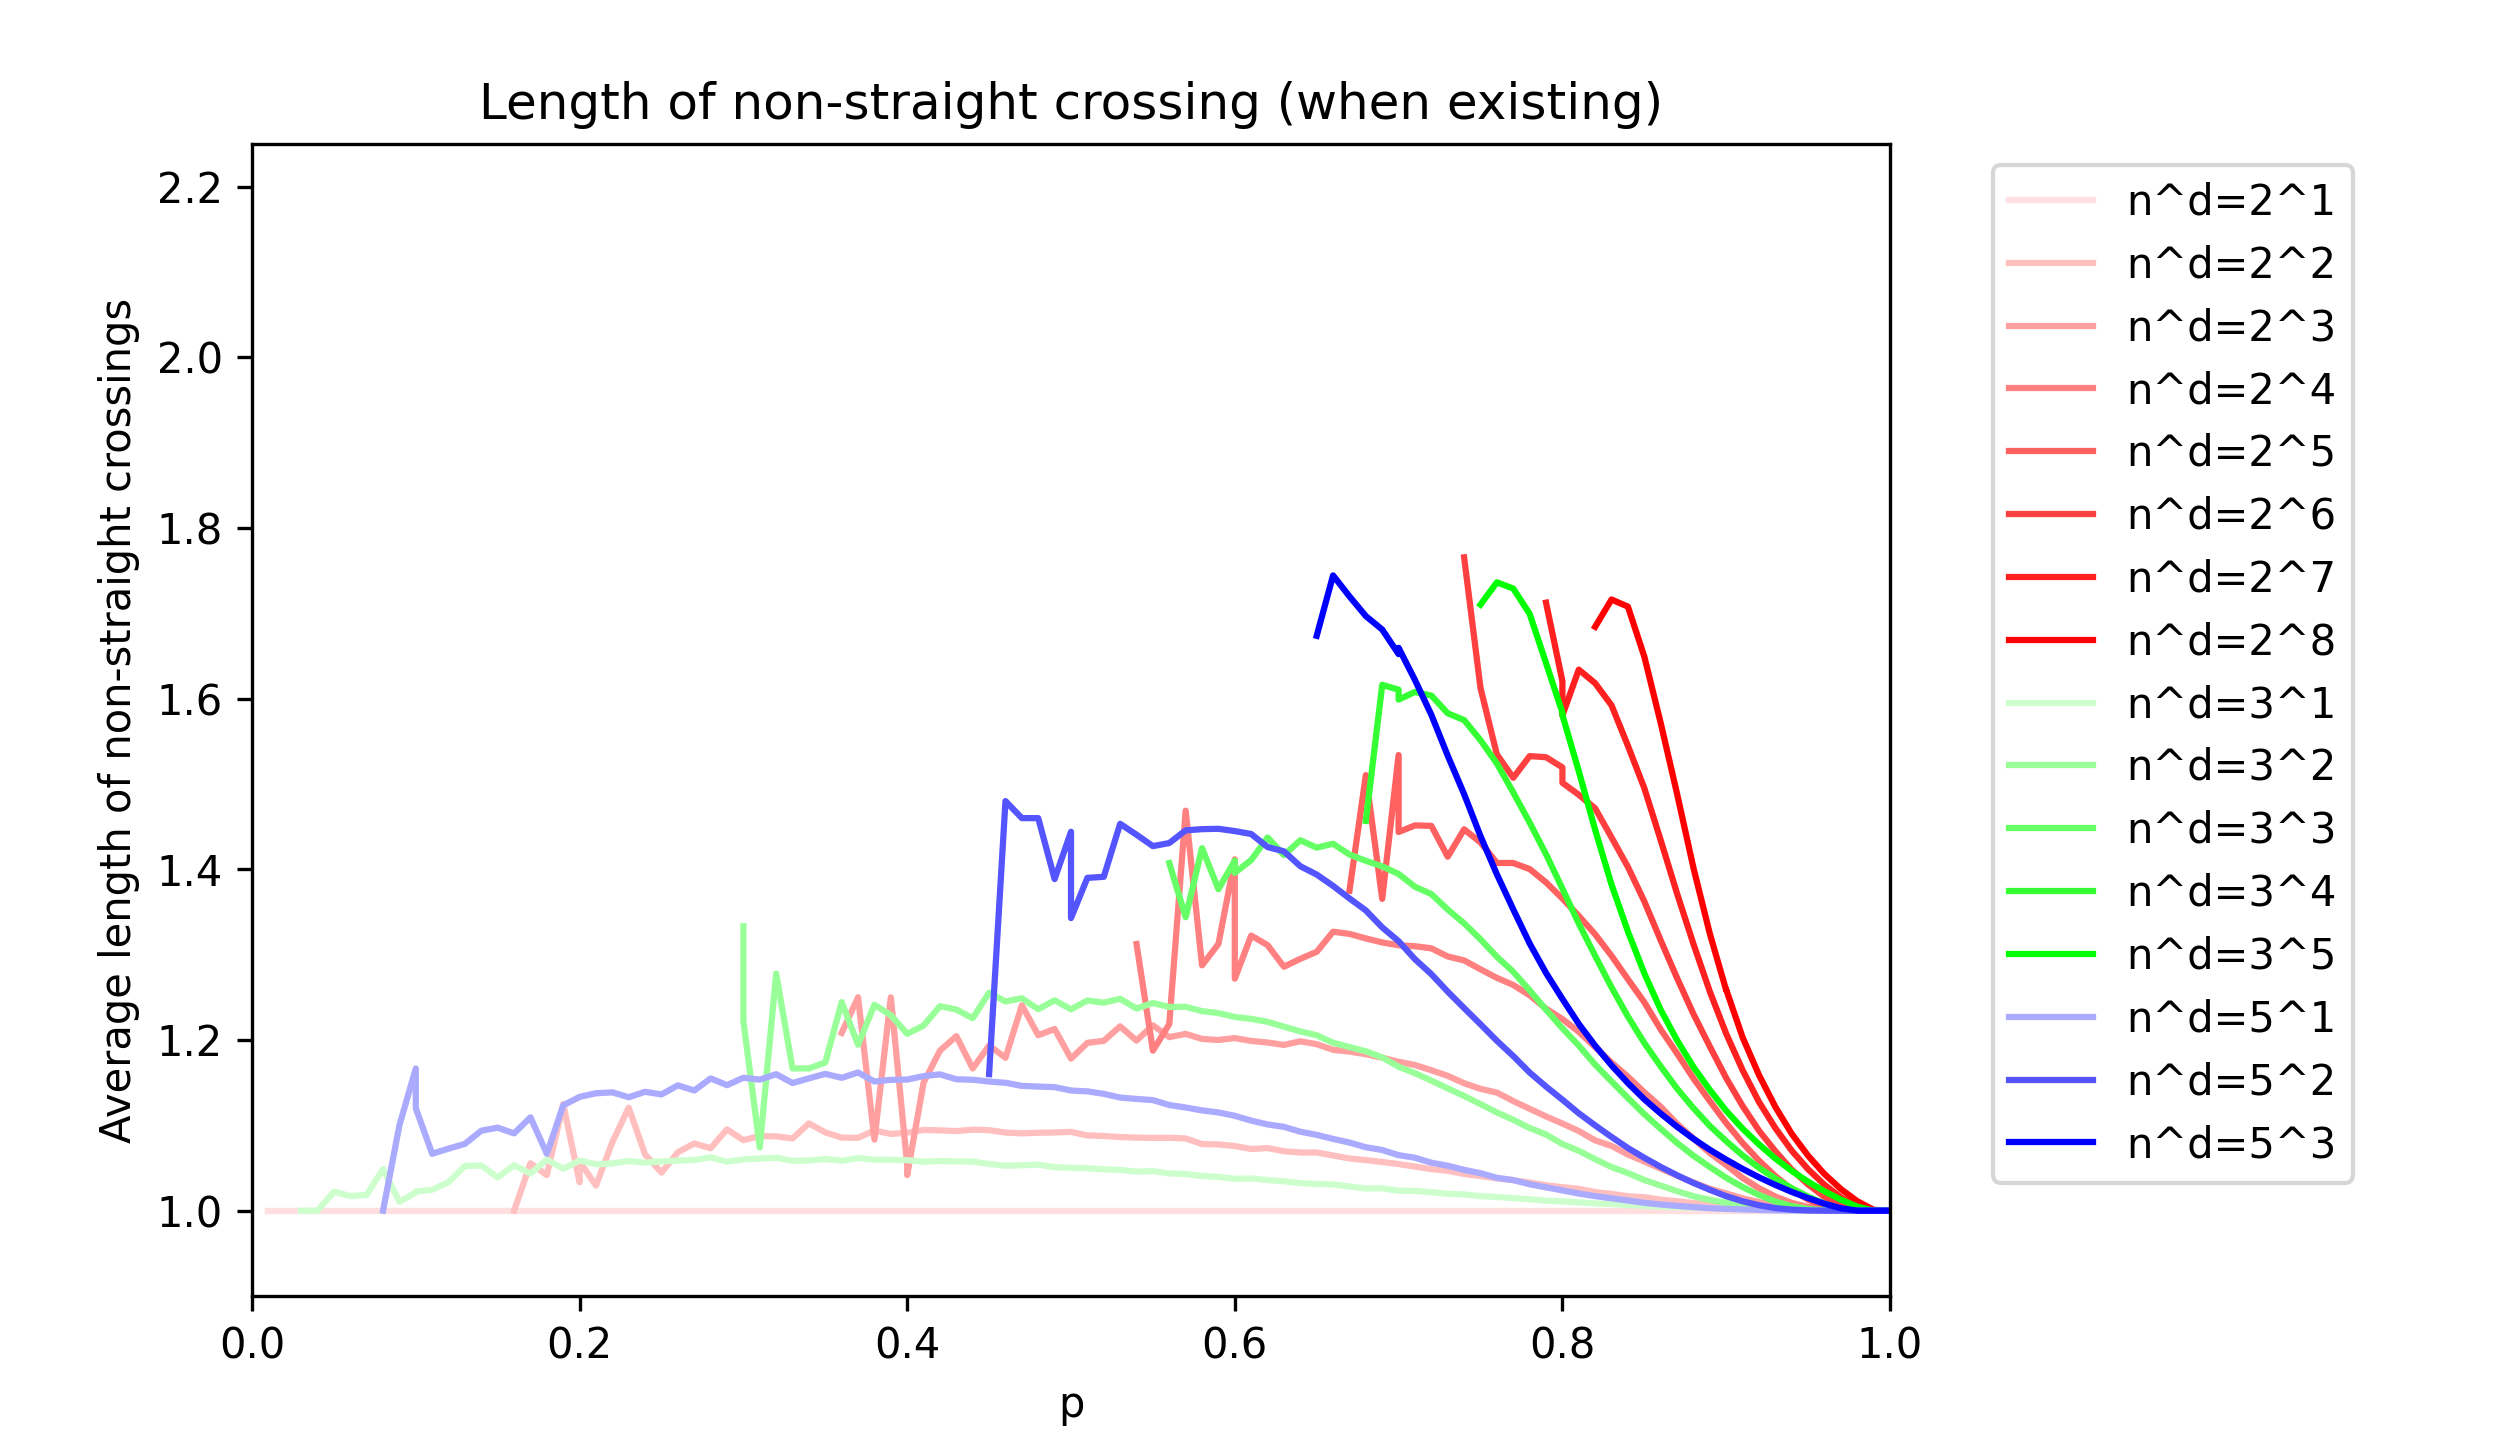
\includegraphics[width=8cm]{crossing_length_2D}
		\centering
		\captionsetup{justification=centering}
		\caption{Recursive Percolation, $D=2$}
	\end{subfigure}

	\begin{subfigure}{0.45\linewidth}
		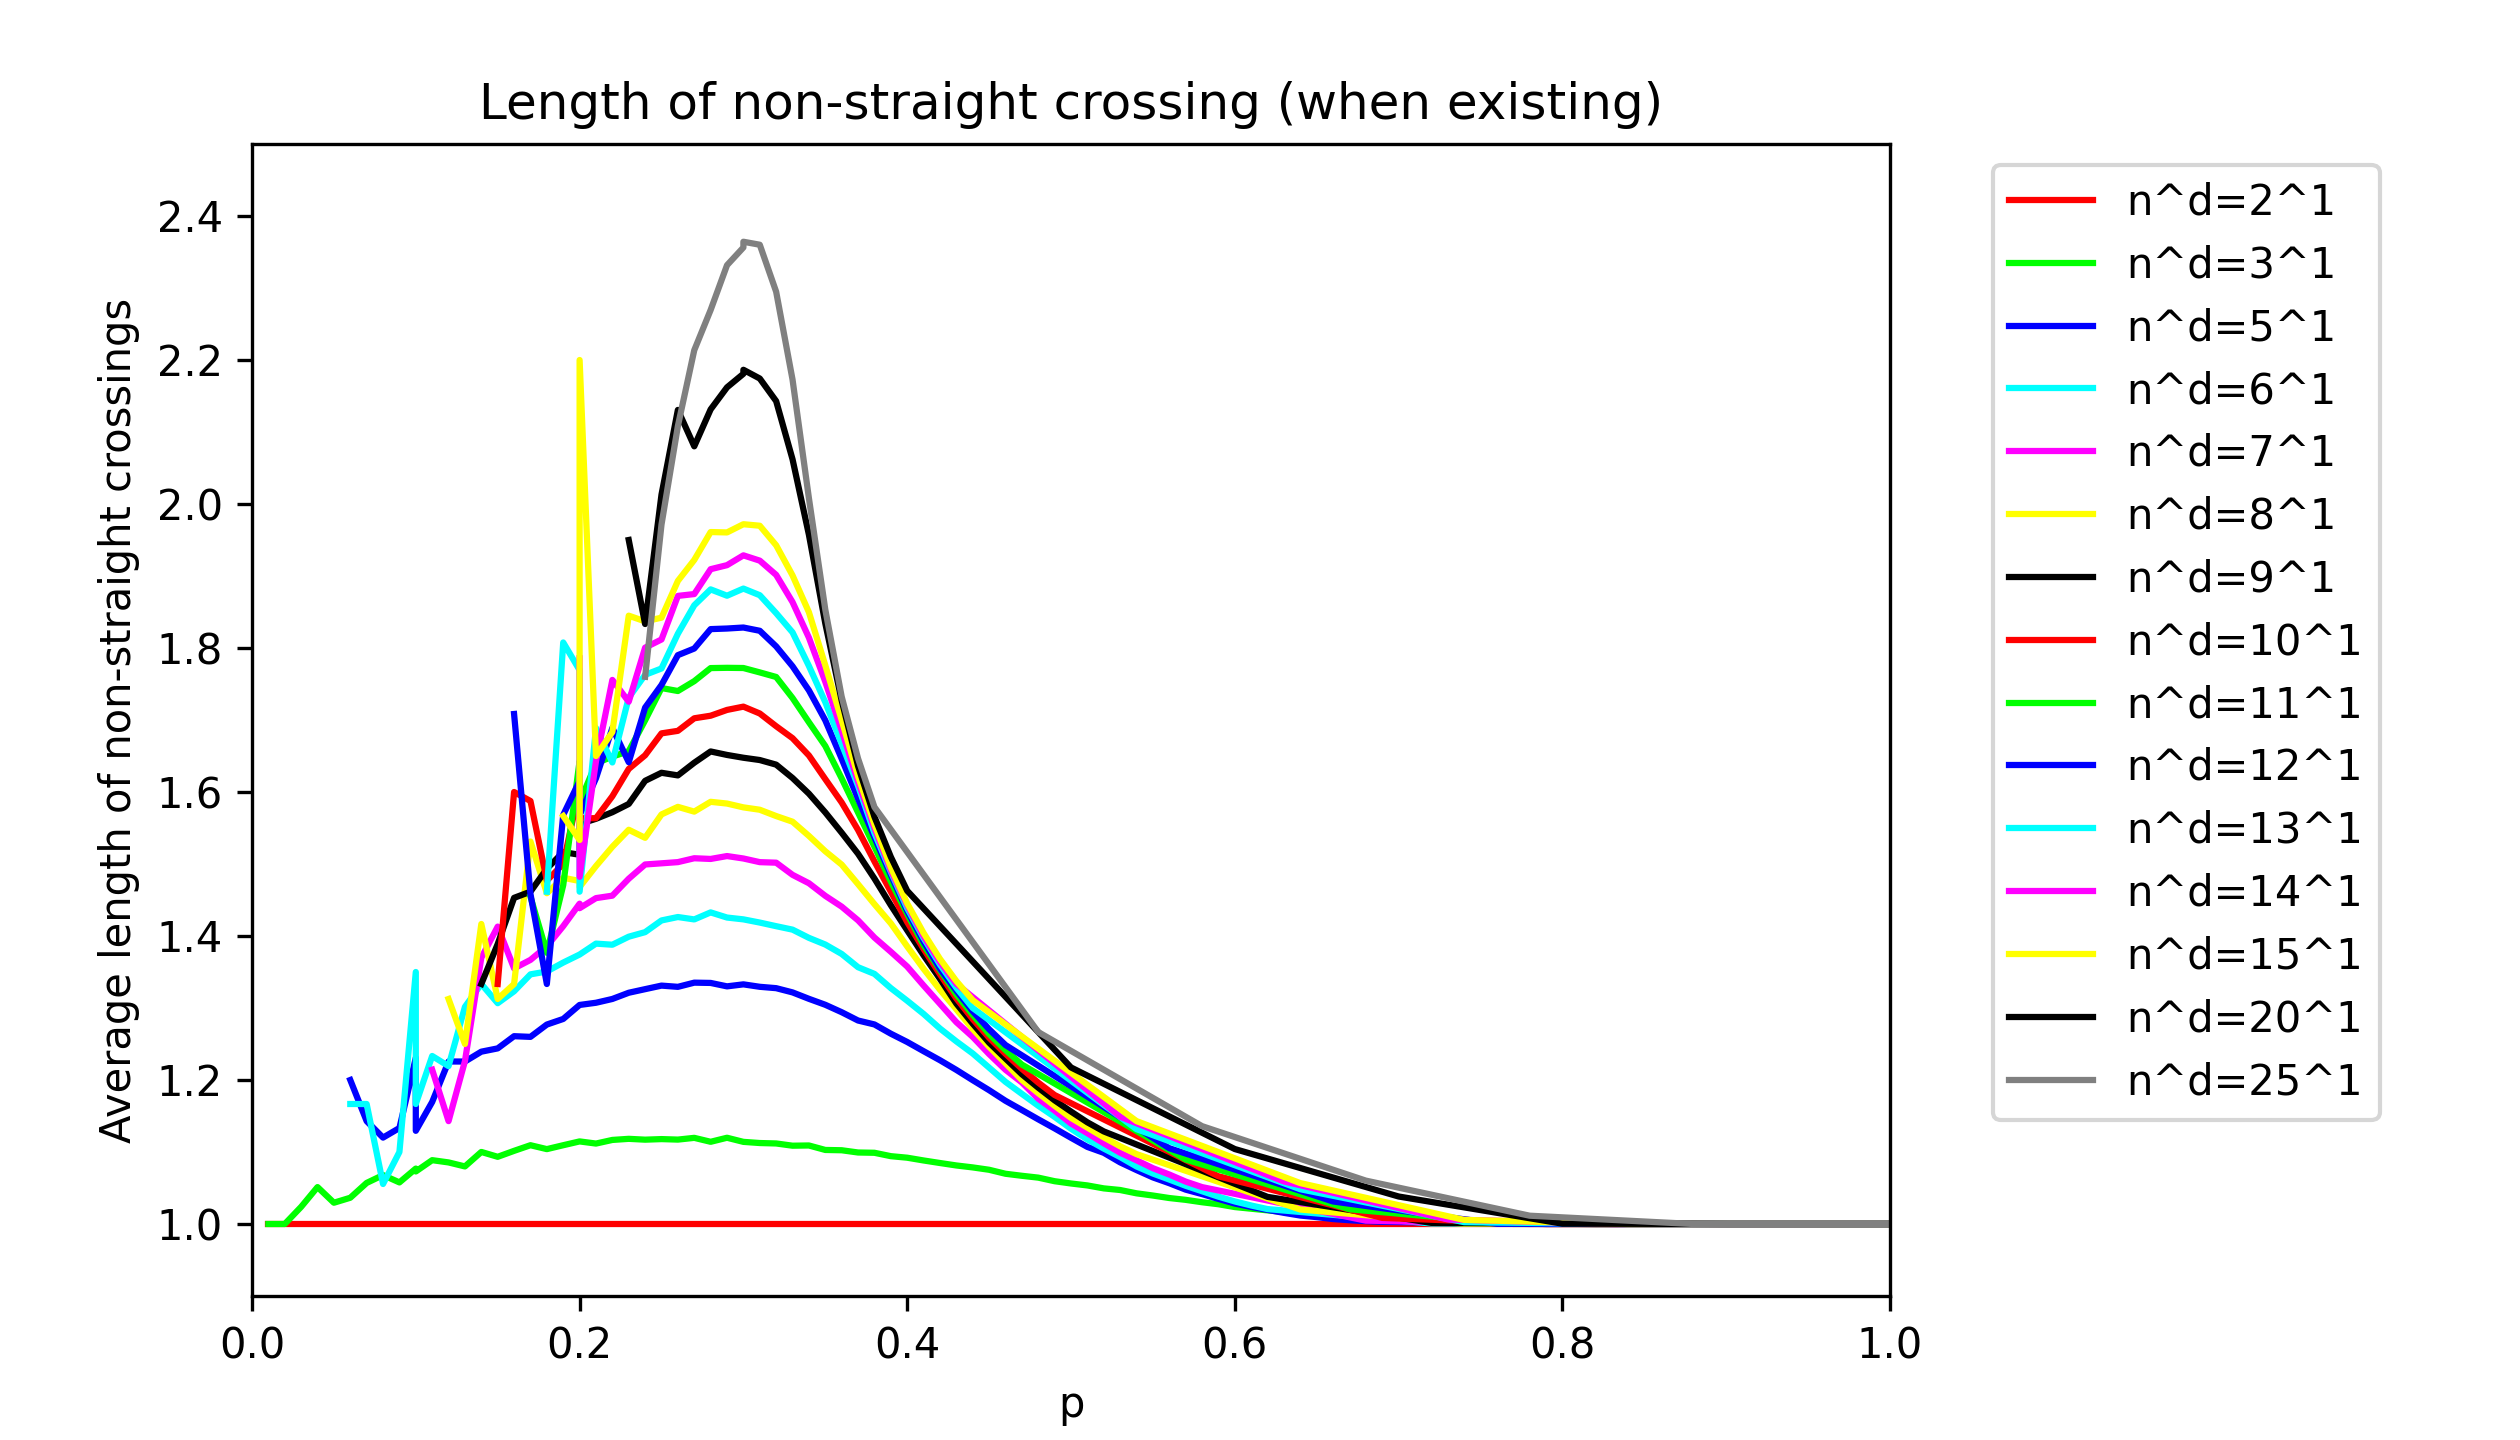
\includegraphics[width=8cm]{crossing_length_3D_bis}
		\centering
		\captionsetup{justification=centering}
		\caption{Classical Percolation, $D=3$}
	\end{subfigure}
	\hspace{0.04\linewidth}
	\begin{subfigure}{0.45\linewidth}
		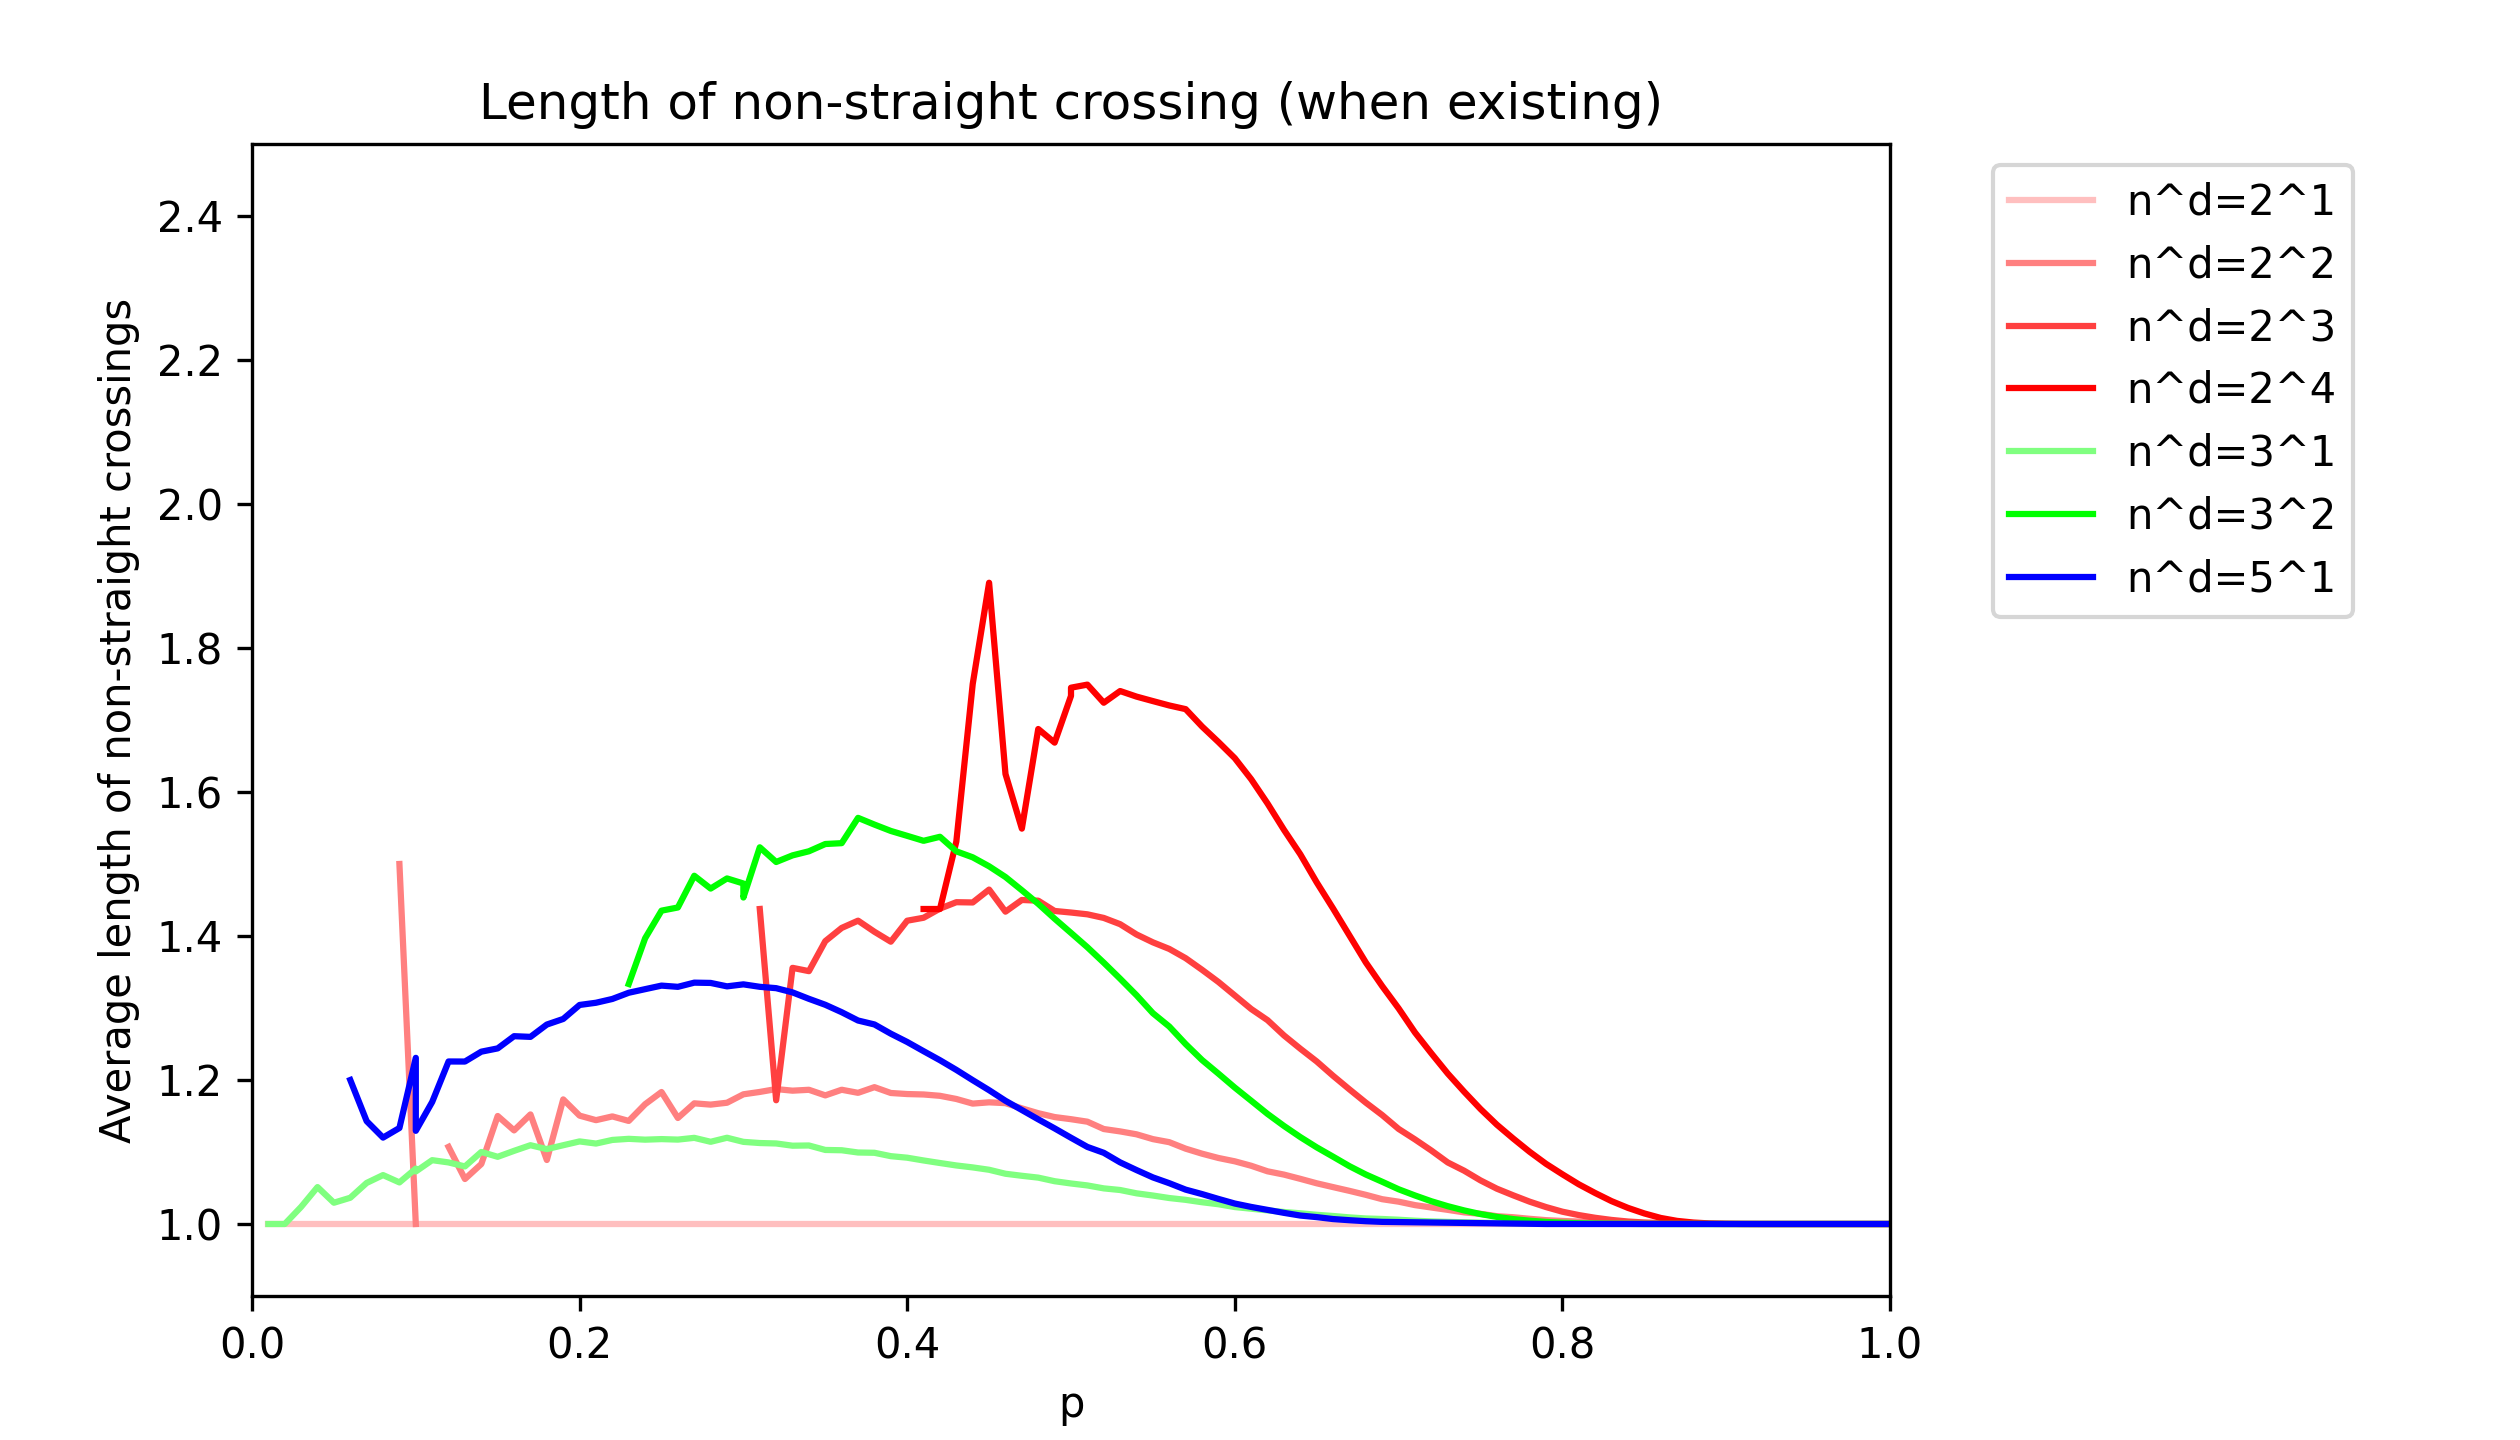
\includegraphics[width=8cm]{crossing_length_3D}
		\centering
		\captionsetup{justification=centering}
		\caption{Recursive Percolation, $D=3$}
	\end{subfigure}

	\caption{Crossings average lengths on percolation (non-straight case).\\
	The oscillations for $p$ small come from the fact that for small values of $p$, very few crossings are found (even out of 50000 simulations). Therefore, the average is taken over fewer values, and we end-up with more noise.}
	\label{fig:crossingLengths}
\end{figure}

%\subsubsection{Crossings Dimension}

\subsection{Percolation Complement Crossings}
We turn our interest to crossings on the complement $P^C = \left[ 0,1 \right]^D \setminus P$ for a recursive percolation $P \sim \text{Perc}^D(n,p,\infty)$.

\begin{figure}[!h]
	\centering
	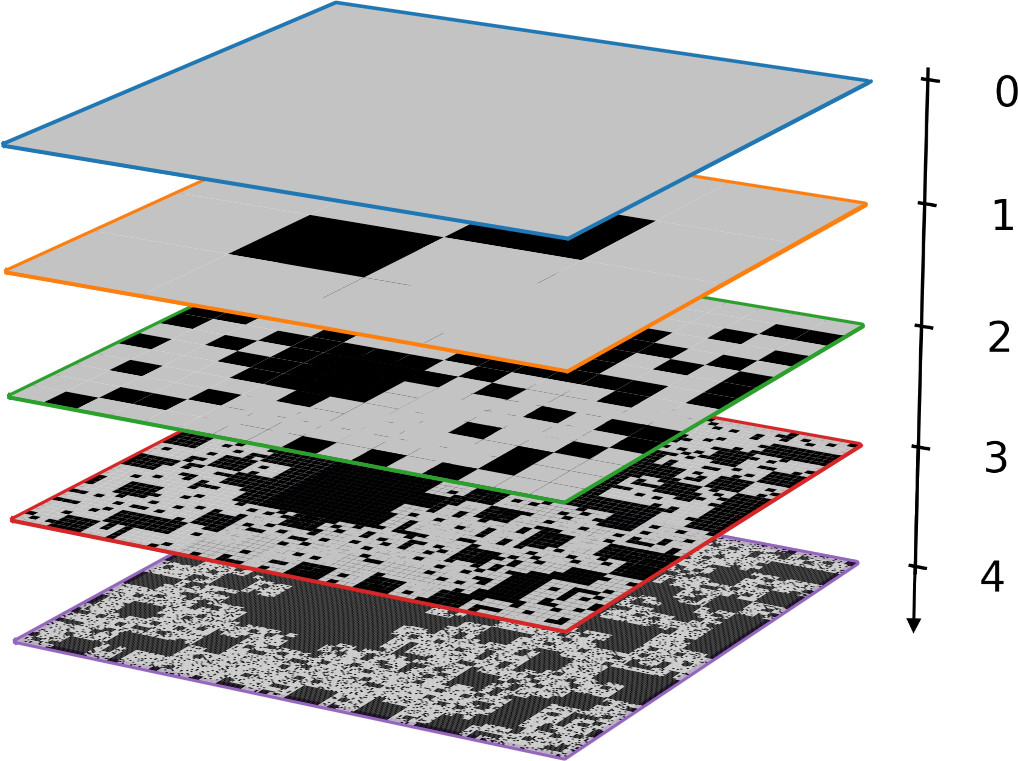
\includegraphics[width=10cm]{recursive_percolation_complement}
	\caption{Recursive Percolation Complement\\($n=4, d=4, p=0.8$)}
	\label{fig:recursivePercolationComplement}
\end{figure}

\subsubsection{Complement Crossings Probability}
Again, we will first be interested in the probability that a crossing exists.

\paragraph{Straight Complement Crossings}
There is a straight crossing on the complement $P^C$ of the percolation if there exists a point $x \in \left[ 0,1 \right]^{D-1}$ such that $\left[ 0,1 \right] \times \{ x \}$  is in $P^C$, i.e. do not intersect with $P$.

The following result is inspired from \cite[p.309 b.(1)]{Chayes_1988} and \cite[p.215]{Mandelbrot_1982}.
Suppose $x = (x_2,\dots,x_D)$ with $x_i \neq \nicefrac{j_i}{n^k} \text{ for } j_i \in \llbracket 0,n^k \rrbracket$\footnote{Writing $\llbracket a,b \rrbracket$ for $\Z \cap \left[ 0,n^d \right]$.}.
Then if $p \leq \nicefrac{1}{n}$ we have that almost surely, $P$ has a complement crossing along $\left[ 0,1 \right] \times \{ x \}$.
This is in fact equivalent to 
$$\mathbb{P}\left( \left( P \cap \left[ 0,1 \right] \times \{ x \} \right) = \emptyset \right) = 1 .$$
\begin{proof}
	Let $x \neq \left( \frac{j_2}{n^k},\dots,\frac{j_D}{n^k} \right) \text{ for any } j_i \in \llbracket 0,n^k \rrbracket$.
	The number of intervals of the form $\left[ \frac{j_1-1}{n^k},\frac{j_1}{n^k} \right] \times \{ x \}$ still in the percolation at depth $k$ is a branching process in which each interval has $np$ offsprings.
	Thus, the branching process dies out almost surely if $np \leq 1$, i.e. $p \leq \nicefrac{1}{n}$.
	When the process dies, we have $\left[ 0,1 \right] \times \{ x \} \subseteq P^C$, so there is a crossing in the complement of $P$.
\end{proof}

\paragraph{Non-Straight Complement Crossings}
There will be a non-straight crossing in the percolation complement almost surely if $p \leq \frac{1}{\sqrt[2(D-1)]{n}}$\footnote{Where $\sqrt[2(D-1)]{n}$ is the $2(D-1)^{th}$ root of $n$.}.
The following proof extends techniques from \cite[p.310 b.(2)]{Chayes_1988}.
\begin{proof}\label{prf:nonStraightComplementCrossigs}
	This time, take $x = \left( \frac{j_2}{n^k},\dots,\frac{j_D}{n^k} \right) \text{ with } j_i \in \llbracket 1,n^k-1 \rrbracket$, $x_i = \nicefrac{j_i}{n^k}$.
	Call a segment $\left[ \frac{j_1-1}{n^k},\frac{j_1}{n^k} \right] \times \{ x \}$ vacant if any of the $2(D-1)$ cuboids adjacent at the depth $k$ of the percolation have been removed.
	
	Let $Y^k$, be the number of occupied segments of the form $\{ x \} \times \left[ \frac{j_1-1}{n^k},\frac{j_1}{n^k} \right]$ at depth $k$.
	Then $Y^k$, is a branching process in which the mean number of offsprings is $p^{2(D-1)n}$.
	This branching process is almost surely eventually empty if $np^{2(D-1)} \leq 1$, i.e. if $p \leq \frac{1}{\sqrt[2(D-1)]{n}}$.
	
	Suppose the branching process dies at depth $k$.
	Then there are only finitely many points of the form $\left( \nicefrac{j_1}{n^k}, x_2,\dots,x_D \right) \text{ s.t. } j_1 \in \llbracket 1,n^k-1 \rrbracket$.
	It is almost sure that eventually, all the cuboids touching these points will be removed (since they are kept with a probability $p<1$ after each filtration).
	Once this is the case, there is a crossing path from $\left( 0, x_2,\dots,x_D \right)$ to $\left( 1, x_2,\dots,x_D \right)$ that oscillate near the segment $\left[ 0,1 \right] \times \{ x \}$ (see fig. \ref{fig:complementCrossing} for illustrations in two and three dimensions).
\end{proof}

\begin{figure}[!h]
	\vspace{-0.75cm}
	\begin{subfigure}{0.44\linewidth}
		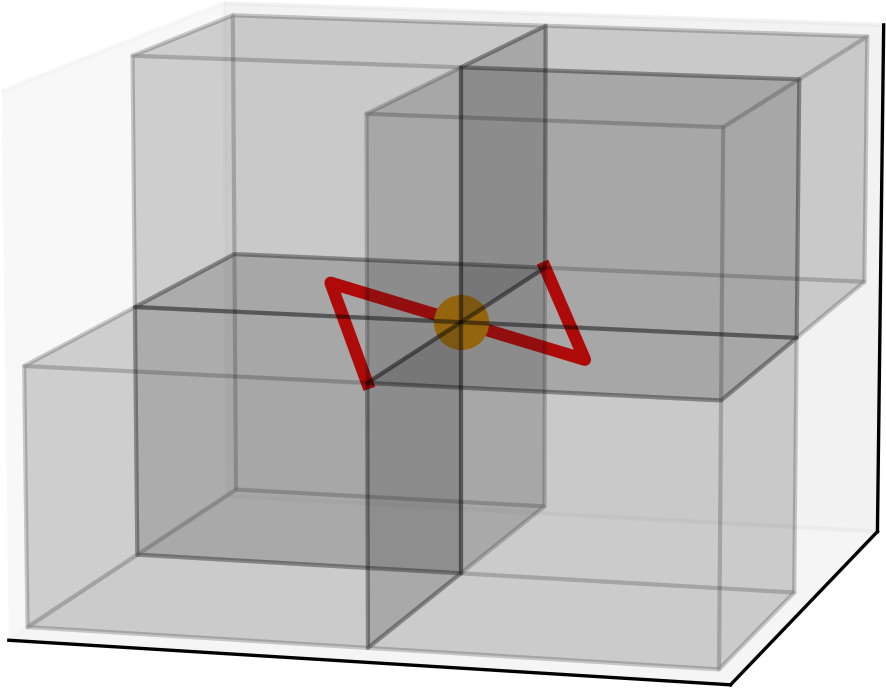
\includegraphics[width=5.25cm]{complement_crossing3D}
		\centering
		\captionsetup{justification=centering}
		\caption{$D = 3$}
		\label{fig:complementCrossing3D}
	\end{subfigure}
	\hspace{0.1\linewidth}
	\begin{subfigure}{0.44\linewidth}
		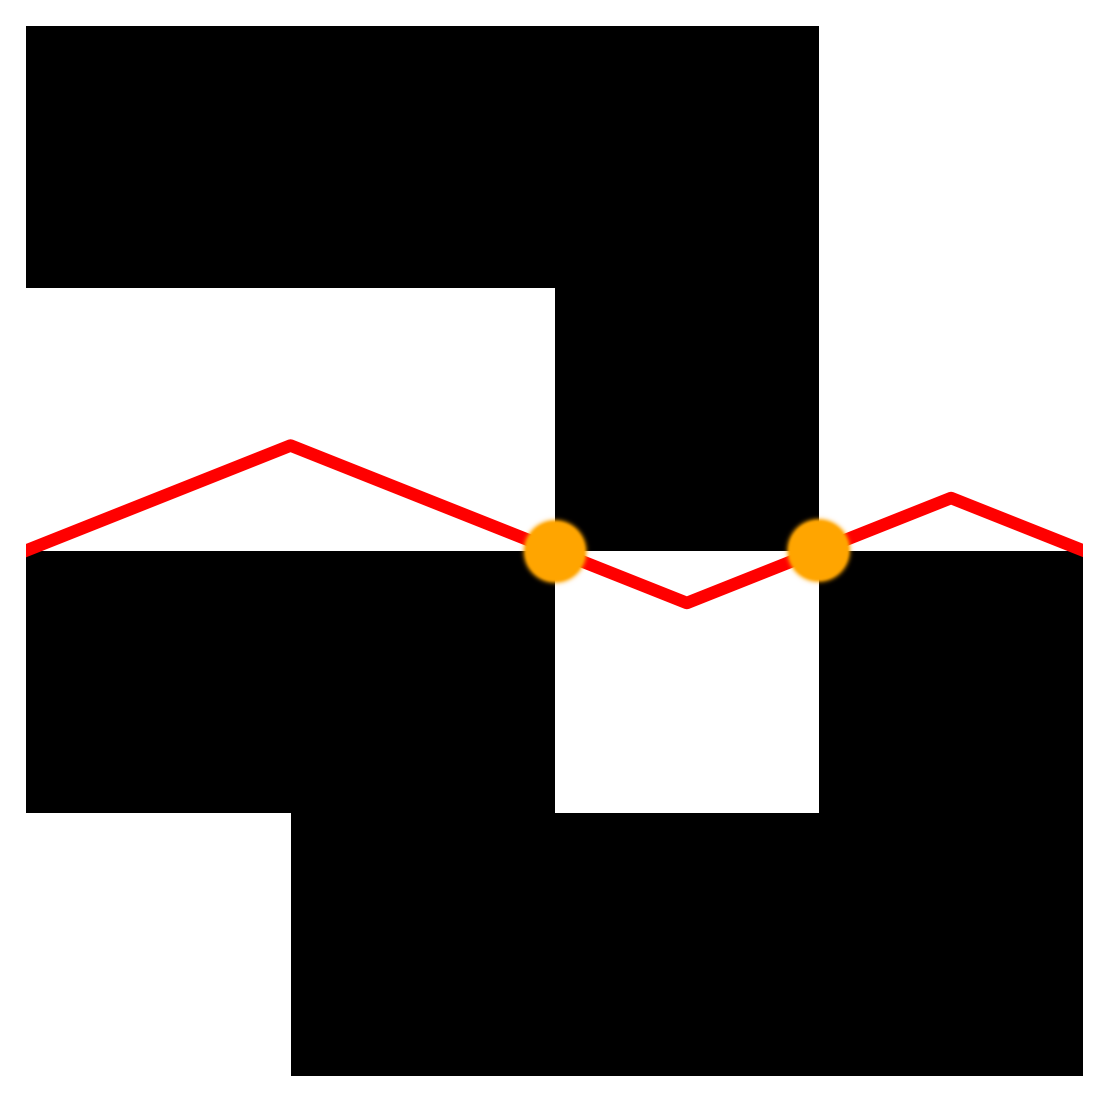
\includegraphics[width=5.25cm]{complement_crossing2D}
		\centering
		\captionsetup{justification=centering}
		\caption{$D = 2$}
		\label{fig:complementCrossing2D}
	\end{subfigure}
	\centering
	\caption{Eventually, the cuboids touching the orange point(s) will be removed and the red path will remain in full within the percolation complement.}
	\label{fig:complementCrossing}
\end{figure}

\paragraph{Numerics}
The crossing probabilities on percolation complement behave similarly as the ones on the percolation: there is a phase transition (this time, from 1 to 0 instead of from 0 to 1 as $p$ increases).
Moreover, the transition shrinks and we can conjecture that eventually, there will only be two regimes.
A further study of this behaviour is left to future work.
Again, all results (we will only show a subset here) are available interactively at \url{https://pauldubois98.github.io/PercolationFractalsStudy/complement_crossings.html}.

\begin{figure}[!h]
	\begin{subfigure}{0.44\linewidth}
		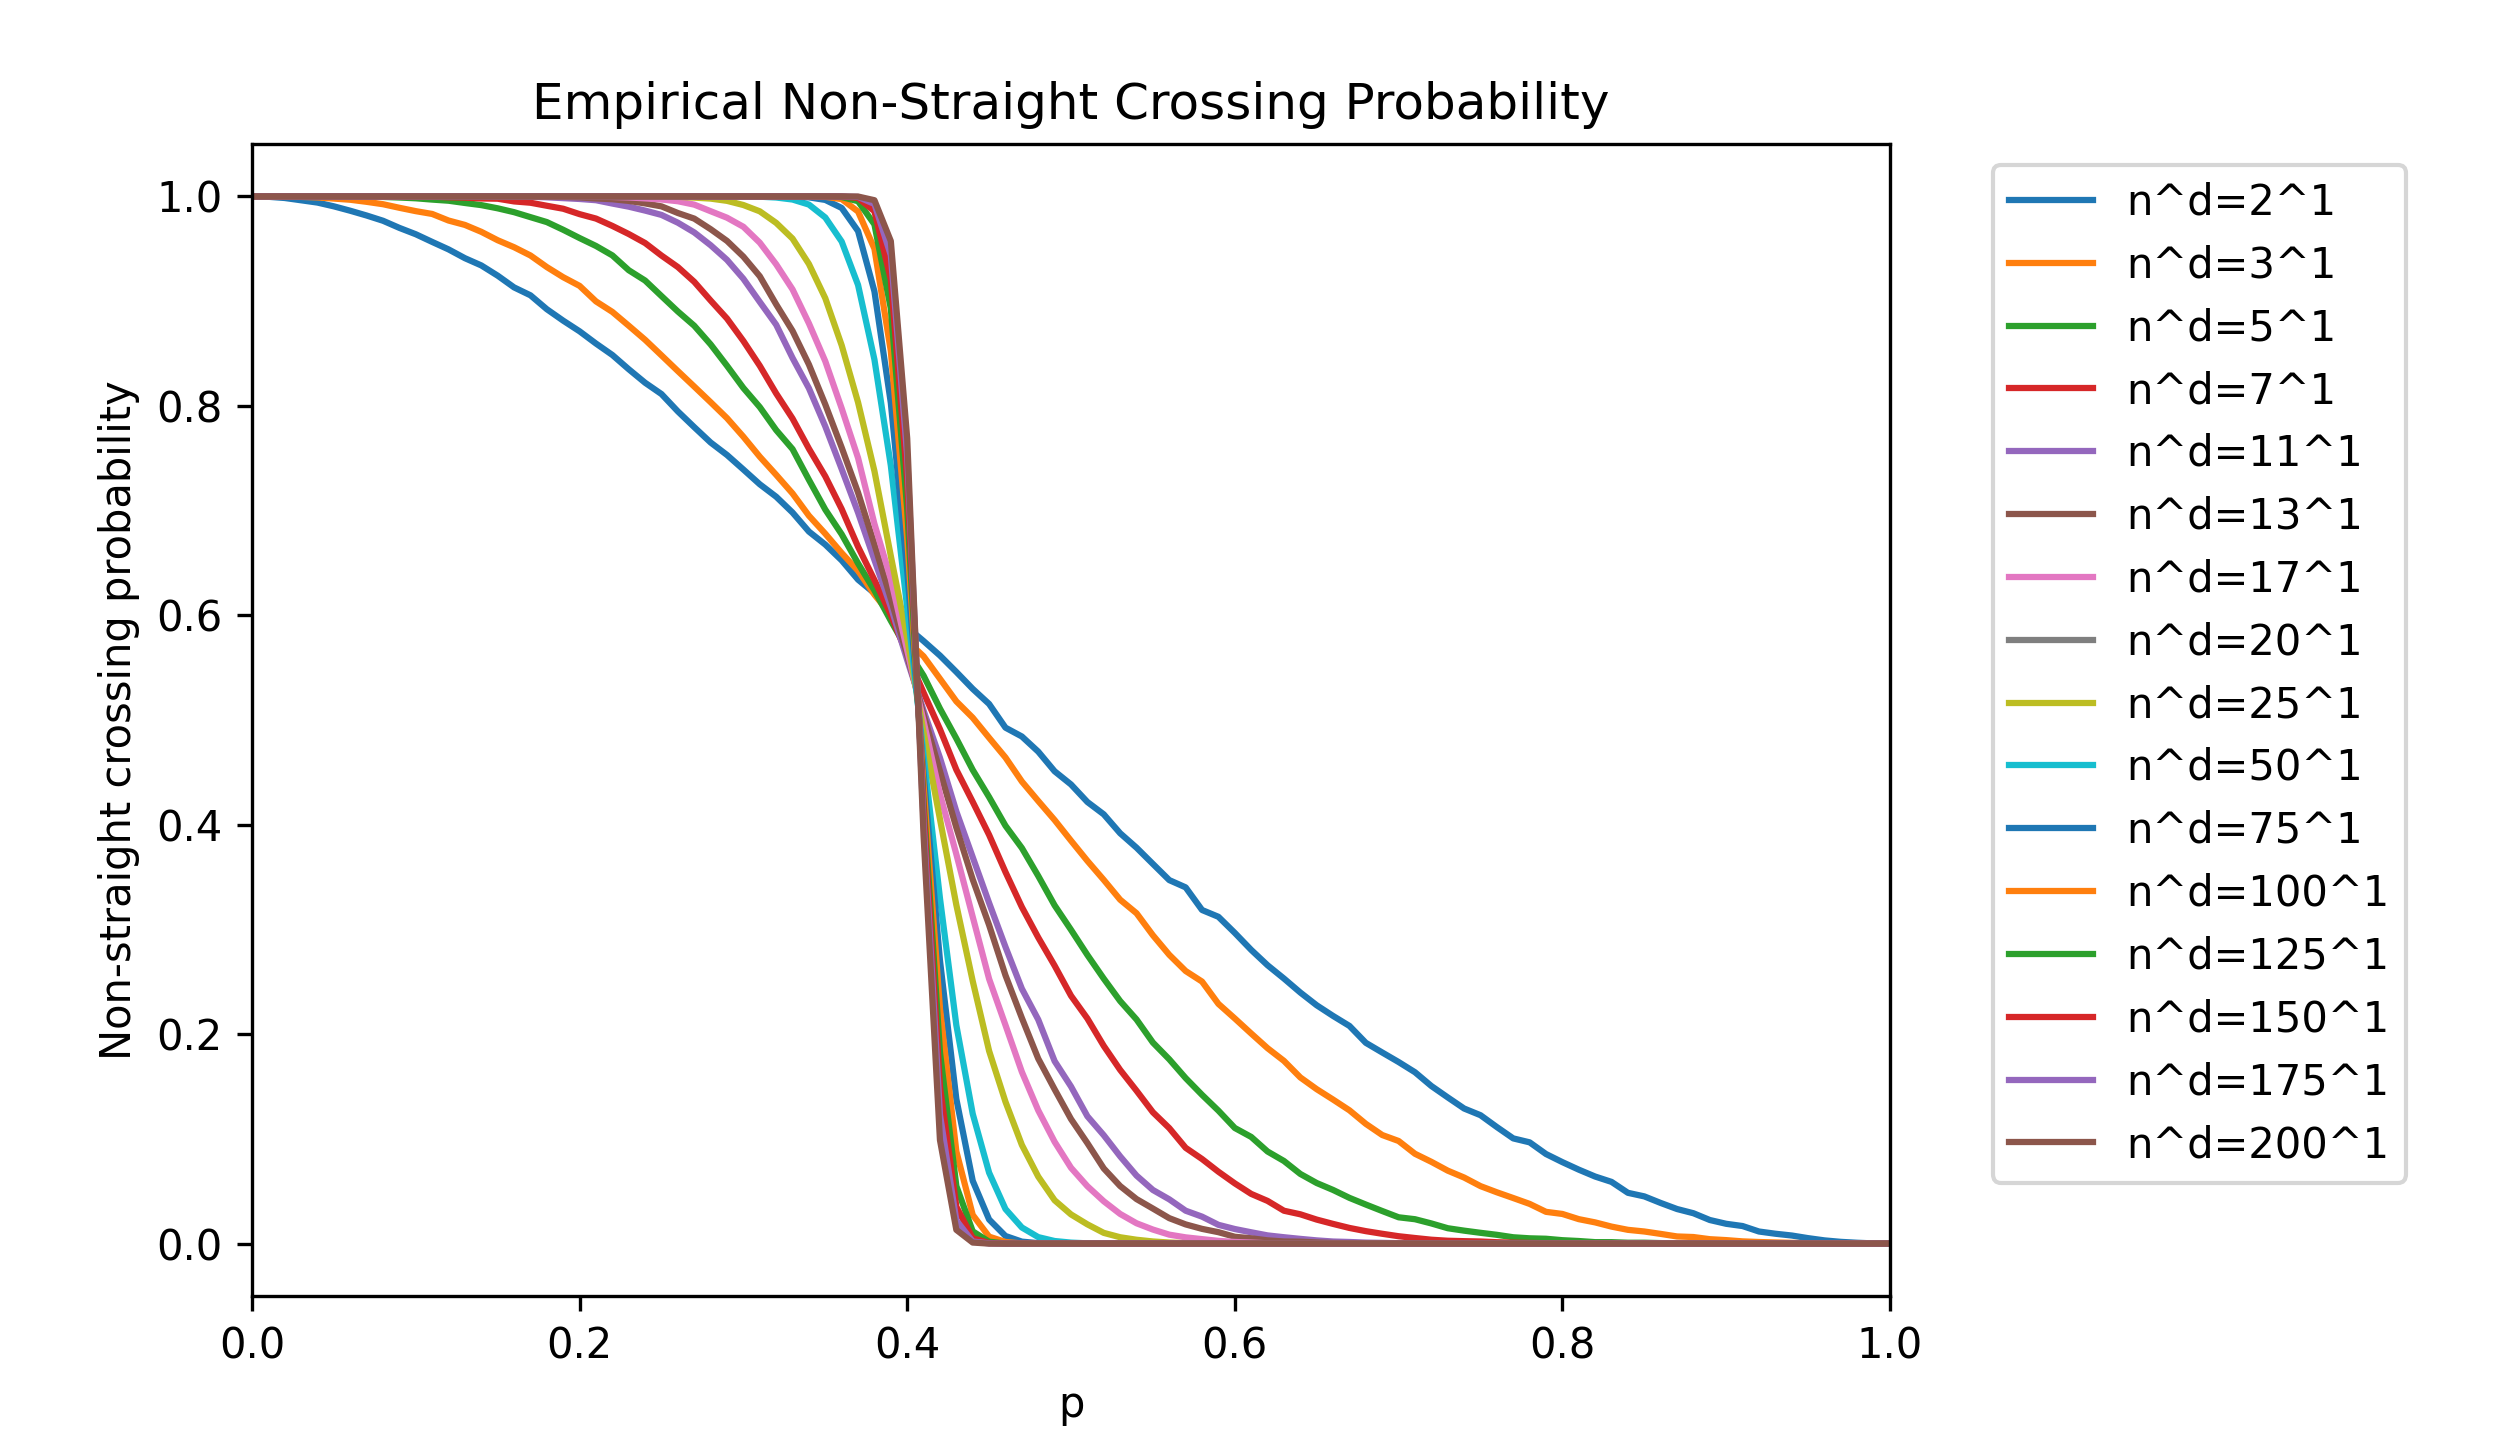
\includegraphics[width=8cm]{complement_crossing_proba_2D_ter}
		\centering
		\captionsetup{justification=centering}
		\caption{Classical Percolation}
	\end{subfigure}
	\hspace{0.1 \linewidth}
	\begin{subfigure}{0.44\linewidth}
		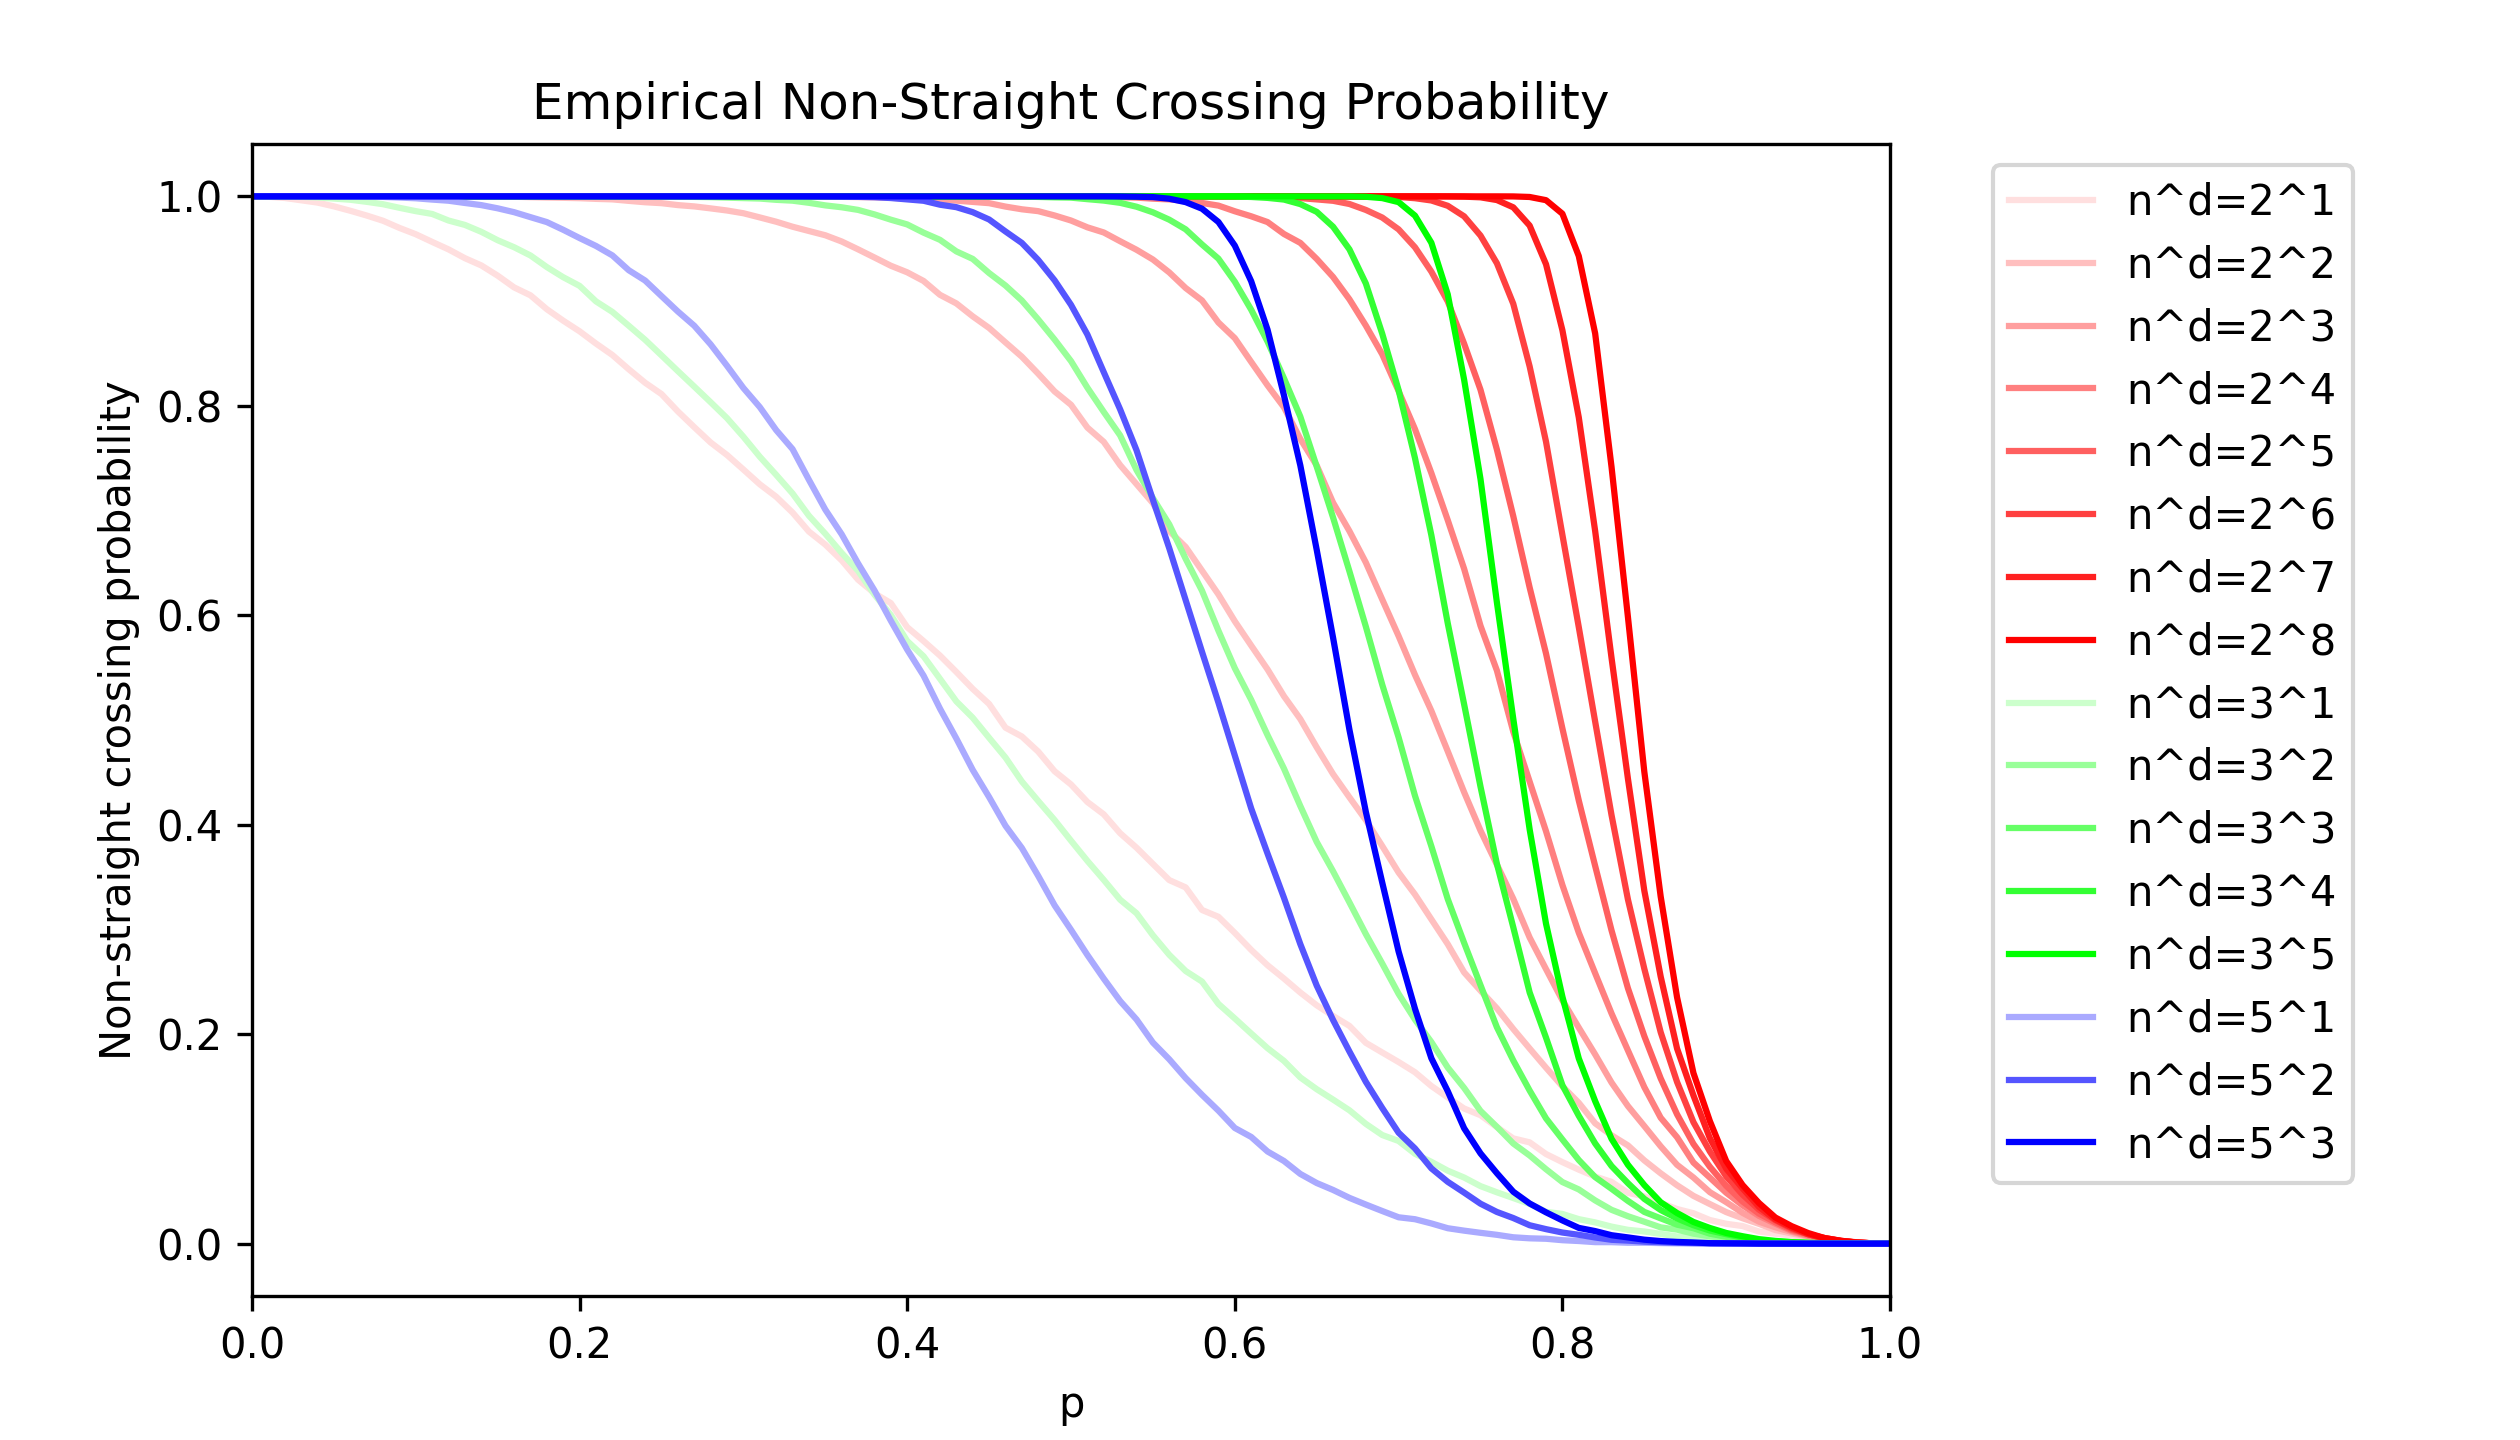
\includegraphics[width=8cm]{complement_crossing_proba_2D}
		\centering
		\captionsetup{justification=centering}
		\caption{Recursive Percolation}
	\end{subfigure}
	\caption{Crossing probability on percolation complement (non-straight case).}
	\label{fig:crossingComplementProbabilities}
\end{figure}

\subsubsection{Crossings Length}
For classical percolations ($d=1$, $n \to \infty$), the simulations show very similar result to the ones of crossings on the percolation (but symmetric about the axis $p=0.5$).
However, for recursive percolations, the behaviour is very different: crossings length do not increase much, even when $p$ is large\footnote{So the percolation complement is small set.}.
The further study of this behaviour is left to future work.

\begin{figure}[!h]
	\begin{subfigure}{0.44\linewidth}
		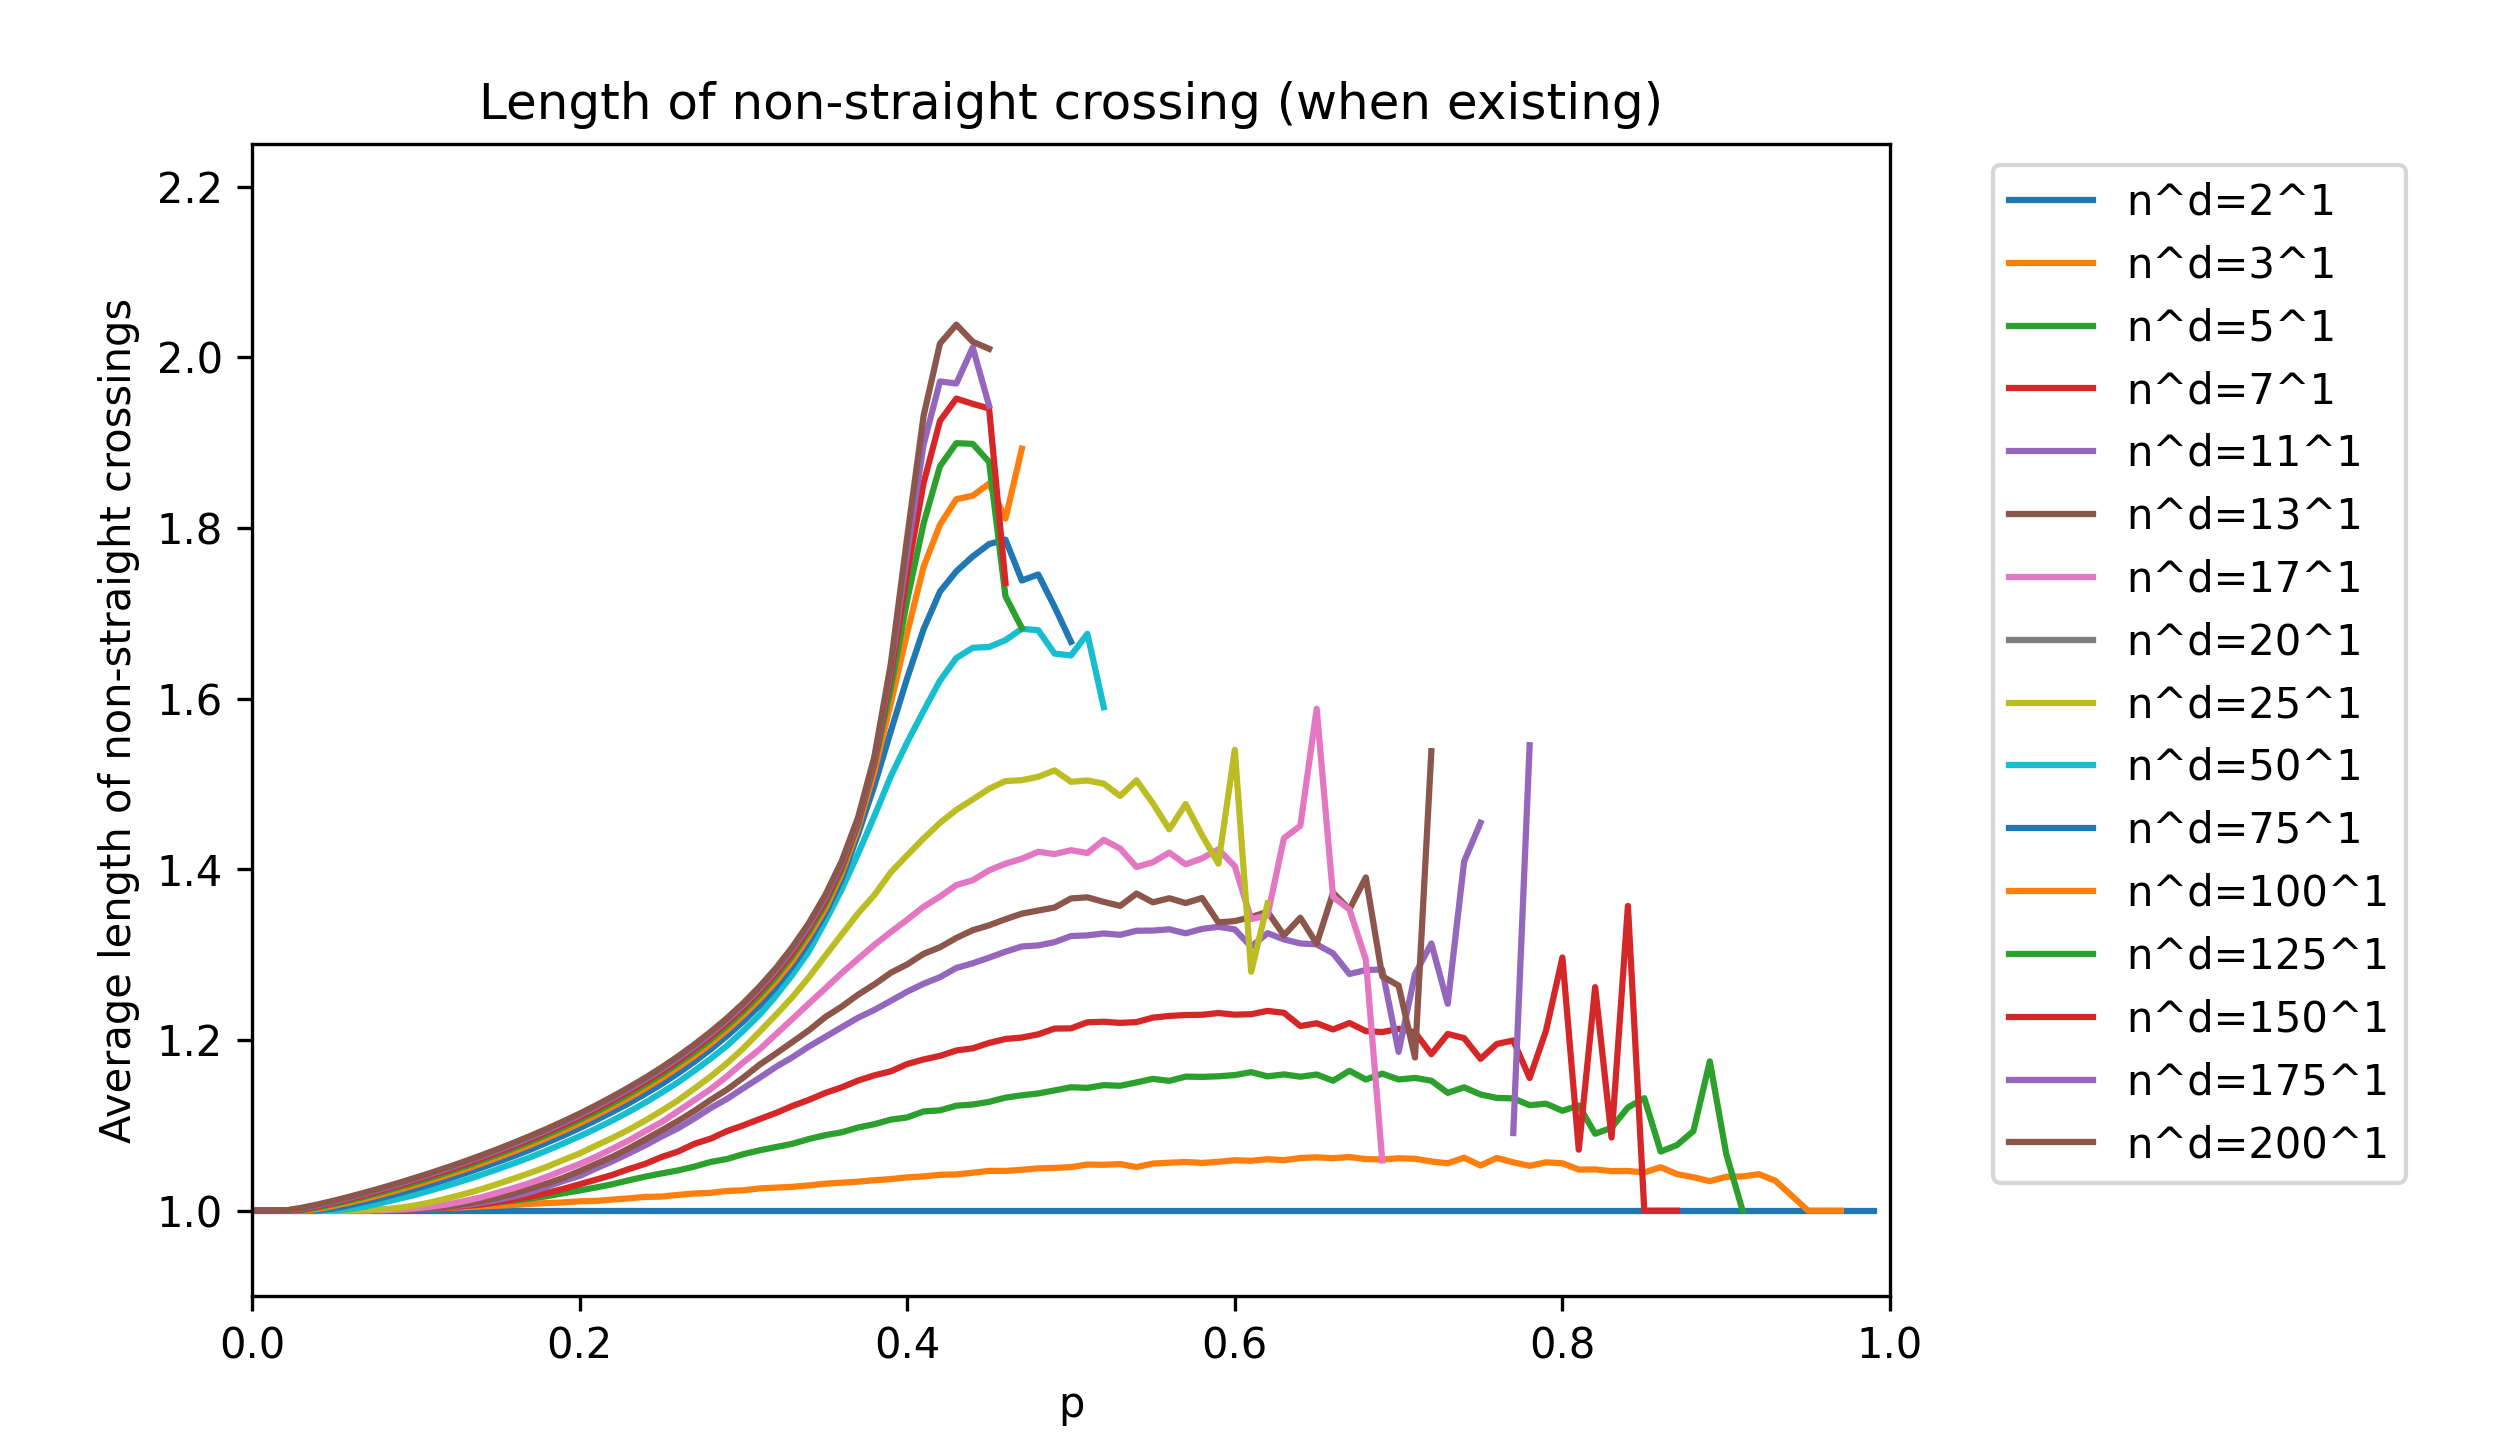
\includegraphics[width=8cm]{complement_crossing_length_2D_ter}
		\centering
		\captionsetup{justification=centering}
		\caption{Classical Percolation}
	\end{subfigure}
	\hspace{0.1 \linewidth}
	\begin{subfigure}{0.44\linewidth}
		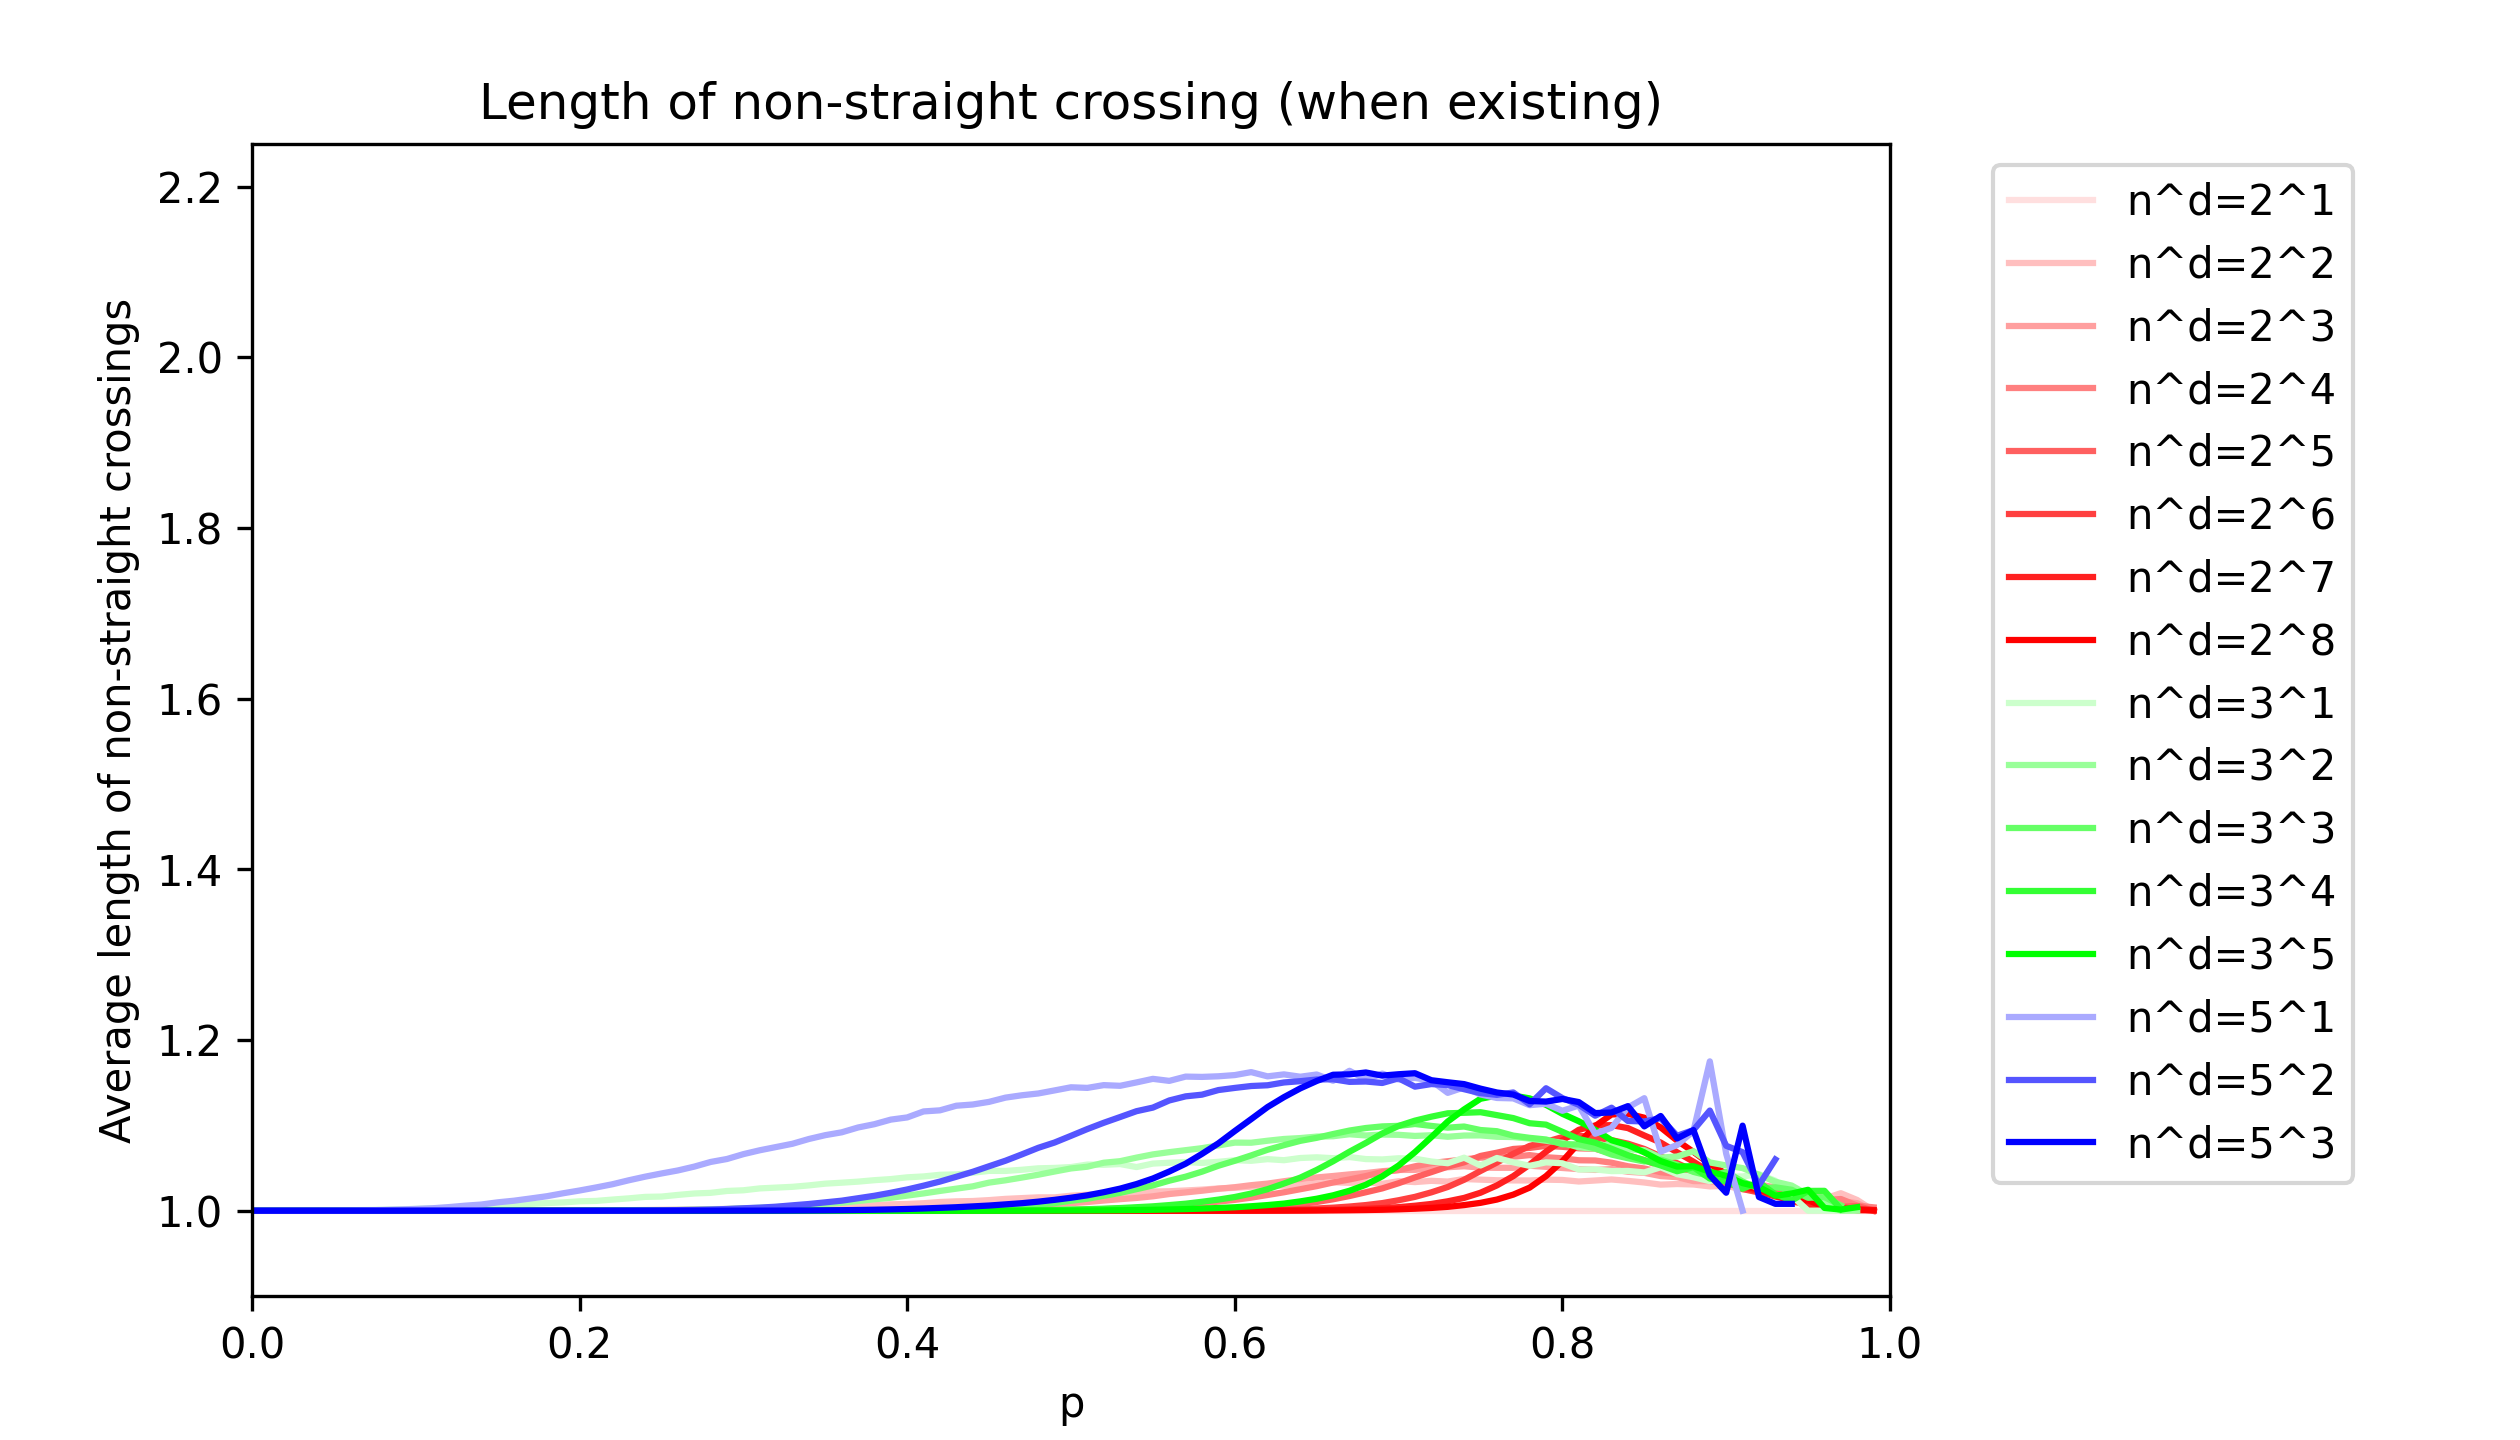
\includegraphics[width=8cm]{complement_crossing_length_2D}
		\centering
		\captionsetup{justification=centering}
		\caption{Recursive Percolation}
	\end{subfigure}
	\caption{Crossings average length on percolation complement (non-straight case).}
	\label{fig:crossingComplementLengths}
\end{figure}

\subsection{Link Between Crossings and Complement Crossings}
In the case of $D=2$, vertical (respectively horizontal) crossing on $P$ is incompatible with horizontal (respectively vertical) crossing of $P^C$.

Since we proved that if $p \leq \nicefrac{1}{\sqrt{n}}$, then $P^C$ has a crossing with probability one, we get as a consequence that $P$ has a crossing with probability zero (note that the existence probability of a vertical crossing is the same as the one of an horizontal crossing, by symmetry).

\subsection{Connectivity Properties}
Some properties of percolations are already known by the community.
We will look here at the ones regarding connectivity of the percolation, which are related to crossings.
Most results were stated in two dimensions in the literature.
When possible, we will generalize the results to dimension $D$.

\paragraph{Almost Sure Disconnectedness}
If $p \leq \nicefrac{1}{\sqrt{n^{D-1}}}$, then the largest connected component in a percolation $P \sim \text{Perc}^D(n,p,\infty)$ is a point (almost surely).

The following proof uses techniques from \cite[p.310 b.(2)]{Chayes_1988}
\begin{proof}
	Similarly to last proof (see section \ref{prf:nonStraightComplementCrossigs}), we say that a facet 
	$$f_{j_1,\dots,j_D}^k = \left\lbrace \frac{j_1}{n^k} \right\rbrace \times \left( \prod_{i=2}^{D} \left[ \frac{j_i-1}{n^k},\frac{j_i}{n^k} \right] \right) $$
	is vacant if either of the two adjacent cuboids in the $k^{th}$ filtration is.
	
	Let $Y^k$ be the number of occupied facets for the form $f_{j_1,\dots,j_D}^k$ after $k$ filtrations.
	$Y^k$ is a branching process in which each element has $p^2n^{D-1}$ offsprings.
	Now, if $p^2n^{D-1}	\leq 1$ (i.e. $p \leq \nicefrac{1}{\sqrt{n^{D-1}}}$), then the branching process will die out with probability one.
	Similarly to last proof, if we wait long enough, it is almost sure that there will be a hyper-surface\footnote{Here, hyper-surface and hyperplane are of dimensions $D-1$ in $\R^D$.} in the percolation complement $P^C$ arbitrarily close to the hyperplane $\left\lbrace \frac{j_1}{n^k} \right\rbrace \times \left[ 0,1 \right]^{D-1}$ (see fig. \ref{fig:complementSurface} for examples in two and three dimensions).
	
	Finally, repeating the argument for $j_m \in \left[ 1,n^k\right] $, we get that almost surely, there are hyper-surfaces on the percolation complement arbitrarily close to the hyperplanes $\left\lbrace \frac{j_1}{n^k} \right\rbrace \times \left[ 0,1 \right]^{D-1}$.
	By reflecting the argument, there are some hyper-surfaces arbitrarily close to the hyperplanes $\left[ 0,1 \right]^{m-1} \times \left\lbrace \frac{j_m}{n^k} \right\rbrace \times \left[ 0,1 \right]^{D-m-1}$.
	Therefore, the largest connected component is a point.
\end{proof}

\begin{figure}[!h]
	\vspace{-0.75cm}
	\begin{subfigure}{0.44\linewidth}
		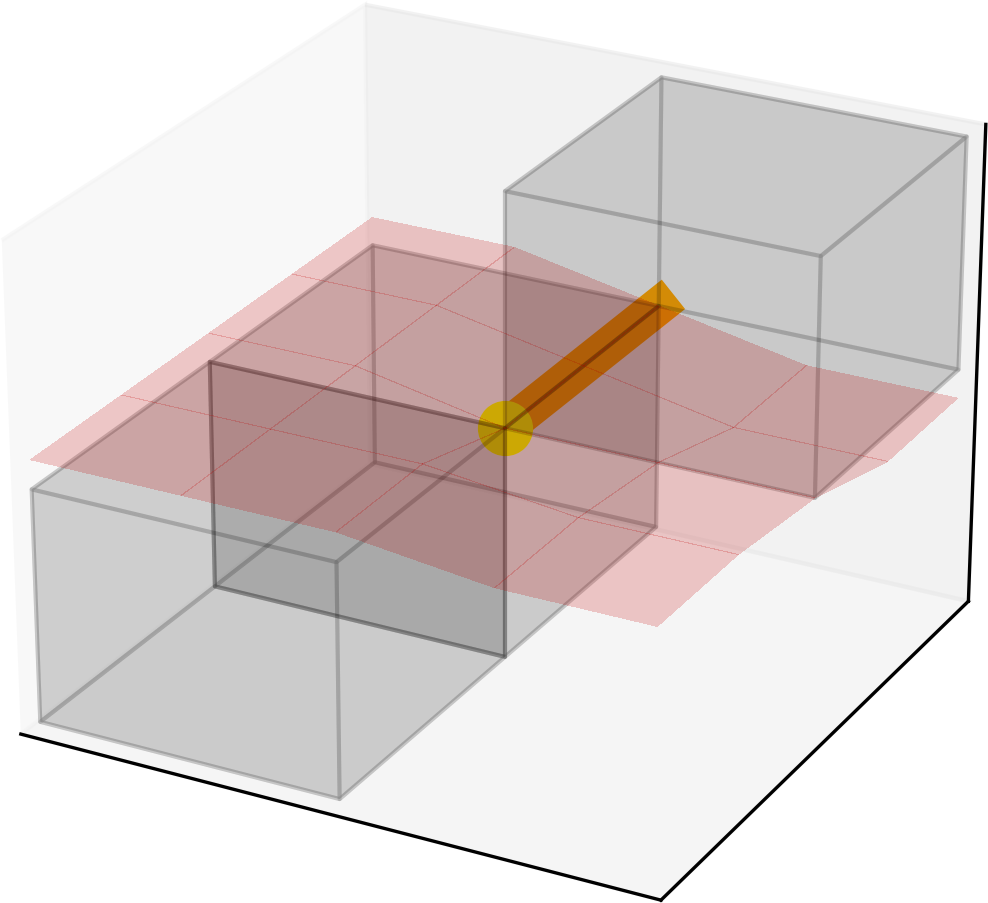
\includegraphics[width=5.25cm]{complement_surface3D}
		\centering
		\captionsetup{justification=centering}
		\caption{$D = 3$\\Hyper-surface is a usual 3D surface.}
		\label{fig:complementSurface3D}
	\end{subfigure}
	\hspace{0.1\linewidth}
	\begin{subfigure}{0.44\linewidth}
		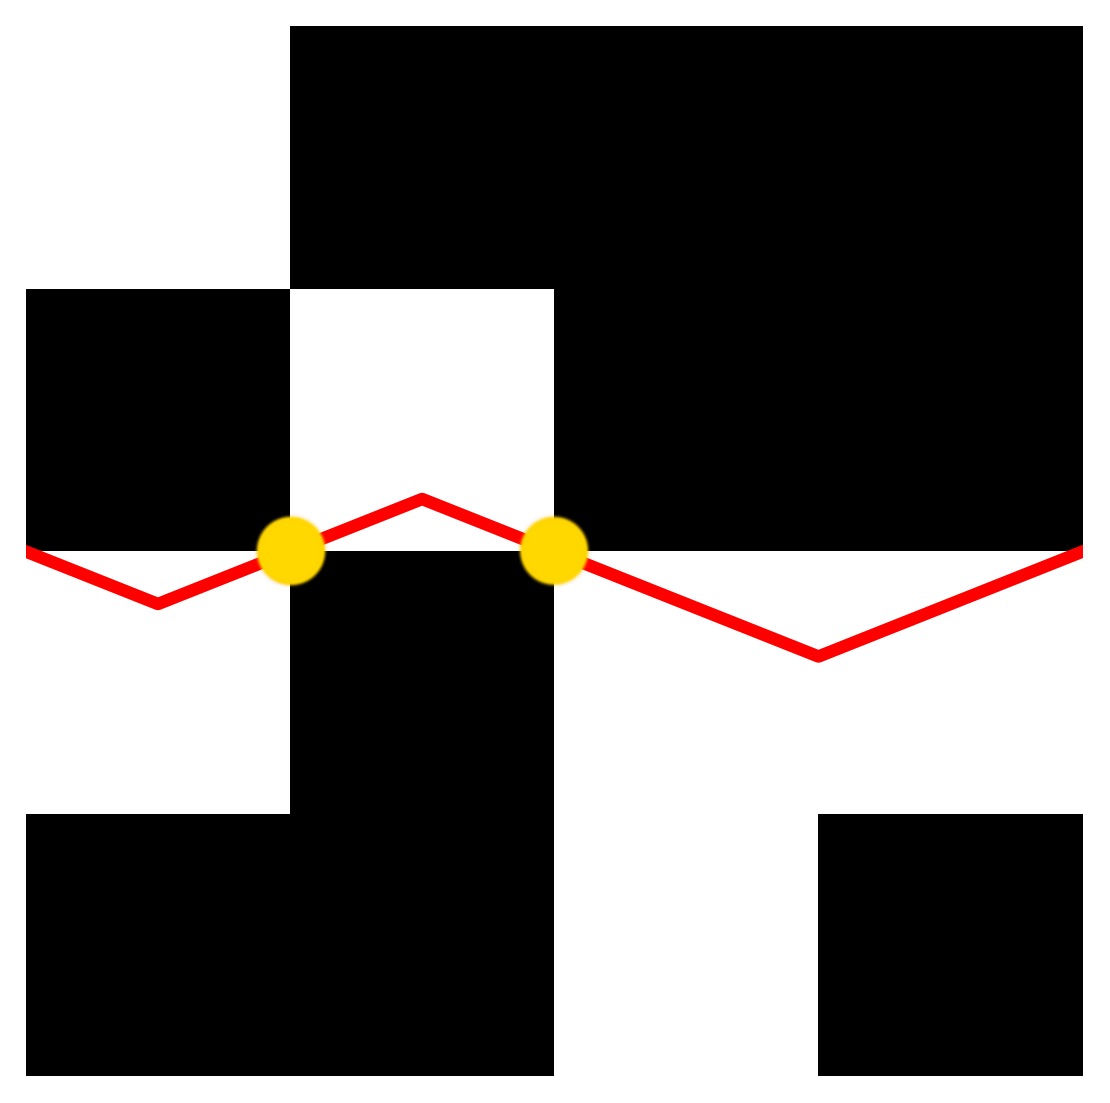
\includegraphics[width=5.25cm]{complement_surface2D}
		\centering
		\captionsetup{justification=centering}
		\caption{$D = 2$\\Hyper-surface is just a line.}
		\label{fig:complementSurface2D}
	\end{subfigure}
	\centering
	\caption{Eventually, the cuboids touching the orange line and yellow point(s) will be removed and the red hyper-surface will remain in full within the percolation complement.}
	\label{fig:complementSurface}
\end{figure}

\paragraph{Minimal Parameter for Crossings to Appear}
It is interesting to study when the percolation starts having crossings.
One defines (notation introduced in \cite{Chayes_1988}) $p_c$ as the minimum value of $p$ such that $P \sim \text{Perc}^D(n,p,\infty)$ has a non zero probability to have a crossing, i.e.
$$p_c = \inf \left\lbrace p \mid \mathbb{P}(P \text{ has a crossing})>0 \right\rbrace .$$

It is reasonable to conjecture that $p_c<1$ for all $n,D \geq 2$. In fact, this was proved in the case $D=2$ in \cite{Chayes_1988}.

Narrowing down to $D=2$:
Chayes et al. proved in \cite{Chayes_1988} that almost surely, if $p<p_c$, the largest connected component of $P$ is a point.
For $p \geq p_c$, the largest connected component is almost surely not a point.
Moreover, we pave $\R^2$ with a percolation $P \sim \text{Perc}^D(n,p,\infty)$ attached at each point of $\Z^2$ (and calling this $P'$).
Then, with probability one, $P'$ has a unique unbounded connected component.
This explains the "jump" behaviour observed in section \ref{blob}.
